% NEED TO BE COMPILED WITH XeLaTeX because I wanna to flex and use emoji

% Options for packages loaded elsewhere
\PassOptionsToPackage{unicode}{hyperref}
\PassOptionsToPackage{hyphens}{url}
%
\documentclass[
]{article}
\usepackage[a4paper, total={6.5in, 10in}]{geometry}
\usepackage{amsmath,amssymb}
\usepackage{iftex}
\ifPDFTeX
  \usepackage[T1]{fontenc}
  \usepackage[utf8]{inputenc}
  \usepackage{textcomp} % provide euro and other symbols
\else % if luatex or xetex
  \usepackage{unicode-math} % this also loads fontspec
  \defaultfontfeatures{Scale=MatchLowercase}
  \defaultfontfeatures[\rmfamily]{Ligatures=TeX,Scale=1}
\fi
\usepackage{lmodern}
\ifPDFTeX\else
  % xetex/luatex font selection
\fi
% Use upquote if available, for straight quotes in verbatim environments
\IfFileExists{upquote.sty}{\usepackage{upquote}}{}
\IfFileExists{microtype.sty}{% use microtype if available
  \usepackage[]{microtype}
  \UseMicrotypeSet[protrusion]{basicmath} % disable protrusion for tt fonts
}{}
\makeatletter
\@ifundefined{KOMAClassName}{% if non-KOMA class
  \IfFileExists{parskip.sty}{%
    \usepackage{parskip}
  }{% else
    \setlength{\parindent}{0pt}
    \setlength{\parskip}{6pt plus 2pt minus 1pt}}
}{% if KOMA class
  \KOMAoptions{parskip=half}}
\makeatother
\usepackage{xcolor}
\usepackage{color}
\usepackage{fancyvrb}
\newcommand{\VerbBar}{|}
\newcommand{\VERB}{\Verb[commandchars=\\\{\}]}
\DefineVerbatimEnvironment{Highlighting}{Verbatim}{commandchars=\\\{\}}
% Add ',fontsize=\small' for more characters per line
\newenvironment{Shaded}{}{}
\newcommand{\AlertTok}[1]{\textcolor[rgb]{1.00,0.00,0.00}{\textbf{#1}}}
\newcommand{\AnnotationTok}[1]{\textcolor[rgb]{0.38,0.63,0.69}{\textbf{\textit{#1}}}}
\newcommand{\AttributeTok}[1]{\textcolor[rgb]{0.49,0.56,0.16}{#1}}
\newcommand{\BaseNTok}[1]{\textcolor[rgb]{0.25,0.63,0.44}{#1}}
\newcommand{\BuiltInTok}[1]{\textcolor[rgb]{0.00,0.50,0.00}{#1}}
\newcommand{\CharTok}[1]{\textcolor[rgb]{0.25,0.44,0.63}{#1}}
\newcommand{\CommentTok}[1]{\textcolor[rgb]{0.38,0.63,0.69}{\textit{#1}}}
\newcommand{\CommentVarTok}[1]{\textcolor[rgb]{0.38,0.63,0.69}{\textbf{\textit{#1}}}}
\newcommand{\ConstantTok}[1]{\textcolor[rgb]{0.53,0.00,0.00}{#1}}
\newcommand{\ControlFlowTok}[1]{\textcolor[rgb]{0.00,0.44,0.13}{\textbf{#1}}}
\newcommand{\DataTypeTok}[1]{\textcolor[rgb]{0.56,0.13,0.00}{#1}}
\newcommand{\DecValTok}[1]{\textcolor[rgb]{0.25,0.63,0.44}{#1}}
\newcommand{\DocumentationTok}[1]{\textcolor[rgb]{0.73,0.13,0.13}{\textit{#1}}}
\newcommand{\ErrorTok}[1]{\textcolor[rgb]{1.00,0.00,0.00}{\textbf{#1}}}
\newcommand{\ExtensionTok}[1]{#1}
\newcommand{\FloatTok}[1]{\textcolor[rgb]{0.25,0.63,0.44}{#1}}
\newcommand{\FunctionTok}[1]{\textcolor[rgb]{0.02,0.16,0.49}{#1}}
\newcommand{\ImportTok}[1]{\textcolor[rgb]{0.00,0.50,0.00}{\textbf{#1}}}
\newcommand{\InformationTok}[1]{\textcolor[rgb]{0.38,0.63,0.69}{\textbf{\textit{#1}}}}
\newcommand{\KeywordTok}[1]{\textcolor[rgb]{0.00,0.44,0.13}{\textbf{#1}}}
\newcommand{\NormalTok}[1]{#1}
\newcommand{\OperatorTok}[1]{\textcolor[rgb]{0.40,0.40,0.40}{#1}}
\newcommand{\OtherTok}[1]{\textcolor[rgb]{0.00,0.44,0.13}{#1}}
\newcommand{\PreprocessorTok}[1]{\textcolor[rgb]{0.74,0.48,0.00}{#1}}
\newcommand{\RegionMarkerTok}[1]{#1}
\newcommand{\SpecialCharTok}[1]{\textcolor[rgb]{0.25,0.44,0.63}{#1}}
\newcommand{\SpecialStringTok}[1]{\textcolor[rgb]{0.73,0.40,0.53}{#1}}
\newcommand{\StringTok}[1]{\textcolor[rgb]{0.25,0.44,0.63}{#1}}
\newcommand{\VariableTok}[1]{\textcolor[rgb]{0.10,0.09,0.49}{#1}}
\newcommand{\VerbatimStringTok}[1]{\textcolor[rgb]{0.25,0.44,0.63}{#1}}
\newcommand{\WarningTok}[1]{\textcolor[rgb]{0.38,0.63,0.69}{\textbf{\textit{#1}}}}
\usepackage{longtable,booktabs,array}
\usepackage{calc} % for calculating minipage widths
% Correct order of tables after \paragraph or \subparagraph
\usepackage{etoolbox}
\makeatletter
\patchcmd\longtable{\par}{\if@noskipsec\mbox{}\fi\par}{}{}
\makeatother
% Allow footnotes in longtable head/foot
\IfFileExists{footnotehyper.sty}{\usepackage{footnotehyper}}{\usepackage{footnote}}
\makesavenoteenv{longtable}
\usepackage{graphicx}
\makeatletter
\def\maxwidth{\ifdim\Gin@nat@width>\linewidth\linewidth\else\Gin@nat@width\fi}
\def\maxheight{\ifdim\Gin@nat@height>\textheight\textheight\else\Gin@nat@height\fi}
\makeatother
% Scale images if necessary, so that they will not overflow the page
% margins by default, and it is still possible to overwrite the defaults
% using explicit options in \includegraphics[width, height, ...]{}
\setkeys{Gin}{width=\maxwidth,height=\maxheight,keepaspectratio}
% Set default figure placement to htbp
\makeatletter
\def\fps@figure{htbp}
\makeatother
\setlength{\emergencystretch}{3em} % prevent overfull lines
\providecommand{\tightlist}{%
  \setlength{\itemsep}{0pt}\setlength{\parskip}{0pt}}
\setcounter{secnumdepth}{-\maxdimen} % remove section numbering
\ifLuaTeX
  \usepackage{selnolig}  % disable illegal ligatures
\fi
\usepackage{bookmark}
\IfFileExists{xurl.sty}{\usepackage{xurl}}{} % add URL line breaks if available
\urlstyle{same}
\hypersetup{
  hidelinks,
  pdfcreator={Résumé (propulsed by Pandoc)}}

\author{Thomas Debelle}
\date{}

\setmainfont{Arial} % Choose a font that supports the desired Unicode characters

\begin{document}

\tableofcontents

\href{../README.md}{\textless--}

\begin{center}\rule{0.5\linewidth}{0.5pt}\end{center}

\textbf{DISCLAIMER:} toutes les illustrations proviennent du cours
dispensé par E. Riviere et ne sont en aucun cas ma propriété.

La synthèse est incomplète, a des erreurs ou autres choses ? Faites une
Pull Request sur le dépôt
\href{https://github.com/Tfloow/LINFO1252}{Github}.

Si la synthèse vous a aidé, n'hésitez pas à rajouter une étoile au
dépôt, ça fait toujours plaisir 🫶.

\section{Cours 1}\label{cours-1}

\subsection{Fondamentaux}\label{fondamentaux}

On a des composants: - RAM, CPU, IO devices, \ldots{}

Le processeur exécute des \emph{instructions}.

\begin{itemize}
\tightlist
\item
  Lire / écrire en mémoire vers / depuis des registres
\item
  Opérations sur ces registres
\end{itemize}

Il y a 2 grandes familles \emph{X86\_64} et \emph{ARM A64} avec des jeux
d'instructions différents.

\subsubsection{Architecture de von
Neumann}\label{architecture-de-von-neumann}

\begin{figure}
\centering
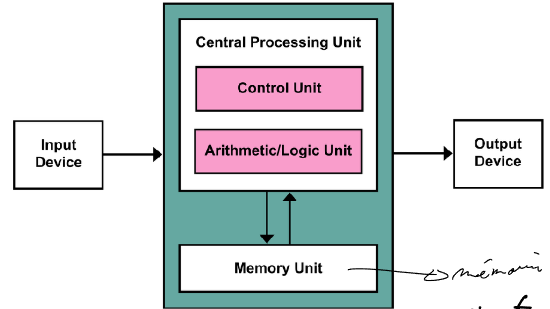
\includegraphics{image-5.png}
\caption{alt}
\end{figure}

\subsection{Représentation des
données}\label{repruxe9sentation-des-donnuxe9es}

On a typiquement:

\begin{longtable}[]{@{}cc@{}}
\toprule\noalign{}
taille & nome \\
\midrule\noalign{}
\endhead
\bottomrule\noalign{}
\endlastfoot
4 bits & nibble \\
8 bits & octet \\
32 bits & mot \\
64 bits & long mot \\
\end{longtable}

\subsection{Fonctionnement d'un système
informatique}\label{fonctionnement-dun-systuxe8me-informatique}

Les opérations d'entrée/sortie se déroulent de manière
\emph{concurrente}. Chacun a un contrôleur qui a une mémoire spécifique.
Le processeur doit transporter les infos de la mémoire classique à la
zone des contrôleurs.

Un processeur n'est pas de base parallélisé. À chaque frappe du clavier,
une \textbf{interruption} est lancée pour intercepté ce stimulis.

\subsubsection{Interruption}\label{interruption}

Le processeur va s'arrêté dans son exécution et va \emph{transférer} le
contrôle du processeur à une routine de traitement.

La routine de traitement va déterminer la source de l'interruption

Il va positionner le compteur de programme à la \emph{première}
exécution du segment de code associé à cette \emph{source}.

À la fin du traitement, on restaure l'état du processeur et on reprend
le processus interrompu en restaurant le compteur de programme

\subsection{Opérations
d'entrée/sorite}\label{opuxe9rations-dentruxe9esorite}

\begin{figure}
\centering
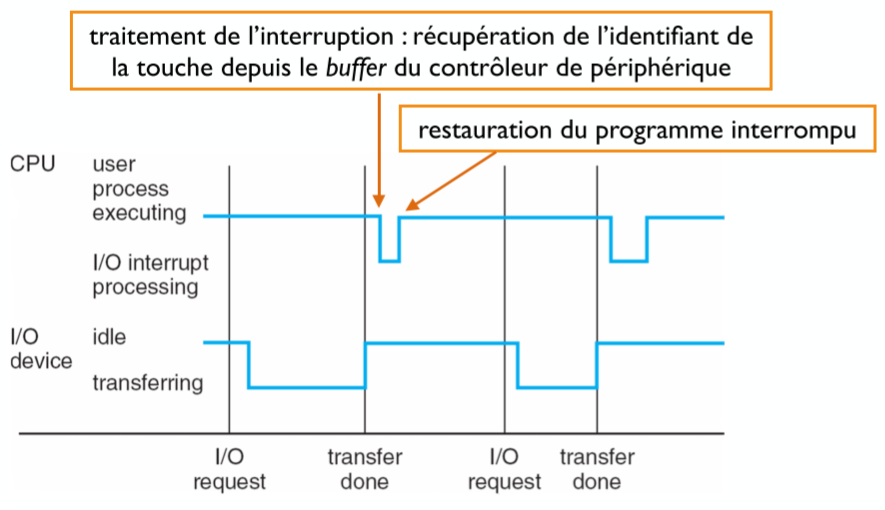
\includegraphics{image.png}
\caption{Alt text}
\end{figure}

\subsection{Accès direct à la
mémoire}\label{accuxe8s-direct-uxe0-la-muxe9moire}

Pour chaque touche de clavier, on doit interrompre pour que le
processeur utilise ces données.

Pour éviter les interruptions qui vont à l'infini, on utilise du
\textbf{DMA} qui est \emph{l'accès direct à la mémoire}. Cela permet un
transfert direct entre le contrôleur de périphérique et la mémoire
principale.

\begin{figure}
\centering
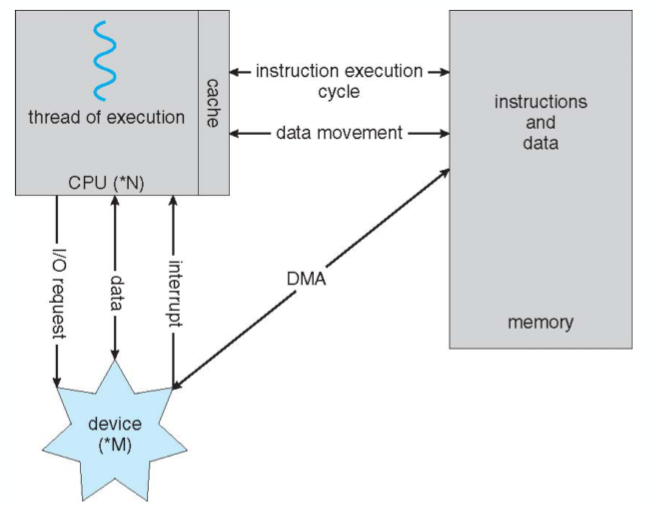
\includegraphics{image-1.png}
\caption{Alt text}
\end{figure}

\subsection{Le rôle du système
d'exploitation}\label{le-ruxf4le-du-systuxe8me-dexploitation}

Le système d'exploitation se met entre l'utilisateur et le matériel. Il
a 3 rôles:

\begin{enumerate}
\def\labelenumi{\arabic{enumi}.}
\tightlist
\item
  Rendre plus simple le développement de programmes
\item
  Utilisation plus efficaces des ressources
\item
  Assurer l'intégrité des données et des programmes entre eux.
\end{enumerate}

\subsection{Virtualisation}\label{virtualisation}

Le système d'exploitation assure cela en \textbf{virtualisant} les
ressources matérielles. On va donc utiliser des API,\ldots{}

\subsubsection{Exemple}\label{exemple}

\begin{itemize}
\tightlist
\item
  Processus
\item
  Le programmeur a l'impression d'avoir tout le processeur
\item
  Processus coexiste et s'entremêle
\item
  Partage du temps dt des ressources
\item
  Virtualisation de la mémoire

  \begin{itemize}
  \tightlist
  \item
    Plusieurs processus en mémoire.
  \item
    On empêche que les autres processus lisent la mémoire des autres
  \item
    Le SE gère la correspondance entre les adresses de la mémoire
    \emph{virtuelle} et les addresses physiques
  \end{itemize}
\end{itemize}

\subsection{Compromis
abstraction/coût}\label{compromis-abstractioncouxfbt}

Cela facilite énormément la vie du programmeur.

\textbf{Mais} on doit à chaque fois recalculer et cela coûte cher en
calcul.

\textbf{Cependant} on a pu réduire ce coût de calcul via l'ajout de
fonctionnalités aux processeurs.

\subsection{Séparation entre mécanisme et
politique}\label{suxe9paration-entre-muxe9canisme-et-politique}

Via la virtualisation par exemple:

\begin{enumerate}
\def\labelenumi{\arabic{enumi}.}
\tightlist
\item
  Mécanisme de partage de temps:

  \begin{itemize}
  \tightlist
  \item
    Changement de contexte: sauvegarde l'état du processeur et restaure
  \end{itemize}
\item
  Politique arbitre entre les processeurs pouvant s'exécuter et les
  processeurs disponibles:

  \begin{itemize}
  \tightlist
  \item
    Politique d'ordonnancement (\emph{scheduling})
  \end{itemize}
\end{enumerate}

On peut donc changer les \emph{politiques d'ordonnancement} différentes
selon les besoins mais avec le même mécanisme.

\subsection{Modes d'exécution}\label{modes-dexuxe9cution}

\begin{itemize}
\tightlist
\item
  \textbf{Utilisateur}: programme utilisant les abstractions fournies
  par le SE.
\item
  \textbf{Protégé}: utilisé par le noyau du SE, toutes les instructions
  sont autorisées
\end{itemize}

L'utilisation de fonctionnalités du SE par un processus utilisateur
nécessite de passer d'un mode à l'autre. (\emph{appel système})

\subsection{Appel système ==
interruption}\label{appel-systuxe8me-interruption}

\begin{figure}
\centering
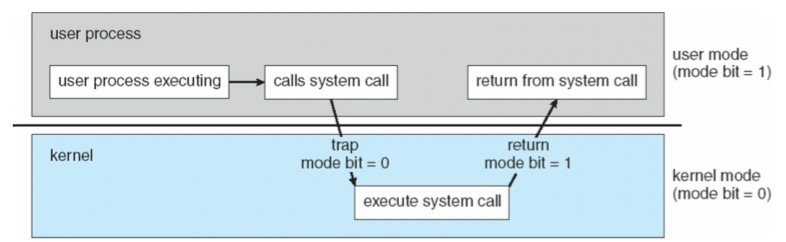
\includegraphics{image-2.png}
\caption{Alt text}
\end{figure}

\subsection{En Résume}\label{en-ruxe9sume}

Système d'exploitation \textasciitilde= traitement des interruptions

\begin{itemize}
\tightlist
\item
  Interruptions matérielles (IO)
\item
  Interruptions du processeur (instructions illégales user)
\item
  Interruptions logicielles (appels systèmes)
\end{itemize}

\subsection{UNIX}\label{unix}

Est une famille de système d'exploitation.

Ici, on verra surtout GNU/Linux. - Linux: kernel - GNU: collection
d'utilitaires et de librairies associés.

\begin{figure}
\centering
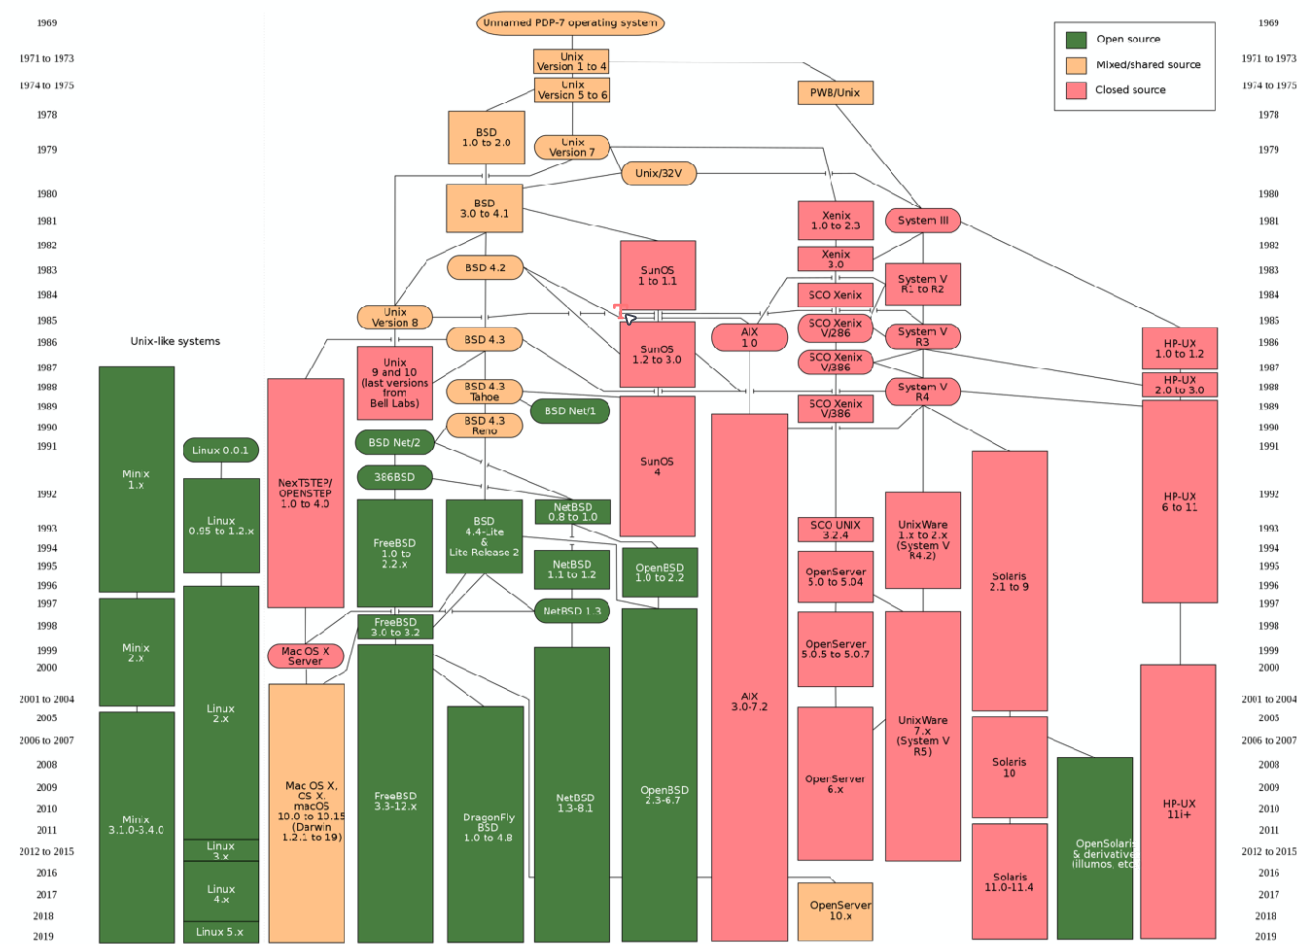
\includegraphics{image-3.png}
\caption{Alt text}
\end{figure}

Il y a la philosophie \emph{KISS}: - \emph{Keep It Simple, Stupid} -
Programme simple, petit, parfaitement adapté à une tâche ou fonction
unique - Facilité de composition de commandes

\begin{longtable}[]{@{}
  >{\centering\arraybackslash}p{(\columnwidth - 2\tabcolsep) * \real{0.1134}}
  >{\centering\arraybackslash}p{(\columnwidth - 2\tabcolsep) * \real{0.8866}}@{}}
\toprule\noalign{}
\begin{minipage}[b]{\linewidth}\centering
Utilitaire
\end{minipage} & \begin{minipage}[b]{\linewidth}\centering
Fonction
\end{minipage} \\
\midrule\noalign{}
\endhead
\bottomrule\noalign{}
\endlastfoot
cat & lire/afficher le contenu d'un fichier. ex :
\texttt{cat\ fichier.txt} \\
echo & afficher une chaîne de caractère \\
head / tail & affiche le début ou la fin d'un fichier \\
wc & compte le nombre de caractères \\
wc & trie un fichier. ex:\texttt{sort\ -n\ -r\ scores.txt} \\
uniq & extrait les lignes uniques ou dupliquées d'un fichier trié. ex:
\texttt{uniq\ -d\ students.dat} \\
\end{longtable}

\subsection{La documentation}\label{la-documentation}

Chaque utilitaire possède une manpage.

\texttt{man\ nom\_utilitaire}

On a des sections de manuelles qui différencies et trie les utilitaires
(librairie standard, appel système, \ldots)

\begin{enumerate}
\def\labelenumi{\arabic{enumi}.}
\tightlist
\item
  Utilitaires disponibles pour tous les utilisateurs
\item
  Appels systèmes en C
\item
  Fonctions de la librairie
\item
  Fichiers spéciaux
\item
  Formats de fichiers et conventions pour certains types de fichiers
\item
  Jeux
\item
  Utilitaires de manipulation de fichier textes
\item
  Commandes et procédure de gestion du système
\end{enumerate}

Donc parfois on doit préciser \texttt{man\ 1\ printf}.

\subsection{Flux standards}\label{flux-standards}

\begin{figure}
\centering
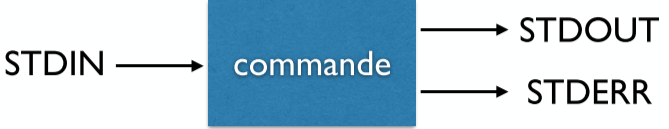
\includegraphics{image-4.png}
\caption{Alt text}
\end{figure}

On a 1 entrées, 1 sorties par défaut dans le shell (STDOUT) et une
sortie d'erreur (STDERR)

\begin{longtable}[]{@{}
  >{\centering\arraybackslash}p{(\columnwidth - 2\tabcolsep) * \real{0.1139}}
  >{\centering\arraybackslash}p{(\columnwidth - 2\tabcolsep) * \real{0.8861}}@{}}
\toprule\noalign{}
\begin{minipage}[b]{\linewidth}\centering
commande
\end{minipage} & \begin{minipage}[b]{\linewidth}\centering
action
\end{minipage} \\
\midrule\noalign{}
\endhead
\bottomrule\noalign{}
\endlastfoot
\texttt{\textless{}\ file} & redirige le contenu de \texttt{file} vers
STDIN \\
\texttt{\textgreater{}\ file} & redirige STDOUT vers \texttt{file} \\
\texttt{\textgreater{}\textgreater{}\ file} & redirige STDOUT vers
\texttt{file} et l'ajoute au bout d'un fichier si existe \\
\texttt{2\textless{}\&1} & redirige STDERR vers STDOUT \\
\end{longtable}

On a aussi des Pipes qui redirige le résultat de commande de STDOUT vers
le STDIN d'une autre commande.

\begin{Shaded}
\begin{Highlighting}[]
\ExtensionTok{cmd1} \KeywordTok{|} \ExtensionTok{cmd2}
\end{Highlighting}
\end{Shaded}

\subsection{Script}\label{script}

En entête de script \emph{interprété} il faut ajouter l'interpréteur
(python, bash):

\begin{Shaded}
\begin{Highlighting}[]
\CommentTok{\#!/bin/bash}
\BuiltInTok{echo} \StringTok{"Hello, world"}
\end{Highlighting}
\end{Shaded}

\subsubsection{Arguments en ligne de
commande}\label{arguments-en-ligne-de-commande}

\begin{Shaded}
\begin{Highlighting}[]
\CommentTok{\#!/bin/bash }
\CommentTok{\# $\# nombre d\textquotesingle{}arguments }
\CommentTok{\# $1 $2 $3 ... arguments }
\BuiltInTok{echo} \StringTok{"Vous avez passé"} \VariableTok{$\#} \StringTok{"arguments"} 
\BuiltInTok{echo} \StringTok{"Le premier argument est :"} \VariableTok{$1}
\BuiltInTok{echo} \StringTok{"Liste des arguments :"} \VariableTok{$@}
\end{Highlighting}
\end{Shaded}

\subsubsection{Retour}\label{retour}

On peut retourner le résultat de la dernière commande via \texttt{\$?}.
Si 0 c'est bon.

On peut envoyer des données dans \texttt{/dev/null} et c'est un trou
noir.

On peut lire du contenu aléatoire dans \texttt{/dev/random}.

\subsubsection{\texorpdfstring{Boucles
\texttt{for}}{Boucles for}}\label{boucles-for}

\begin{Shaded}
\begin{Highlighting}[]
\CommentTok{\#!/bin/bash }
\CommentTok{\# exemple\_for.sh }
\VariableTok{students}\OperatorTok{=}\StringTok{"Julie Maxime Hakim"} 
\ControlFlowTok{for}\NormalTok{ s }\KeywordTok{in} \VariableTok{$students}\KeywordTok{;} \ControlFlowTok{do} 
  \VariableTok{l}\OperatorTok{=}\KeywordTok{\textasciigrave{}}\FunctionTok{wc} \AttributeTok{{-}l}\NormalTok{ TP1{-}}\VariableTok{$s}\NormalTok{.txt }\KeywordTok{|} \FunctionTok{cut} \AttributeTok{{-}d}\StringTok{\textquotesingle{} \textquotesingle{}} \AttributeTok{{-}f1}\KeywordTok{\textasciigrave{}} 
  \BuiltInTok{echo} \StringTok{"Bonjour }\VariableTok{$s}\StringTok{, ton compte rendu de TP comporte }\VariableTok{$l}\StringTok{ lignes."}
\ControlFlowTok{done}
\end{Highlighting}
\end{Shaded}

\begin{itemize}
\tightlist
\item
  s prend successivement les valeurs présentes dans la liste d'entrée
  \texttt{\$students}
\end{itemize}

\begin{center}\rule{0.5\linewidth}{0.5pt}\end{center}

\href{../README.md}{\textless--}

\href{../README.md}{\textless--}

\begin{center}\rule{0.5\linewidth}{0.5pt}\end{center}

\section{Rappels \& compléments de C}\label{rappels-compluxe9ments-de-c}

\begin{itemize}
\tightlist
\item
  \hyperref[rappels--compluxe9ments-de-c]{Rappels \& compléments de C}

  \begin{itemize}
  \tightlist
  \item
    \hyperref[les-bases]{Les bases}

    \begin{itemize}
    \tightlist
    \item
      \hyperref[hello-world]{Hello world}
    \item
      \hyperref[pruxe9processeur]{Préprocesseur}
    \item
      \hyperref[types-de-variables]{Types de variables}
    \item
      \hyperref[tableaux]{Tableaux}
    \item
      \hyperref[caractuxe8res-ascii]{Caractères ASCII}
    \item
      \hyperref[les-pointeurs]{Les pointeurs}
    \item
      \hyperref[structures]{Structures}
    \item
      \hyperref[pointeur-vers-une-fonction]{Pointeur vers une fonction}
    \item
      \hyperref[expressions-de-manipulation-de-bits]{Expressions de
      manipulation de bits}
    \item
      \hyperref[constante]{Constante}
    \end{itemize}
  \end{itemize}
\end{itemize}

\subsection{Les bases}\label{les-bases}

\subsubsection{Hello world}\label{hello-world}

On se souvient que pour faire un programme en C il faut des choses
cruciales: 1. Directives préprocesseur
\texttt{\#include\ \textless{}stdio.h\textgreater{}} 2. Avoir une
fonction \texttt{main} qui est le point d'entrée de l'exécution 1.
Fournir les arguments \texttt{argc} et \texttt{argv{[}{]}} pour prendre
les arguments en ligne de commande. 3. Retourner un succès avec
\texttt{EXIT\_SUCCESS} 4. Compiler le programme avec \texttt{gcc} comme
cela \texttt{gcc\ -o\ output\ input.c}

\begin{Shaded}
\begin{Highlighting}[]
\PreprocessorTok{\#include }\ImportTok{\textless{}stdio.h\textgreater{}}
\PreprocessorTok{\#include }\ImportTok{\textless{}stdlib.h\textgreater{}}

\DataTypeTok{int}\NormalTok{ main}\OperatorTok{(}\DataTypeTok{int}\NormalTok{ argc}\OperatorTok{,} \DataTypeTok{char}\OperatorTok{*}\NormalTok{ argv}\OperatorTok{[])\{}
\NormalTok{    printf}\OperatorTok{(}\StringTok{"Hello world !}\SpecialCharTok{\textbackslash{}n}\StringTok{"}\OperatorTok{);}

    \ControlFlowTok{return}\NormalTok{ EXIT\_SUCCESS}\OperatorTok{;}
\OperatorTok{\}}
\end{Highlighting}
\end{Shaded}

\subsubsection{Préprocesseur}\label{pruxe9processeur}

Notre code C est transformé par ce préprocesseur avant d'être compilé en
langage machine.

C'est donc une traduction texte vers texte.

Pour obtenir le résultat du préprocesseur on fait \texttt{gcc\ -E}.

\paragraph{Include et header}\label{include-et-header}

Cela permet d'importer des fonctions, constantes d'un librairie.

\begin{itemize}
\tightlist
\item
  \textbf{Header}: contient les informations sur comment appeler une
  fonction et le squelette du code.
\item
  \textbf{Code source}: la mise en oeuvre des fonctions.
\end{itemize}

On fait \texttt{\#include\ "monheader.h"} pour inclure du dossier
courant et \texttt{\#include\ \textless{}header.h\textgreater{}} pour un
header standard. On peut avoir des infos sur un header via
\texttt{man\ 3\ stdio.h}.

\subsubsection{Types de variables}\label{types-de-variables}

Voir les slides car très basique

Il faut faire attention en C avec les notations des \texttt{int}: -
Notation classique: \texttt{i\ =\ 123} - Hexadécimal:
\texttt{i\ =\ 0x7b} - Octal: \texttt{i\ =\ 0173} - Binaire:
\texttt{i\ =\ 0b1111011}

La différence entre octal et classique est ce 0 au début.

On se souvient aussi des entiers \emph{unsigned} qui sont des entiers
qui ne peuvent être négatifs et donc pour le même nombre de bit peuvent
avoir un nombre plus élevé que leurs homologues \emph{signed}.

\subsubsection{Tableaux}\label{tableaux}

On se souvient qu'en C, la taille d'un array doit être connu à l'avance
! (sinon on doit utiliser malloc sur le heap)

\subsubsection{Caractères ASCII}\label{caractuxe8res-ascii}

\begin{figure}
\centering
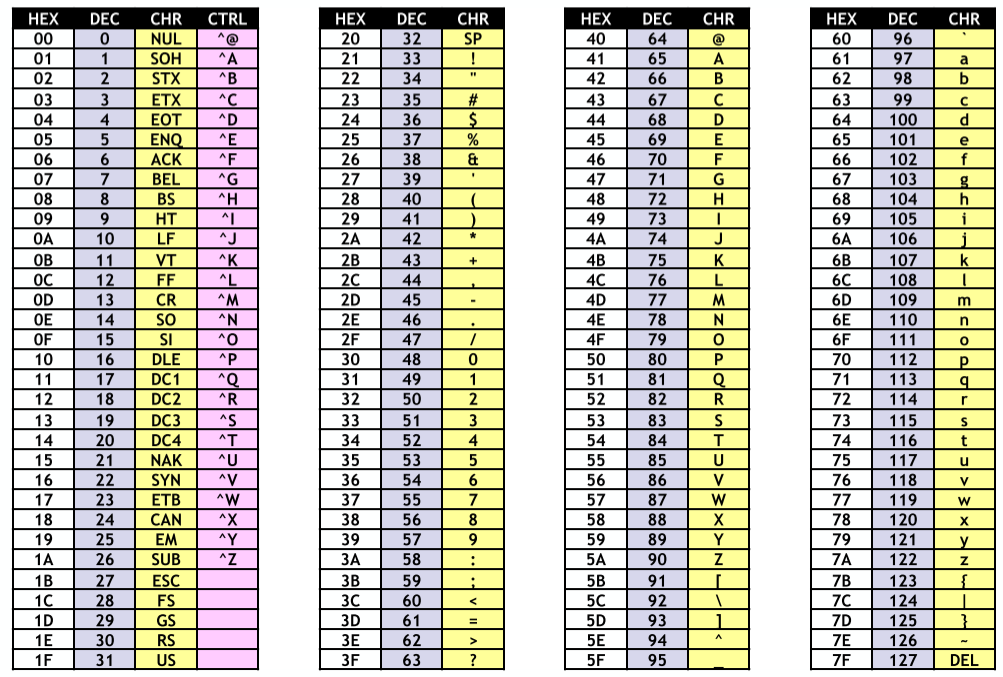
\includegraphics{image-6.png}
\caption{Alt text}
\end{figure}

\subsubsection{Les pointeurs}\label{les-pointeurs}

La mémoire est une sorte de ruban avec des cases (\emph{octets}) avec
des adresses consécutives. Les adresses sont des \textbf{entiers non
signés} de \textbf{32/64} bits selon le processeur ou jeu d'instruction.

Pour définir une variable d'un pointeur on fait:

\begin{Shaded}
\begin{Highlighting}[]
\DataTypeTok{int}\OperatorTok{*}\NormalTok{ ptr\_i}\OperatorTok{;} \CommentTok{// Défini un pointeur d\textquotesingle{}un int}
\OperatorTok{\&}\NormalTok{ptr\_i}\OperatorTok{;} \CommentTok{// Permet d\textquotesingle{}avoir l\textquotesingle{}adresse où est stocké ce pointeur}
\OperatorTok{*}\NormalTok{ptr\_i}\OperatorTok{;} \CommentTok{// Pour avoir la valeur pointée par le pointeur}
\end{Highlighting}
\end{Shaded}

On n'oublie pas qu'on peut faire des \textbf{opérations arithmétiques}
sur les pointeurs. (ex: aller à la case suivante, \ldots)

\begin{Shaded}
\begin{Highlighting}[]
\DataTypeTok{int}\NormalTok{ main}\OperatorTok{(}\DataTypeTok{int}\NormalTok{ argc}\OperatorTok{,} \DataTypeTok{char} \OperatorTok{**}\NormalTok{argv}\OperatorTok{)} \OperatorTok{\{} 
    
    \DataTypeTok{char} \OperatorTok{**}\NormalTok{p}\OperatorTok{;}\NormalTok{ p}\OperatorTok{=}\NormalTok{argv}\OperatorTok{;} 
\NormalTok{    printf}\OperatorTok{(}\StringTok{"Arguments :"}\OperatorTok{);} 
    \ControlFlowTok{while}\OperatorTok{(*}\NormalTok{p}\OperatorTok{!=}\NormalTok{NULL}\OperatorTok{)} \OperatorTok{\{} 
\NormalTok{        printf}\OperatorTok{(}\StringTok{" }\SpecialCharTok{\%s}\StringTok{"}\OperatorTok{,*}\NormalTok{p}\OperatorTok{);} 
\NormalTok{        p}\OperatorTok{++;}
    \OperatorTok{\}}
\NormalTok{    printf}\OperatorTok{(}\StringTok{"}\SpecialCharTok{\textbackslash{}n}\StringTok{"}\OperatorTok{);}
    \ControlFlowTok{return}\OperatorTok{(}\NormalTok{EXIT\_SUCCESS}\OperatorTok{);}
\OperatorTok{\}}
\end{Highlighting}
\end{Shaded}

Ici, on voit que à un moment donné, le pointeur sera \texttt{NULL} car
il n'y a plus de zone mémoire.

\subsubsection{Structures}\label{structures}

On n'a pas la notion d'objet en C mais on peut déclarer des types de
données personnalisées sous forme de structure.

\begin{Shaded}
\begin{Highlighting}[]
\KeywordTok{struct}\NormalTok{ coord}\OperatorTok{\{}
    \DataTypeTok{int}\NormalTok{ x}\OperatorTok{;}
    \DataTypeTok{int}\NormalTok{ y}\OperatorTok{;}
    \DataTypeTok{int}\NormalTok{ z}\OperatorTok{;}
\OperatorTok{\}}

\KeywordTok{struct}\NormalTok{ coord point }\OperatorTok{=} \OperatorTok{\{}\DecValTok{1}\OperatorTok{,} \DecValTok{2}\OperatorTok{,} \DecValTok{3}\OperatorTok{\};}
\NormalTok{point}\OperatorTok{.}\NormalTok{x}\OperatorTok{;}\NormalTok{ point}\OperatorTok{.}\NormalTok{y}\OperatorTok{;}\NormalTok{ point}\OperatorTok{.}\NormalTok{z}\OperatorTok{;}
\end{Highlighting}
\end{Shaded}

\paragraph{Alias}\label{alias}

Pour simplifier l'écriture de structure, on peut utiliser des
\textbf{alias}. On peut même renommer des types de données déjà existant
(ex: int, \ldots):

\begin{Shaded}
\begin{Highlighting}[]
\CommentTok{// structure pour stocker une fraction }
\KeywordTok{typedef} \KeywordTok{struct}\NormalTok{ fraction }\OperatorTok{\{} 
    \DataTypeTok{double}\NormalTok{ numerator}\OperatorTok{;} 
    \DataTypeTok{double}\NormalTok{ denominator}\OperatorTok{;} 
\OperatorTok{\}}\NormalTok{ Fraction }\OperatorTok{;}

\KeywordTok{typedef} \DataTypeTok{int}\NormalTok{ Entier}\OperatorTok{;}

\DataTypeTok{int}\NormalTok{ main}\OperatorTok{(}\DataTypeTok{int}\NormalTok{ argc}\OperatorTok{,} \DataTypeTok{char} \OperatorTok{*}\NormalTok{argv}\OperatorTok{[])} \OperatorTok{\{}
\NormalTok{    Fraction demi }\OperatorTok{=} \OperatorTok{\{}\DecValTok{1}\OperatorTok{,} \DecValTok{2}\OperatorTok{\};} 
\NormalTok{    Entier i }\OperatorTok{=} \DecValTok{2}\OperatorTok{;} 
    \CommentTok{// ... }
    \ControlFlowTok{return}\NormalTok{ EXIT\_SUCCESS}\OperatorTok{;}
\OperatorTok{\}}
\end{Highlighting}
\end{Shaded}

\paragraph{Tips}\label{tips}

Il existe un sucre syntaxique vraiment sympa:

\begin{Shaded}
\begin{Highlighting}[]
\OperatorTok{(*}\NormalTok{f}\OperatorTok{).}\NormalTok{value}\OperatorTok{;}
\NormalTok{f}\OperatorTok{{-}\textgreater{}}\NormalTok{value}\OperatorTok{;}
\end{Highlighting}
\end{Shaded}

Cela fait la même chose mais est plus simple (surtout avec les
parenthèses).

\subsubsection{Pointeur vers une
fonction}\label{pointeur-vers-une-fonction}

On peut stocker une fonction via son pointeur comme cela:

\begin{Shaded}
\begin{Highlighting}[]
\NormalTok{type\_retour }\OperatorTok{(*}\NormalTok{ptr\_vers\_func}\OperatorTok{)([}\NormalTok{type\_arg}\OperatorTok{]+);}
\DataTypeTok{void} \OperatorTok{(*}\NormalTok{f1}\OperatorTok{)(}\DataTypeTok{int}\OperatorTok{,} \DataTypeTok{int}\OperatorTok{,} \DataTypeTok{char}\OperatorTok{*);}
\DataTypeTok{int} \OperatorTok{(*}\NormalTok{f2}\OperatorTok{)(}\DataTypeTok{int}\OperatorTok{);}
\NormalTok{f2 }\OperatorTok{=} \OperatorTok{\&}\NormalTok{ma\_function}\OperatorTok{;}
\end{Highlighting}
\end{Shaded}

Ensuite pour faire un appel, on doit déréférencer le pointeur.

\subsubsection{Expressions de manipulation de
bits}\label{expressions-de-manipulation-de-bits}

\begin{longtable}[]{@{}cc@{}}
\toprule\noalign{}
Opération & Explication \\
\midrule\noalign{}
\endhead
\bottomrule\noalign{}
\endlastfoot
\texttt{\textasciitilde{}} & Inversion des bits \\
\texttt{\&} & Le ET \\
\texttt{\textbackslash{}\textbar{}} & le OU \\
\texttt{\^{}} & le XOR (seulement si 1 bit est 1) \\
\texttt{\textgreater{}\textgreater{}} & Shift les bits de x places vers
la droite \\
\end{longtable}

\subsubsection{Constante}\label{constante}

Pour définir une constante: - \textbf{Avant C99}:
\texttt{\#define\ M\_PI} puis mettre \texttt{3.14159;} - \textbf{Après
C99}: On utilise le mot-clé \texttt{const}.

Une variable globale est définie pour tous les modules d'un programme.

Une variable \texttt{static}, on peut y accéder en dehors d'un bloc de
fonction car on ne doit pas l'instancier.

\begin{center}\rule{0.5\linewidth}{0.5pt}\end{center}

\href{../README.md}{\textless--}

\href{../README.md}{\textless--}

\begin{center}\rule{0.5\linewidth}{0.5pt}\end{center}

\section{Cours 3}\label{cours-3}

\subsection{Déclaration de la
mémoire}\label{duxe9claration-de-la-muxe9moire}

Exécuter un programme sous Unix c'est créé un \emph{nouveau processus} +
\emph{nouvel espace mémoire spécifique} au processus.

\begin{figure}
\centering
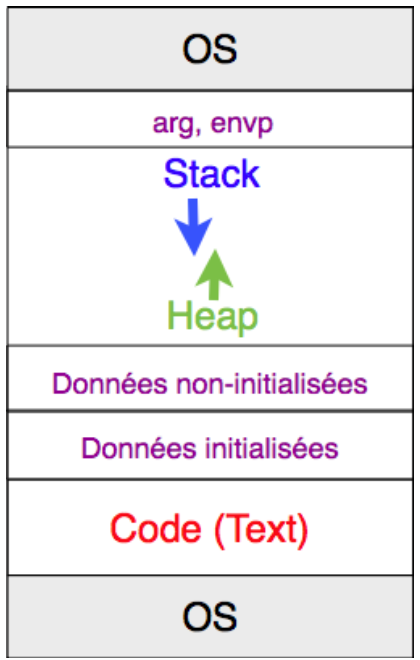
\includegraphics{image-47.png}
\caption{Organisation de la mémoire}
\end{figure}

On a donc 6 segments distincts.

\begin{longtable}[]{@{}
  >{\centering\arraybackslash}p{(\columnwidth - 2\tabcolsep) * \real{0.1590}}
  >{\centering\arraybackslash}p{(\columnwidth - 2\tabcolsep) * \real{0.8410}}@{}}
\toprule\noalign{}
\begin{minipage}[b]{\linewidth}\centering
Zone
\end{minipage} & \begin{minipage}[b]{\linewidth}\centering
Description
\end{minipage} \\
\midrule\noalign{}
\endhead
\bottomrule\noalign{}
\endlastfoot
OS & Réservé à l'OS \\
Segment text & partie la plus basse, en read only. Contient les
instructions à exécuter. Écrire dessus va déclencher un \emph{trap} et
le SE prend le contrôle \\
\emph{Statique}: initialisée & (statique correspond à des données
connues avant l'exécution). Explicitement initialisée ou statique \\
\emph{Statique}: non-initialisée & mise à 0 par le compilateur. \\
Heap & juste après les non-init. Un programme peut y réserver de la
mémoire dessus. On reçoit un pointeur vers le début de la zone.
(\texttt{malloc}) \\
Stack & Démarre vers le haut de l'espace mémoire. Cela stocke les
variables \textbf{locales} et permet l'appel de fonction. (paramètre
d'appel, valeur de retour) et c'est LIFO. \\
Arguments et varaibles d'environnement & Tout d'au-dessus, on a les
données fournies par le SE en lecture seule. Typiquement les données
qu'on passe quand on lance un programme + variable d'environnement
(\texttt{getenv}, \texttt{unsetenv}, \texttt{setenv}, \ldots). \\
\end{longtable}

Il faut savoir que les variables locales non initialisées \textbf{ne
sont pas mises à 0}. Donc attention au garbage data !

\subsection{Gestion de la mémoire
dynamique}\label{gestion-de-la-muxe9moire-dynamique}

L'allocation de mémoire dynamique est une partie de la librairie
standard. On peut parfois faire des appels systèmes pour étendre la zone
mémoire liée au heap.

\begin{figure}
\centering
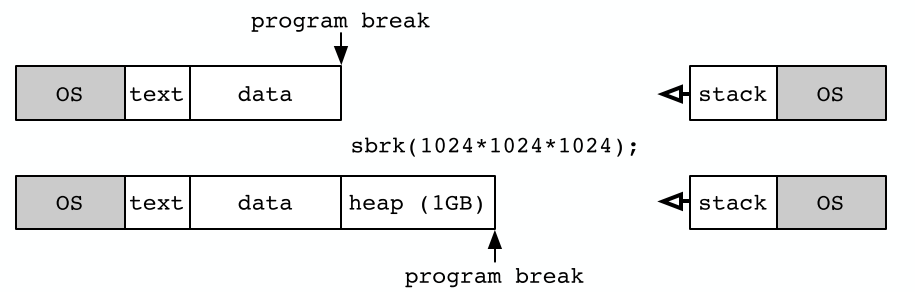
\includegraphics{image-48.png}
\caption{Gestion du heap}
\end{figure}

On voit que \texttt{sbrk} réalise un élargissement de la zone de heap.

\begin{Shaded}
\begin{Highlighting}[]
\PreprocessorTok{\#include }\ImportTok{\textless{}unistd.h\textgreater{}}\PreprocessorTok{ }

\DataTypeTok{int}\NormalTok{ brk}\OperatorTok{(}\DataTypeTok{void} \OperatorTok{*}\NormalTok{addr}\OperatorTok{);}            \CommentTok{// Positionne le programme break a une adresse}
\DataTypeTok{void} \OperatorTok{*}\NormalTok{sbrk}\OperatorTok{(}\DataTypeTok{intptr\_t}\NormalTok{ increment}\OperatorTok{);} \CommentTok{// Décale le programme break et retourne le nouveau program break. (sbrk(0) retourne la valeur actuelle donc)}
\end{Highlighting}
\end{Shaded}

Attention à ne pas trop incrémenter sous peine de cause une erreur.
--\textgreater{} \texttt{ENOMEM} et le processus sera arrêté par le SE.
La limite se trouve via \texttt{ulimit\ -a}.

\subsubsection{Allouer de la mémoire}\label{allouer-de-la-muxe9moire}

On a différentes contraintes: - Conserver l'information sur les blocs
libres et allouées (via méta-données) - méta-données dans le heap -
Trouver le bon endroit pour les mettre

\paragraph{Alignement}\label{alignement}

Les données dans la mémoire sont toutes \textbf{alignées}. Souvent sous
un nombre d'octets entiers --\textgreater{} multiple de 2. Sous linux
c'est 16 octets (128bits).

Donc allouer 17 octets va en réalité nous couter 32 octets.

L'utilité principale (comme vu dans le projet) est que les bits de poids
faibles seront toujours à 0. (effectivement \texttt{0b00000000}
--\textgreater{} \texttt{0b00010000} --\textgreater{}
\texttt{0b00100000} --\textgreater{} \ldots). Ainsi, on peut prendre
avatange de ces 4 bits toujours mis à 0 en les utilisant comme des
méta-données.

\paragraph{Objectifs}\label{objectifs}

\begin{center}\rule{0.5\linewidth}{0.5pt}\end{center}

\href{../README.md}{\textless--}

\section{Cours 4}\label{cours-4}

\subsection{Rappel}\label{rappel}

\subsubsection{Neumann}\label{neumann}

On se souvient de la structure de Neumann où on va stocker en mémoire
\textbf{les instructions et les données}.

Ceci est composé d'un CPU qui a lui même:

\begin{itemize}
\tightlist
\item
  \textbf{Unité arithmétique et logique}: Opérateurs matériel pour les
  opérations \emph{arithmétiques} (\texttt{+,-,...}) et \emph{logiques}
  (\texttt{\&,\textbar{},\^{},...}).
\item
  \textbf{Unité de commande}: Met en oeuvre le cycle
  \emph{fetch/decode/execute} des instructions depuis la mémoire.
\end{itemize}

\subsection{Mémoire}\label{muxe9moire}

On l'organise en octet d'adresses consécutives. \(2^k\) octets donne le
nombre d'adresse mémoire possible sur \(k\) bits. Avec \(k=32\) on a une
taille de mémoire de maximum 4GO contre 16 Exa-octets pour \(k=64\).

\subsubsection{Instructions et
Registres}\label{instructions-et-registres}

On code les instructions en binaires. Les instructions sont de tailles
fixes ou variables.

Un processeur possède un \textbf{nombre limité de zone mémoire} appelés
\textbf{registres}. C'est directement accessible par les instructions et
en tandem avec la mémoire principale.

\subsubsection{Architecture}\label{architecture}

\begin{figure}
\centering
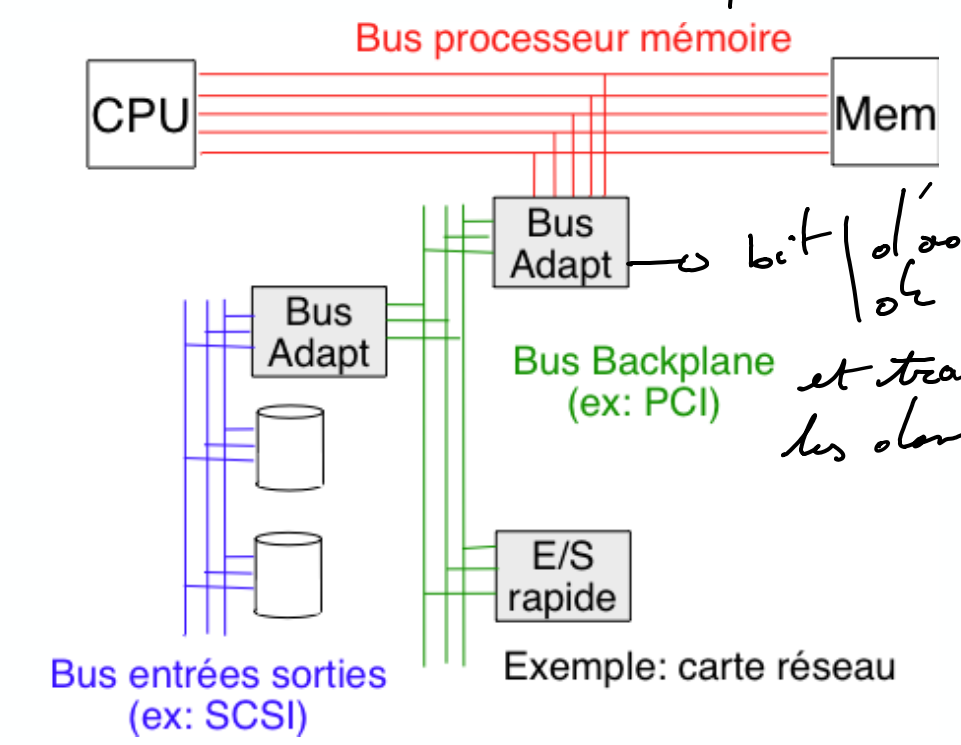
\includegraphics{image-7.png}
\caption{Alt text}
\end{figure}

\subsubsection{Technologies mémoires}\label{technologies-muxe9moires}

On a la \textbf{SRAM} (statique) et la \textbf{DRAM} (dynamique). La
SRAM est plus couteuse mais plus rapide. On va les utiliser en tandem
pour ne pas être ralenti par notre mémoire.

En effet, les cycles de CPU sont devenus extrêment court. Encore plus
court que ceux de la mémoire. C'est-à-dire on perdrait ce gain de
vitesse si on utilisait que de la DRAM car on devrait attendre pour
plusieurs cycles avant d'avoir l'information.

Ces deux technologies sont dites \textbf{volatiles}. Quand plus de jus
c'est mort.

\paragraph{SRAM}\label{sram}

\begin{figure}
\centering
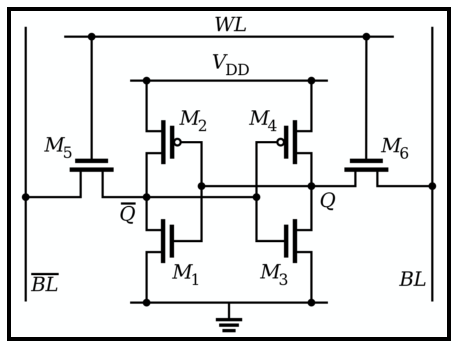
\includegraphics{image-8.png}
\caption{SRAM}
\end{figure}

On a donc de multiples bascules (6 transistor par bit (ou 4 + des
resistances)). On lit la valeur en fonction du passage ou non du
courant.

\paragraph{DRAM}\label{dram}

On stocke l'information dans des condensateurs

\begin{figure}
\centering
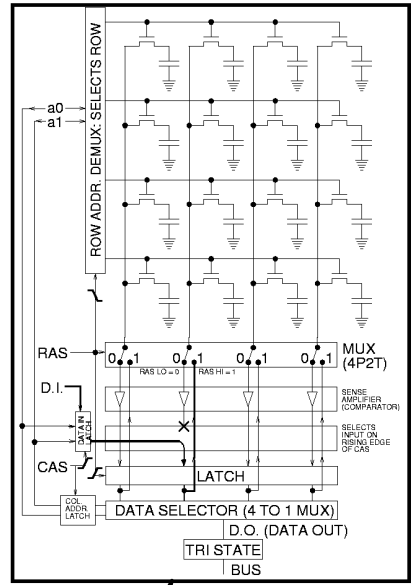
\includegraphics{image-9.png}
\caption{DRAM}
\end{figure}

La lecture des bits se fait sous forme de matrice donc si on veut lire
une valeur, on lit en réalité toute la ligne. Donc le temps pour lire 1
valeur et 64 est la même.

\begin{figure}
\centering
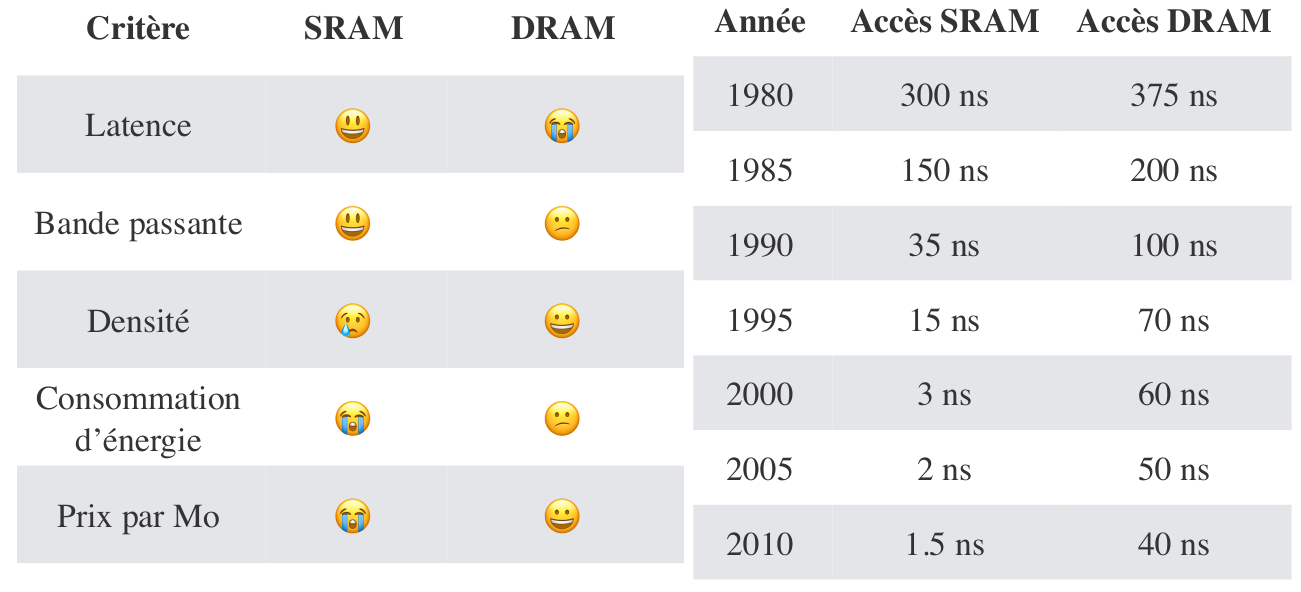
\includegraphics{image-10.png}
\caption{Reality Check}
\end{figure}

On doit donc combiner un peu de SRAM coûteuse avec de la DRAM peu chère.
On utilise la SRAM comme cache.

\subsubsection{Cache}\label{cache}

Le CPU interagit directement avec le Cache. On y conserve les données
récemment accédées.

\subsubsection{Localité}\label{localituxe9}

\paragraph{Temporelle}\label{temporelle}

On peut accéder à la même donnée se trouvant au même endroit, on va
souvent repasser dessus.

\paragraph{Localité}\label{localituxe9-1}

On va passer sur toutes les adresses car nos données sont juxtaposé.

\subsubsection{Hiérarchie}\label{hiuxe9rarchie}

(voir image)

\begin{figure}
\centering
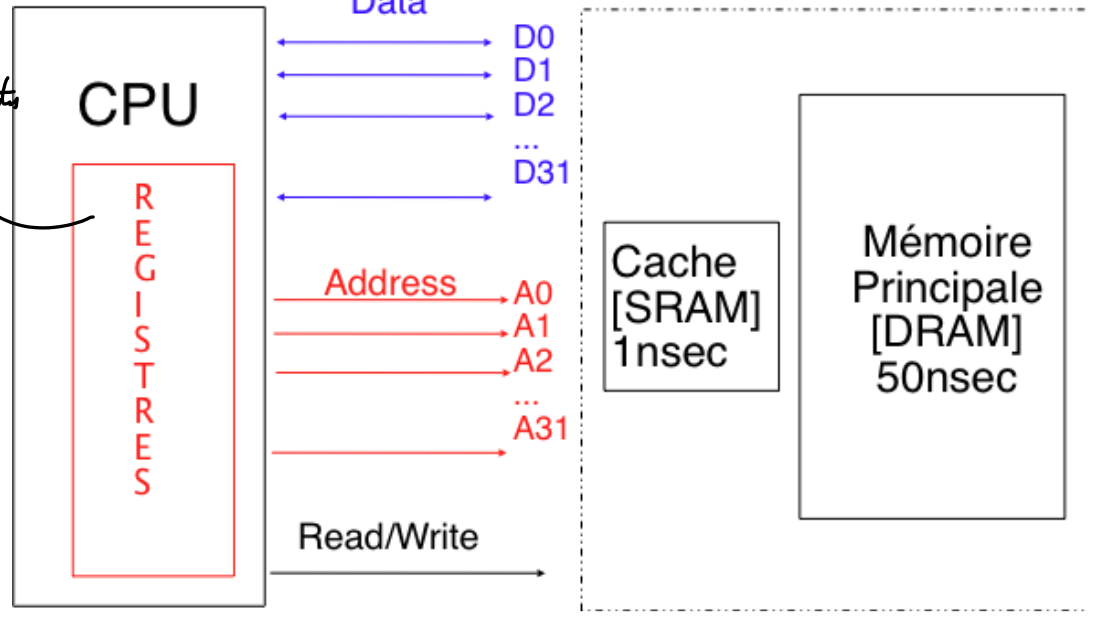
\includegraphics{image-11.png}
\caption{Hiérarchie}
\end{figure}

\subsubsection{Fonctionnement d'un
cache}\label{fonctionnement-dun-cache}

\paragraph{Lecture}\label{lecture}

On va lire l'octet à une adresse spécifique. Si cette adresse se trouve
déjà en cache on va lire l'adresse depuis le cache.

Sinon, la mémoire cache va récupérer une copie de la mémoire à cette
adresse. On a donc toute la granularité donc 64 octets ! On sauvegarde
le tout dans le cache.

\paragraph{Écriture}\label{uxe9criture}

Si on veut écrire \texttt{A}, on va regarder si on a l'adresse de
destination en cache. On écrit directement dans le cache ou bien on doit
récupérer depuis la mémoire.

\begin{enumerate}
\def\labelenumi{\arabic{enumi}.}
\tightlist
\item
  \textbf{Write through}: écriture immédiate.
\item
  \textbf{Write back}: on écrit au moment où la ligne de cache est
  retirée du cache.
\end{enumerate}

\paragraph{Réalité}\label{ruxe9alituxe9}

On a dans un processeur 3 niveaux de caches : \texttt{L1,\ L2,\ L3}

\subsection{Jeu d'instructions IA 32}\label{jeu-dinstructions-ia-32}

Ce jeu d'instructions est 32 bits ! (donc max 4 Go de mémoire).

\subsubsection{Registres}\label{registres}

On a 8 registres génériques de \textbf{32 bits}:

\begin{itemize}
\tightlist
\item
  \texttt{EAX}
\item
  \texttt{EBX}
\item
  \texttt{ECX}
\item
  \texttt{EDX}
\item
  \texttt{ESI}
\item
  \texttt{EDI}
\item
  \texttt{EBP}: gère la pile
\item
  \texttt{ESP}: gère la pile
\end{itemize}

On a 1 registres qui stocke le compteur de programme:

\begin{itemize}
\tightlist
\item
  \texttt{EIP}
\end{itemize}

On a également des registres pour traiter les floats et double.

\subsubsection{Types de données}\label{types-de-donnuxe9es}

\begin{longtable}[]{@{}ccc@{}}
\toprule\noalign{}
Type & Taille (octets) & Suffixe assembleur \\
\midrule\noalign{}
\endhead
\bottomrule\noalign{}
\endlastfoot
\texttt{char} & 1 & b \\
\texttt{short} & 2 & w \\
\texttt{int} & 4 & l \\
\texttt{long\ int} & 4 & l \\
\texttt{void\ *} & 4 & l \\
\end{longtable}

\subsubsection{Instructions}\label{instructions}

\begin{longtable}[]{@{}
  >{\centering\arraybackslash}p{(\columnwidth - 4\tabcolsep) * \real{0.1798}}
  >{\centering\arraybackslash}p{(\columnwidth - 4\tabcolsep) * \real{0.1236}}
  >{\centering\arraybackslash}p{(\columnwidth - 4\tabcolsep) * \real{0.6966}}@{}}
\toprule\noalign{}
\begin{minipage}[b]{\linewidth}\centering
Fonctions
\end{minipage} & \begin{minipage}[b]{\linewidth}\centering
Variantes
\end{minipage} & \begin{minipage}[b]{\linewidth}\centering
Explications
\end{minipage} \\
\midrule\noalign{}
\endhead
\bottomrule\noalign{}
\endlastfoot
\texttt{mov} & \texttt{movb} & \texttt{movb\ src,\ dest}: déplace de
\texttt{src} vers \texttt{dest} pour taille 1 \\
& \texttt{movw} & \texttt{movb\ src,\ dest}: déplace de \texttt{src}
vers \texttt{dest} pour taille 2 \\
& \texttt{movl} & \texttt{movb\ src,\ dest}: déplace de \texttt{src}
vers \texttt{dest} pour taille 4 \\
\texttt{inc} & \texttt{b},\texttt{w},\texttt{l} & Incrémente la
valeur \\
\texttt{dec} & \texttt{b},\texttt{w},\texttt{l} & Décrémente la
valeur \\
\texttt{not} & \texttt{b},\texttt{w},\texttt{l} & Négation \\
\texttt{add} & \texttt{b},\texttt{w},\texttt{l} &
\texttt{add\ addition,\ dest}: ajoute à dest addition \\
\texttt{sub} & \texttt{b},\texttt{w},\texttt{l} &
\texttt{sub\ soustraction,\ dest}: soustrait à dest soustraction \\
\texttt{mul} & \texttt{b},\texttt{w},\texttt{l} & Même chose que pour
sub et add, \texttt{imul} pour les nombres signés \\
\texttt{div} & \texttt{b},\texttt{w},\texttt{l} & Division d'entiers
non-signés \\
\texttt{shl} \& \texttt{shr} & \texttt{b},\texttt{w},\texttt{l} & Shift
vers la gauche et la droite (utile en binaire) \\
\texttt{or}/\texttt{xor}/\texttt{and} & \texttt{b},\texttt{w},\texttt{l}
& Opération logique binaires avec résultat dans \texttt{dist} \\
\end{longtable}

\subsubsection{Modes d'adressage}\label{modes-dadressage}

Pour spécifier un registre, on utilise \texttt{\%eax} pour spécifier le
registre \texttt{EAX}. Pour écrire une valeur dans un registre, on fait
\texttt{\$123} pour écrire \texttt{123}.

\begin{Shaded}
\begin{Highlighting}[]
\NormalTok{movl $123, \%eax ; écris dans le registre eax }
\end{Highlighting}
\end{Shaded}

On peut faire une référence \textbf{absolue}. C'est-à-dire faire
\texttt{movl\ 0x04,\ \%eax} pour mettre dans \texttt{eax} la valeur se
trouvant à l'adresse \texttt{0x04}.

On peut être \textbf{indirect}. On peut spécifier un registre qui
contient une adresse.

\begin{Shaded}
\begin{Highlighting}[]
\NormalTok{movl (\%eax), \%ecx   ; écris dans ecx ce qui se trouve dans le registre eax.}
\end{Highlighting}
\end{Shaded}

On peut faire de l'\textbf{indirect avec base et déplacement}. On accède
à une adresse + ou - la valeur donnée. On fait \texttt{D(\%reg)} qui
permet de bouger l'adresse de D.

\begin{Shaded}
\begin{Highlighting}[]
\NormalTok{movl $0x08, \%eax    ; place la valeur 0x08 dans \%eax}
\NormalTok{movl 0(\%eax), \%ecx  ; place la valeur (0xFF) se trouvant à l\textquotesingle{}adresse}
\NormalTok{                    ; 0x08= (0x08+0) dans le registre \%ecx}
\NormalTok{movl 4(\%eax), \%ecx  ; place la valeur (0x10) se trouvant à l\textquotesingle{}adresse}
\NormalTok{                    ; 0x0C (0x08+4) dans le registre \%ecx}
\NormalTok{movl {-}8(\%eax), \%ecx ; place la valeur (0x04) se trouvant à l\textquotesingle{}adresse}
\NormalTok{                    ; 0x00 (0x08{-}8) dans le registre \%ecx}
\end{Highlighting}
\end{Shaded}

\subsubsection{\texorpdfstring{Registre de drapeaux
\texttt{eflags}}{Registre de drapeaux eflags}}\label{registre-de-drapeaux-eflags}

On a un registre spécial \texttt{eflags} qui contient des bits
``drapeau'' qui est mis à jour à l'exécution des instructions.

\begin{itemize}
\tightlist
\item
  \textbf{ZF}: indique si le résultat de la dernière opération est = à
  0.
\item
  \textbf{SF}: indique si le résultat de la dernière opération est
  \textless{} à 0.
\item
  \textbf{CF}: indique si le résultat de la dernière opération
  arithmétique \textbf{non-signé} requiert plus de 32 bits.
\item
  \textbf{OF}: indique si le résultat de la dernière opération
  arithmétique \textbf{signé} requiert plus de 32 bits.
\end{itemize}

Ce registre se met à jour mais certaines opérations ne vont pas stocker
le résultat:

\begin{itemize}
\tightlist
\item
  \texttt{cmp}: équivalent de \texttt{sub}
\item
  \texttt{test}: équivalent de \texttt{and}
\end{itemize}

Pour récupérer la valeur des drapeaux on utilise \texttt{set}:

\begin{itemize}
\tightlist
\item
  \texttt{sete}: \textbf{ZF}
\item
  \texttt{sets}: \textbf{SF}
\item
  \texttt{setg}: \texttt{\textasciitilde{}SF\ \&\ ZF} en gérant
  dépassement test\textgreater{}
\item
  \texttt{setl}: \textbf{SF} et gérant le dépassement test\textless=
\end{itemize}

\paragraph{Exemples}\label{exemples}

Jetez un œil au
\href{https://sites.uclouvain.be/SystInfo/notes/Theorie/Assembleur/memory.html}{syllabus}.

\subsubsection{Saut}\label{saut}

On va modifier la valeur du \textbf{compteur de programme}
\texttt{\%eip}.

\paragraph{Inconditionnel}\label{inconditionnel}

On fait simplement \texttt{jmp\ {[}etiquette{]}}. On va donc sauter
jusqu'à une étiquette. On peut aussi sauter à une adresse mémoire via
\texttt{jmp\ *\%eax} (saute à l'instruction se trouvant à l'adresse
mémoire dans EAX).

\paragraph{Conditionnel}\label{conditionnel}

La comparaison compare avec la dernière valeur en référence.

\begin{itemize}
\tightlist
\item
  \texttt{je}: Saut si égal
\item
  \texttt{js}: Saut si négatif
\item
  \texttt{jg}: Saut si strictement supérieur à
\item
  \texttt{jge}: Saut si supérieur ou égal à
\item
  \texttt{jl}: Saut si strictement inférieur à
\item
  \texttt{jle}: Saut si inférieur ou égal à
\end{itemize}

Pour les négations, on rajoute un \texttt{n} après \texttt{j}.

\subsubsection{Manipulation de la Pile}\label{manipulation-de-la-pile}

Comme dit plus haut, la pile est stocké dans le registre \texttt{\%esp}.

\paragraph{Opérations}\label{opuxe9rations}

\begin{itemize}
\tightlist
\item
  \texttt{pushl\ \%reg}: place le contenu \texttt{\%reg} au somment de
  la pile. Décrémente la taille du registre \texttt{\%esp} de 4.
\item
  \texttt{popl\ \%reg}: retire le mot de 32 bits du sommet de la pile et
  le place dans \texttt{\%reg}. Incrémente la taille du registre
  \texttt{\%esp} de 4.
\end{itemize}

\subsubsection{Fonctions}\label{fonctions}

On a comme en Oz des procédures qui sont des fonctions sans valeur de
retour.

\paragraph{Appel}\label{appel}

\begin{enumerate}
\def\labelenumi{\arabic{enumi}.}
\tightlist
\item
  Sauver l'adresse de l'instruction qui suit l'appel de fonction
\item
  Positionner le compteur de programme à la première instruction de la
  fonction appelée
\item
  Exécuter la fonction
\item
  Positionner le compteur de programme à l'adresse qui suit l'appel,
  précédemment sauvée
\end{enumerate}

L'instruction \texttt{call} combine l'étape 1 et 2. \texttt{ret} réalise
l'étape 4. À savoir que \texttt{call} et \texttt{ret} modifie la pile
(donc \texttt{\%esp}).

\begin{Shaded}
\begin{Highlighting}[]
\NormalTok{increase:     ; étiquette de la première instruction}
\NormalTok{            movl  g,  \%eax}
\NormalTok{            addl  h,  \%eax}
\NormalTok{            movl  \%eax, g}
\NormalTok{            ret}
\NormalTok{init\_g: }
\NormalTok{            movl  $1252,  g}
\NormalTok{            ret}
\NormalTok{main: }
\NormalTok{            (...)}
\NormalTok{            calll init\_g}
\NormalTok{A\_init\_g:   calll increase}
\NormalTok{A\_increase: movl  $0, \%eax}
\NormalTok{            addl  $12, \%esp}
\NormalTok{            ret}
\NormalTok{g:}
\NormalTok{      .long 0}
\NormalTok{h:}
\NormalTok{      .long 2}
\end{Highlighting}
\end{Shaded}

\paragraph{Avec Arguments}\label{avec-arguments}

On place les arguments dans la pile. On passe donc les arguments par
\textbf{valeur}. On met donc l'adresse de retour sur le sommet de la
pile puis le premier, second, \ldots{}

Pour modifier les registres \texttt{\%eax}, \texttt{\%ecx} et
\texttt{\%edx}, il faut faire une copie de sauvegarde.

Pour modifier les registres \texttt{\%ebx}, \texttt{\%edi} et
\texttt{\%esi}, il faut copier puis restaurer. (qu'un convention)

\paragraph{Valeur de Retour}\label{valeur-de-retour}

On stocke les valeurs de retour dans le registre \texttt{\%eax} par
convention.

\href{../README.md}{\textless--}

\begin{center}\rule{0.5\linewidth}{0.5pt}\end{center}

\section{Cours 5}\label{cours-5}

\begin{itemize}
\tightlist
\item
  \hyperref[cours-5]{Cours 5}

  \begin{itemize}
  \tightlist
  \item
    \hyperref[service]{Service}

    \begin{itemize}
    \tightlist
    \item
      \hyperref[interface]{Interface}
    \item
      \hyperref[services-aux-concepteurs-dapplications]{Services aux
      concepteurs d'applications}
    \item
      \hyperref[services-aux-applications]{Services aux applications}
    \item
      \hyperref[accuxe8s-aux-services-du-se]{Accès aux services du SE}
    \end{itemize}
  \item
    \hyperref[architecture-des-systuxe8mes-dexploitation]{Architecture
    des systèmes d'exploitation}

    \begin{itemize}
    \tightlist
    \item
      \hyperref[objectifs-et-contraintes-de-mise-en-oeuvre-dun-se]{Objectifs
      et contraintes de mise en oeuvre d'un SE}
    \item
      \hyperref[ms-dos]{MS-DOS}
    \item
      \hyperref[unix]{UNIX}
    \item
      \hyperref[macro--et-micro-noyaux]{Macro- et Micro-noyaux}
    \item
      \hyperref[fiabilituxe9-des-se]{Fiabilité des SE}
    \item
      \hyperref[duxe9marrage-du-se]{Démarrage du SE}
    \end{itemize}
  \end{itemize}
\end{itemize}

\subsection{Service}\label{service}

Un système d'exploitation fournit des services aux utilisateurs (aussi
distant), aux développeurs et programmes qui s'exécutent.

\subsubsection{Interface}\label{interface}

\begin{itemize}
\tightlist
\item
  Interface utilisateur: GUI ou terminal
\item
  Interface de traitement par lot: comme Inginious, on a un ensemble de
  tâches qui s'exécutent groupe par groupe. (punch card)
\end{itemize}

On retrouve la dernière interface sur les HPC et autres types de super
computer.

\paragraph{Sous linux}\label{sous-linux}

On a un système pour le batch (traitement par lot).

\begin{itemize}
\tightlist
\item
  \texttt{at}: lance une commande à un moment spécifique.
\item
  \texttt{crontab}: gérer des tâches récurrentes.
\end{itemize}

\subsubsection{Services aux concepteurs
d'applications}\label{services-aux-concepteurs-dapplications}

On facilite le déploiement d'applications sur d'autres systèmes que
celui de la machine du dev via: - \textbf{Linker}: Assemble différents
fichiers \emph{objets} en un \emph{exécutable unique} - \texttt{ld} sur
Linux - \texttt{-static} avec \texttt{gcc} pour avoir l'ensemble des
libraires - \textbf{Loader}: au démarrage d'un programme. -
\texttt{ld.so} libraire et support du kernel Linux 1. Initialise
l'espace mémoire 2. Pré-charge les segments text, data, environment 3.
Localiser et charger les libraires dynamiques

Il peut aussi gérer les erreurs. ex: \emph{memory dump} pour avoir
l'état de la mémoire avant le crash. Ce \emph{memory dump} peut être
déclenché si on fait une division par 0 ou accès non autorisé à certains
segments de la mémoire.

On peut aussi facilement débugger via \texttt{gdb} et ses breakpoints.
Les breakpoints sont en réalité des \emph{trap} qui fait une
interruption logicielle !

\subsubsection{Services aux
applications}\label{services-aux-applications}

Le SE gère les entrées sorties mais il y a quelques règles: - Une app
\textbf{ne peut pas} envoyer d'instructions aux gestionnaires de
périphériques - \textbf{Ne peut pas} traiter les interruptions -
Hétérogénéité des périphériques eux-mêmes - SE fournit une abstraction
unique pour une \emph{classe} de périphérique

Un des buts du SE est de faire \textbf{correspondre} des abstractions
\emph{haut niveau} et des opérations \emph{bas niveau}. On a des drivers
qui permettent de contrôler le matériel.

Un SE va partager les ressources. Il va faire: - Maximisation de
l'utilisation - Équité d'accès - Isolation

Il fournit aussi d'autres services spécifiques: - Allocations des
ressources: - Exclusive ou non (typique des ports) - Contrôle générique
ou spécifique - Protection et contrôle d'accès

\subsubsection{Accès aux services du
SE}\label{accuxe8s-aux-services-du-se}

\begin{itemize}
\tightlist
\item
  Utilisation d'utilitaire systèmes
\item
  Appel direct des fonctions du noyau
\item
  Librairie Standard
\end{itemize}

On a une API par le noyau pour les \emph{appels système}: - A un numéro
précis - Point d'entrée unique pour accéder aux fonctions du noyau

\paragraph{Fonctionnement}\label{fonctionnement}

\begin{enumerate}
\def\labelenumi{\arabic{enumi}.}
\tightlist
\item
  Placer les arguments dans la pile
\item
  Sauvegarde l'adresse de retour sur la pile
\item
  Modifier \texttt{\%eip} pour que la prochaine instruction à exécuter
  soit notre fonction
\item
  Fonction prend ses arguments
\item
  Sauvegarde son résultat à un endroit (\texttt{\%eax} par convention en
  IA32)
\item
  Fonction récupère l'adresse de retour sur la pile et modifie
  \texttt{\%eip} pour retourner à la fonction appelante.
\end{enumerate}

\begin{figure}
\centering
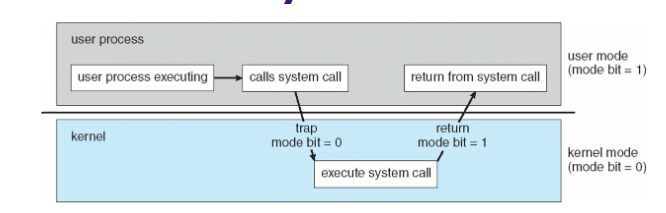
\includegraphics{image-12.png}
\caption{Alt text}
\end{figure}

On change de mode d'exécution. On change d'espace mémoire !

\paragraph{Réalisation concrète}\label{ruxe9alisation-concruxe8te}

Problème 1: placer des arguments qui seront accessibles par le noyau. On
va le mettre soit dans: - Un espace mémoire fixe dédié (data) - Sur la
pile - Registres (\texttt{\%ebx} pour premier argument puis
\texttt{\%ecx})

Problème 2: adresse de retour - Pointeur de programme sauvegardé sur la
pile. - Restauré au retour

Problème 3: appel effectif - Passer en mode protégé - Instructions
spéciales (IA32 \texttt{int\ 0x80} crée une interruption) ou simplement
\texttt{syscall}. - Point d'entrée du kernel est connu par le
processeur.

\begin{figure}
\centering
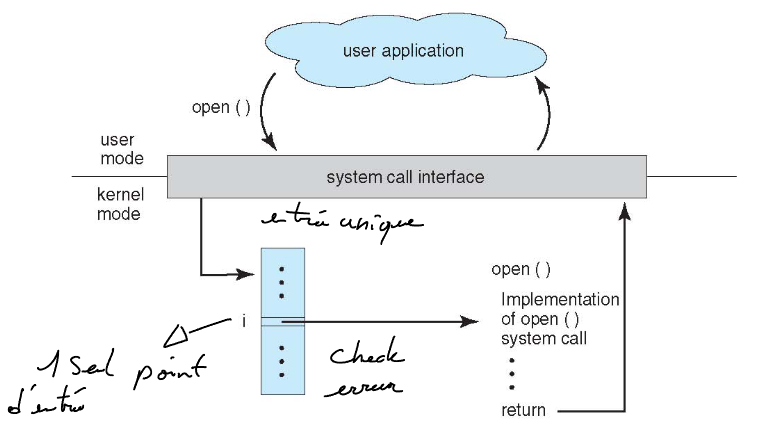
\includegraphics{image-13.png}
\caption{Alt text}
\end{figure}

Problème 4: récupération du code de retour 1. Opération autorisée et
paramètre corrects: - Résultat mis dans le registre \texttt{\%eax} -
Instruction de retour au mode utilisateur, dépile l'adresse de retour et
positionne le compteur de programme 2. Erreur ou opération non autorisée
- Positionne la variable d'environnement \texttt{errno} - Retourne aux
processus parent (ex: shell)

\paragraph{Appels systèmes}\label{appels-systuxe8mes}

\begin{itemize}
\tightlist
\item
  Librairie standard: s'exécute dans le même espace mémoire que le
  programme utilisateur. \texttt{printf(3)} va forcément utiliser
  \texttt{write(2)} ou autres opérations bas niveau.
\item
  \texttt{strace(1)} permet de tracer les appels systèmes utilisés par
  un processus
\end{itemize}

.

\begin{figure}
\centering
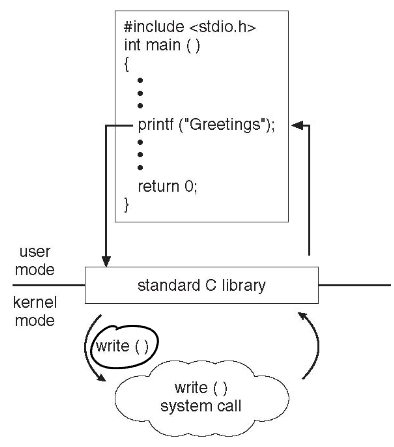
\includegraphics{image-14.png}
\caption{Alt text}
\end{figure}

\paragraph{Hello world}\label{hello-world}

\begin{Shaded}
\begin{Highlighting}[]
\PreprocessorTok{\#include }\ImportTok{\textless{}stdio.h\textgreater{}}
\PreprocessorTok{\#include }\ImportTok{\textless{}stdlib.h\textgreater{}}

\DataTypeTok{int}\NormalTok{ main}\OperatorTok{(}\DataTypeTok{int}\NormalTok{ argc}\OperatorTok{,} \DataTypeTok{char} \OperatorTok{*}\NormalTok{argv}\OperatorTok{[])\{}
\NormalTok{   printf}\OperatorTok{(}\StringTok{"Hello, world! }\SpecialCharTok{\%d\textbackslash{}n}\StringTok{"}\OperatorTok{,}\KeywordTok{sizeof}\OperatorTok{(}\DataTypeTok{int}\OperatorTok{));}
   \ControlFlowTok{return}\NormalTok{ EXIT\_SUCCESS}\OperatorTok{;}
\OperatorTok{\}}
\end{Highlighting}
\end{Shaded}

Traduction:

\begin{verbatim}
$ strace ./helloworld_s
execve("./helloworld_s", ["./helloworld_s"], [/* 21 vars */]) = 0
uname({sys="Linux", node="precise32", ...}) = 0
brk(0)                                  = 0x9e8b000
brk(0x9e8bd40)                          = 0x9e8bd40
set_thread_area({entry_number:-1 -> 6, base_addr:0x9e8b840, limit:1048575, seg_32bit:1, 
contents:0, read_exec_only:0, limit_in_pages:1, seg_not_present:0, useable:1}) = 0
brk(0x9eacd40)                          = 0x9eacd40
brk(0x9ead000)                          = 0x9ead000
fstat64(1, {st_mode=S_IFCHR|0620, st_rdev=makedev(136, 0), ...}) = 0
mmap2(NULL, 4096, PROT_READ|PROT_WRITE, MAP_PRIVATE|MAP_ANONYMOUS, -1, 0) = 0xb778a000
write(1, "Hello, world! 4\n", 16Hello, world! 4
)       = 16
exit_group(0)                           = ?
\end{verbatim}

\subsection{Architecture des systèmes
d'exploitation}\label{architecture-des-systuxe8mes-dexploitation}

\begin{figure}
\centering
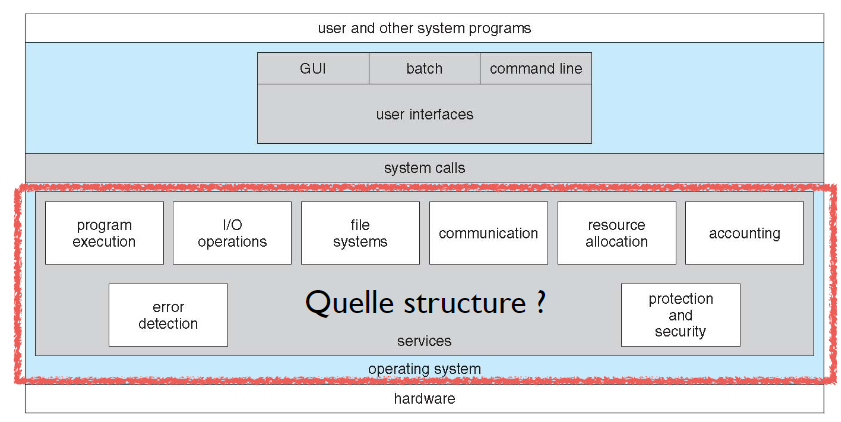
\includegraphics{image-15.png}
\caption{Alt text}
\end{figure}

\subsubsection{Objectifs et contraintes de mise en oeuvre d'un
SE}\label{objectifs-et-contraintes-de-mise-en-oeuvre-dun-se}

\begin{itemize}
\tightlist
\item
  Pas de modèle unique et parfait
\item
  Contraintes et objectifs:

  \begin{itemize}
  \tightlist
  \item
    Contraintes du matériel
  \item
    Performance et coût d'implémentation
  \item
    Consommation de ressources
  \item
    Facilité d'évolution et d'adaptation
  \item
    Facilité de maintenance et d'atteinte de fiabilité
  \end{itemize}
\end{itemize}

\subsubsection{MS-DOS}\label{ms-dos}

SE des systèmes \emph{IBM-PC} pas basé sur UNIX, c'est Microsoft.

Objectifs: - Mono-utilisateur et mono-application (Pas de temps partagé)
- Visant des processeurs \textbf{ne supportant pas} les modes
utilisateur/protégé (Pas d'isolation) - Contrainte forte sur
l'utilisation de la mémoire (coutait extrêmement cher à l'époque)

Système avec une vision \textbf{monolithique} pour éviter de consommer
trop de mémoire.

\begin{figure}
\centering
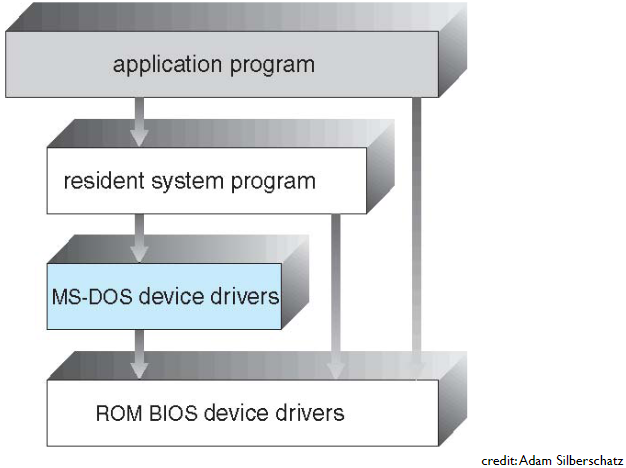
\includegraphics{image-16.png}
\caption{Alt text}
\end{figure}

\begin{figure}
\centering
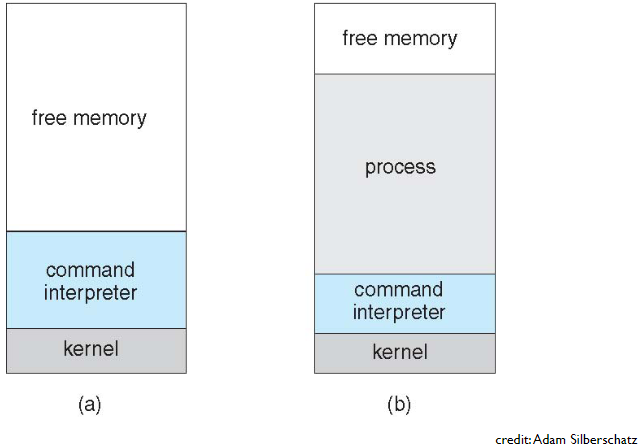
\includegraphics{image-17.png}
\caption{Alt text}
\end{figure}

\subsubsection{UNIX}\label{unix}

\paragraph{Monolithe}\label{monolithe}

Plus vieux que \hyperref[ms-dos]{MS-DOS} mais pensé pour des ordinateurs
à plus grande capacité. - Multi utilisateur et temps partagé -
Processeur supportant les deux modes - Séparation claire entre
\emph{noyau} et \emph{programmes utilisateurs}

Organisation originelle: \emph{monolithe}: - 1 seul programme sur 1
seule couche, met en oeuvre tous les appels systèmes - Difficile à
étendre, adapter, débugger

\begin{figure}
\centering
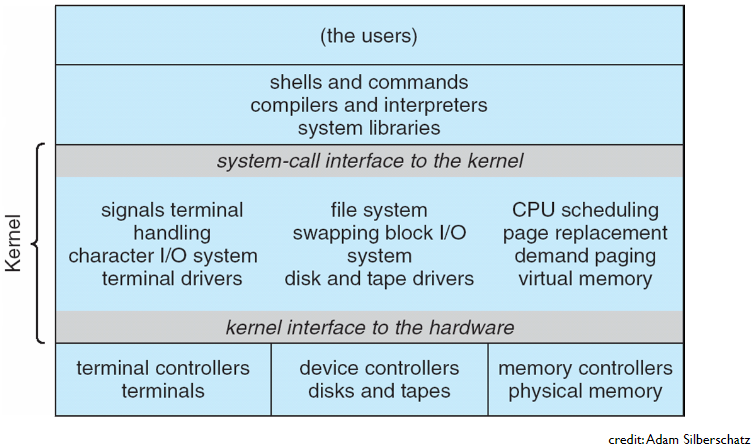
\includegraphics{image-18.png}
\caption{Alt text}
\end{figure}

\paragraph{Couches}\label{couches}

On va rajouter de la structure pour pallier aux soucis lié à
\hyperref[monolithe]{unix monolithique}

Les couches: 1. Matériel 2. Drivers de périphériques 3. Abstractions des
plus en plus haut niveau, jusqu'aux appels systèmes 4. Interface
utilisateur

\begin{figure}
\centering
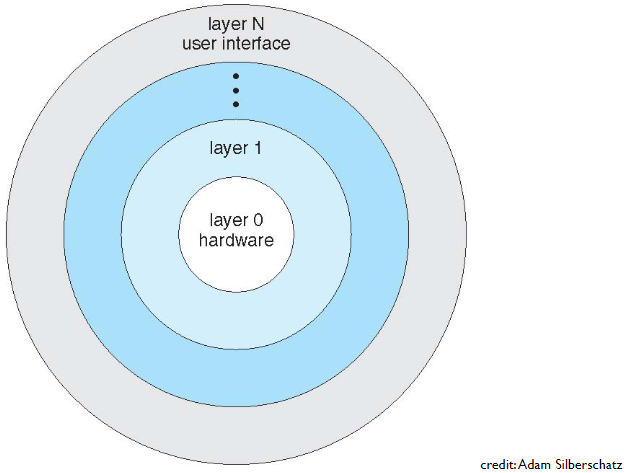
\includegraphics{image-19.png}
\caption{Alt text}
\end{figure}

Il y a des avantages et inconvénients !

Avantages: - Isolations des fonctionnalités - Facilité de portage

Inconvénients: - Surcoût à l'exécution des appels système - Difficile de
décider d'une structure purement hiérarchique. - Il y a une
interdépendance entre les fonctions du SE

\paragraph{Structure en Modules}\label{structure-en-modules}

\begin{figure}
\centering
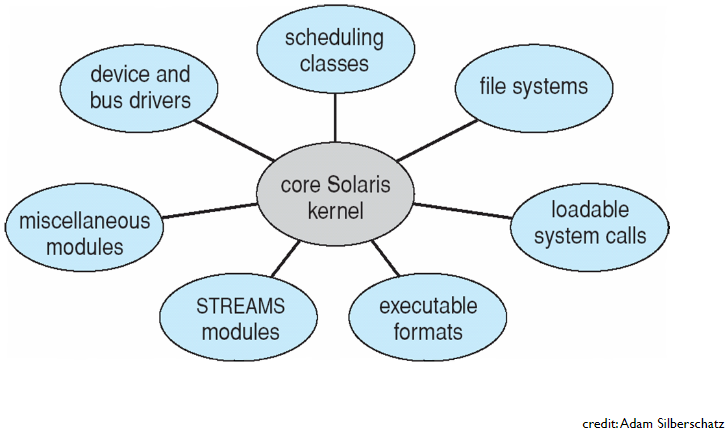
\includegraphics{image-20.png}
\caption{Alt text}
\end{figure}

Utilisé le plus souvent: Linux, Solaris, Windows

On a un coeur qui est un monolithe ou qui a peu de couche. - Gestion bas
niveau de la mémoire - Gestion des processus

Le reste est sous forme de modules: - Chargés et décharges de l'espace
mémoire du noyau \emph{dynamiquement} - Seulement lorsque nécessaire -
Ex: quand on met une clé usb. Va charger \texttt{exFAT} si clé venant de
Windows

Avantages: - Spécialisation d'une SE pour un environnement donné: -
Versatilité de Linux - Interactions possibles entre les modules en
conservant la séparation de code et de mémoire. - Analogie possible avec
programmation orientée objet

Inconvénients: - Surcoût (négligeable sur les systèmes modernes) -
Intégration de modules écrits par des tiers dans l'espace mémoire du
noyau - potentiels bugs et fautes

Gestions des modules sous Linux (seulement si \texttt{root}): -
\texttt{lsmod}: liste les modules présents - \texttt{modprobe}:
ajoute/supprime un module - \texttt{modinfo}: information sur un module

\subsubsection{Macro- et Micro-noyaux}\label{macro--et-micro-noyaux}

\paragraph{Macro-noyaux}\label{macro-noyaux}

Tous les modes précédents placent l'intégralité des fonctions du SE dans
le noyau. - Toutes s'exécutent en mode protégé - Accès complet à la
mémoire et aux instructions sensibles - Crash du module = \textbf{crash
du système}

Le kernel est en pérille, corruption des données, faille pour les
hackers.

\paragraph{Micro-noyaux}\label{micro-noyaux}

Séparation entre un noyau minimaliste - Gestion basique de la mémoire -
Gestion des processus légers (threads) - Gestion de la communication
entre processus (IPC)

Le reste est mis en oeuvre par des processus en mode utilisateur (même
les drivers)

Réduit les bugs de modules et évitent les crash complets tout en gardant
les propriétés d'isolation.

\begin{figure}
\centering
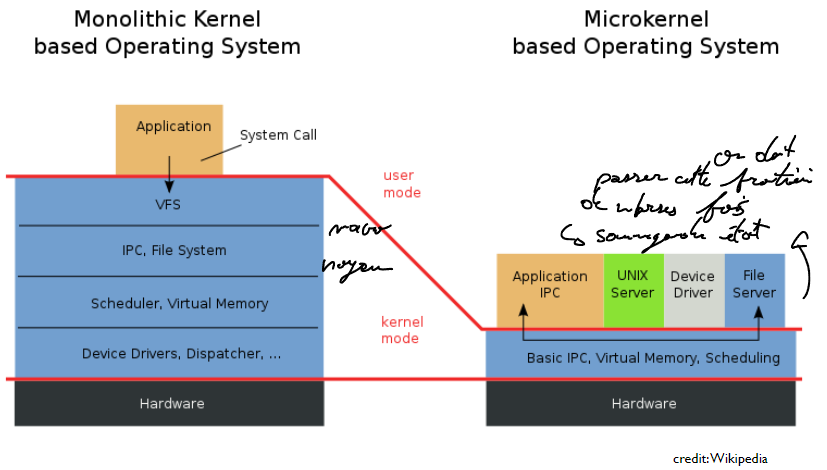
\includegraphics{image-21.png}
\caption{Alt text}
\end{figure}

Inconvénients: - En macro: appel de module dans un même espace mémoire
donc très rapide. En micro: il faut faire des appels systèmes - Copie de
l'argument de l'appelant vers le noyau - Copie dans l'espace mémoire de
l'appelé - Changement de contexte (sauvegarde du contexte et
restauration\ldots) - \ldots{} et rebelote dans l'autre sens pour la
valeur de retour

Donc on a longtemps abandonnés les micro-noyaux (abandon dans Windows
NT) MAIS: - Progrès sensibles dans la mise en oeuvre des appels systèmes
- Passage de message en mode zero-copy - Mac OS et iOS proche d'un
micro-noyau

\subsubsection{Fiabilité des SE}\label{fiabilituxe9-des-se}

Souvent beaucoup de temps nécessaires pour corriger des fautes.
Énormément de fautes dans les drivers et compliqués à débugger et
trouver parfois.

\paragraph{Certification formelle}\label{certification-formelle}

Pour les systèmes embarqués critiques on réalise des
\textbf{spécification formelle}. On modélise \emph{mathématiquement}
qu'un système est fiable. C'est le cas pour seL4. Mais seulement
possible si le code est petit.

\subsubsection{Démarrage du SE}\label{duxe9marrage-du-se}

Démarrage et reset de la machine: interruption de mise à zéro du
processeur. 2 phases:

\begin{enumerate}
\def\labelenumi{\arabic{enumi}.}
\tightlist
\item
  Programme de démarrage (bootstrap) stocké dans une ROM. Charge ainsi
  le bootloader
\item
  Bootloader lit les systèmes de fichiers pour charger l'image du noyau
  en mémoire (\texttt{/boot/vmlinuz-3.12.0-32-generic}) en gros le GRUB.
\end{enumerate}

\begin{center}\rule{0.5\linewidth}{0.5pt}\end{center}

\href{../README.md}{\textless--}

\section{Cours 6}\label{cours-6}

\subsection{Course à la performance}\label{course-uxe0-la-performance}

Selon la loi empirique de Moore, tous les 18 mois, la quantité de
transistor sur \(1\) \(cm^2\) double.

\subsubsection{Horloge}\label{horloge}

On sait que les processeurs fonctionnent sur des cycles régulés par
l'horloge. On voit apparaître un plateau vers 2001 pour les fréquences
d'horloge.

\paragraph{Raison}\label{raison}

\begin{itemize}
\tightlist
\item
  \emph{Memory Wall}: la différence entre fréquence CPU et RAM est trop
  importante. Demande plus de cache mais c'est cher
\item
  \emph{Instruction-Level Parallelism}: Même si possible de paralléliser
  les processus, on reste limité par les instructions bas niveaux.
\item
  \emph{Power Wall}: + de fréquence = + de consommation d'énergie = + de
  dissipation thermique. Cela devient compliqué à refroidir.
\end{itemize}

\subsubsection{Augmentation des
performances}\label{augmentation-des-performances}

\begin{figure}
\centering
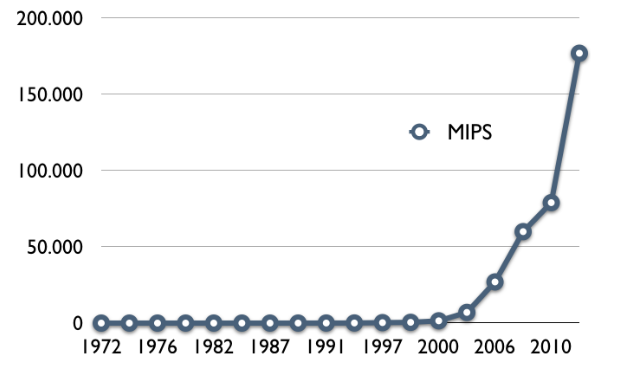
\includegraphics{image-22.png}
\caption{Alt text}
\end{figure}

On voit bien que le \emph{Millions d'Instructions par Seconde} augmente
tout de même.

Ces résultats sont démontrés via des \textbf{benchmarks standardisés}.
(SPEC = organisation de standardisation de benchmarks)

\paragraph{Multi-coeurs}\label{multi-coeurs}

C'est grâce au multi-coeurs ! Le nombre de transistor augmente mais la
fréquence est stable donc le nombre d'instructions par seconde augmente.

On peut ainsi avoir plusieurs \textbf{threads} qui s'exécutent en
simultanée.

\begin{figure}
\centering
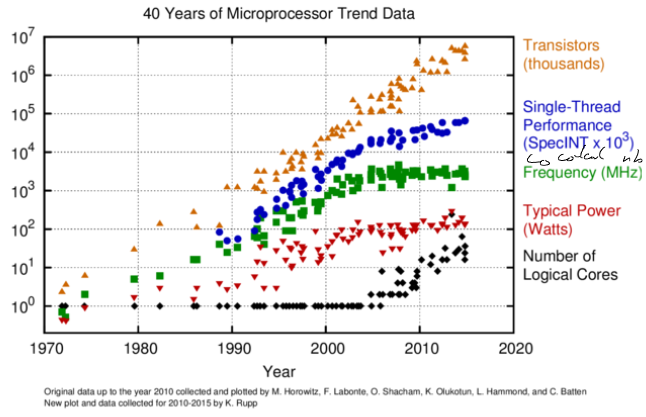
\includegraphics{image-23.png}
\caption{Alt text}
\end{figure}

On ne remplit pas totalement tous les coeurs via un seul programme car
il manque de parallélisme d'instruction (ILP).

Les ressources du coeur sont partagées entre 2 fils d'instructions
distincts:

\begin{itemize}
\tightlist
\item
  \textbf{SMT}: \emph{Simultaneous Multi-Threading}
\item
  32 fils par coeur sur certains CPU
\item
  2 fils par coeur souvent (\emph{Hyperthreading})
\end{itemize}

Un peu inférieur: 16 threads \textless{} 16 coeurs

\subsection{Threads}\label{threads}

\subsubsection{Qu'est-ce qu'un thread ?}\label{quest-ce-quun-thread}

Un threads est donc:

\begin{enumerate}
\def\labelenumi{\arabic{enumi}.}
\tightlist
\item
  Instructions à exécuter (text)
\item
  Mémoires contenant les données manipulées (\emph{data, heap, stack})
\item
  Registres du CPU (son état actuel)
\end{enumerate}

\subsubsection{Mise en oeuvre (POSIX)}\label{mise-en-oeuvre-posix}

Avec les threads POSIX: \emph{threads du programme utilisateur = threads
ordonnancé sur les coeurs par le noyau}. En gros le gain des threads
POSIX se fait sentir jusqu'à ce que le nombre de threads du programme
atteignent ceux du CPU (cfr: Projet 3).

\paragraph{Utilisation}\label{utilisation}

On utilise la libraire \texttt{pthreads(7)} et à la compilation on doit
passer le flag \texttt{-lpthread} à gcc.

\begin{Shaded}
\begin{Highlighting}[]
\PreprocessorTok{\#include }\ImportTok{\textless{}pthread.h\textgreater{}}

\DataTypeTok{int}\NormalTok{ pthread\_create}\OperatorTok{(}\NormalTok{pthread\_t }\OperatorTok{*}\DataTypeTok{restrict}\NormalTok{ thread}\OperatorTok{,}
                   \DataTypeTok{const}\NormalTok{ pthread\_attr\_t }\OperatorTok{*}\DataTypeTok{restrict}\NormalTok{ attr}\OperatorTok{,}
                   \DataTypeTok{void} \OperatorTok{*(*}\NormalTok{start\_routine}\OperatorTok{)(}\DataTypeTok{void} \OperatorTok{*),}
                   \DataTypeTok{void} \OperatorTok{*}\DataTypeTok{restrict}\NormalTok{ arg}\OperatorTok{);}
\end{Highlighting}
\end{Shaded}

\begin{itemize}
\tightlist
\item
  \texttt{thread}: structure de donnée provenant de \texttt{pthread.h}
\item
  attributs: \texttt{NULL} par défaut
\item
  \texttt{start\_routine}: pointeur sur la fonction, point de départ du
  thread
\item
  \texttt{arg}: arguments à passer à notre fonction de
  \texttt{start\_routine}
\end{itemize}

Retourne \(0\) si aucune erreur.

\paragraph{Récupérer la valeur de
retour}\label{ruxe9cupuxe9rer-la-valeur-de-retour}

\begin{Shaded}
\begin{Highlighting}[]
\PreprocessorTok{\#include }\ImportTok{\textless{}pthread.h\textgreater{}}

\DataTypeTok{int}\NormalTok{ pthread\_join}\OperatorTok{(}\NormalTok{pthread\_t thread}\OperatorTok{,} \DataTypeTok{void} \OperatorTok{**}\NormalTok{value\_ptr}\OperatorTok{);}
\end{Highlighting}
\end{Shaded}

\begin{itemize}
\tightlist
\item
  \texttt{thread}: thread concerné.
\item
  \texttt{value\_ptr}: pointeur où on va récupérer la valeur.
\end{itemize}

\texttt{pthread\_join} ne retourne qu'à la terminaison du thread. Donc
on attend jusqu'à la fin de son exécution.

\paragraph{Fonctionnement}\label{fonctionnement}

Au moment d'exécuter \texttt{pthread\_create} la pile du thread est
créée et la valeur de l'argument y est copié. Donc on doit s'assurer que
le pointeur passé soit toujours valide à n'importe quel moment. Moment
de l'exécution du thread inconnu.

Dans un thread, il a un nouveau stack et contexte (\%esp, \%eip,
registres). Cependant il utilise le heap, les données statiques et le
text du processus principal.

\subsubsection{Communication entre
thread}\label{communication-entre-thread}

On va utiliser des locks pour pouvoir accéder à des variables globales
sans se marcher dessus.

On doit d'abord s'assurer de gérer les interruptions pour les
\textbf{changements de contexte}. On fait cela via:

\begin{itemize}
\tightlist
\item
  Appel système bloquant
\item
  Réception d'une interruption:

  \begin{itemize}
  \tightlist
  \item
    Signal électronique reçu par le processeur pour signaler la
    disponibilité d'une E/S
  \item
    Ou via un timer régulier.
  \end{itemize}
\end{itemize}

Appel bloquant comme \texttt{getchar} qui attend une entrée utilisateur.

\subsubsection{États}\label{uxe9tats}

\begin{figure}
\centering
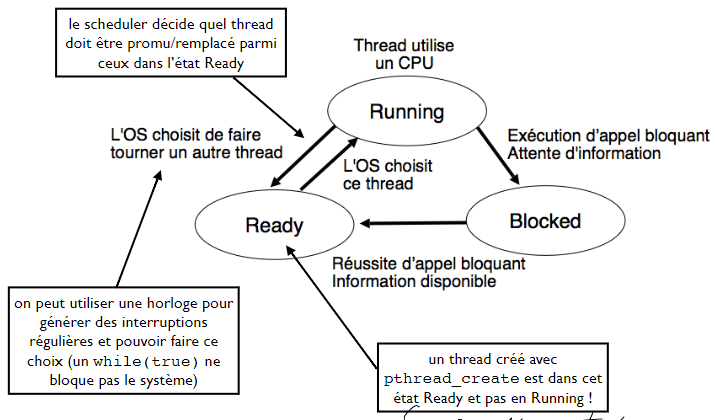
\includegraphics{image-24.png}
\caption{Alt text}
\end{figure}

\paragraph{Laisser la main}\label{laisser-la-main}

Un thread peut libérer le processeur via \texttt{pthread\_yield} pour ne
pas bloquer (appel sys bloquant \texttt{sleep}/\texttt{usleep}).

Il faut faire attention au blocage de la machine suite à l'arrêt des
entrées/sorties.

\subsubsection{MUTEX}\label{mutex}

C'est un objet qui va être \textbf{unlocked} si on peut y accéder et
\textbf{locked} si on ne peut pas. On utilise les fonctions
\texttt{lock()} et \texttt{unlock()}.

Si un thread appelle \texttt{lock()} et que le mutex est déjà bloqué,
alors le thread sera interrompu et placé en mode \textbf{Blocked}
jusqu'à ce que le mutex soit libéré. \texttt{lock()} peut créer un appel
sys bloquant.

\paragraph{Deadlock}\label{deadlock}

cela se passe quand tout se bloque à cause de mutex (cfr: 3 philosophes
3 baguettes). On peut forcer que les appels bloquants se fassent par
ordre croissant d'adresse pour éviter ce problème.

\section{Cours 7}\label{cours-7}

\subsection{Sémaphores et Compléments sur les
Threads}\label{suxe9maphores-et-compluxe9ments-sur-les-threads}

\subsubsection{Sémaphore}\label{suxe9maphore}

Une sémaphore est donc une structure qui contient: - Entier non-signé:
positif ou nul - File vers les pointeurs de threads en attente
(\emph{Blocked})

\begin{Shaded}
\begin{Highlighting}[]
\PreprocessorTok{\#include }\ImportTok{\textless{}semaphore.h\textgreater{}}\PreprocessorTok{ }
\DataTypeTok{int}\NormalTok{ sem\_init}\OperatorTok{(}\NormalTok{sem\_t }\OperatorTok{*}\NormalTok{sem}\OperatorTok{,} \DataTypeTok{int}\NormalTok{ pshared}\OperatorTok{,} \DataTypeTok{unsigned} \DataTypeTok{int}\NormalTok{ value}\OperatorTok{);} \CommentTok{// initialise avec value le nombre de place}
\CommentTok{//pshared = 0}
\DataTypeTok{int}\NormalTok{ sem\_destroy}\OperatorTok{(}\NormalTok{sem\_t }\OperatorTok{*}\NormalTok{sem}\OperatorTok{);} \CommentTok{// destruction du semaphore }
\DataTypeTok{int}\NormalTok{ sem\_wait}\OperatorTok{(}\NormalTok{sem\_t }\OperatorTok{*}\NormalTok{sem}\OperatorTok{);} \CommentTok{// Attente place}
\DataTypeTok{int}\NormalTok{ sem\_post}\OperatorTok{(}\NormalTok{sem\_t }\OperatorTok{*}\NormalTok{sem}\OperatorTok{);} \CommentTok{// Liberation place}
\end{Highlighting}
\end{Shaded}

Utile pour les problèmes de rendez-vous, producteurs-consommateurs,
lecteurs-écrivains, \ldots{}

Donc une sémaphore avec \texttt{value\ =\ 1} est une sorte de mutex.
Attention, un autre thread peut libérer notre sémaphore ce qui est
différent d'un mutex où c'est généralement le même thread appelle
\texttt{lock()} et \texttt{unlock()}.

\paragraph{Problème du Rendez-Vous}\label{probluxe8me-du-rendez-vous}

2 phases: 1. N threads s'exécutent indépendamment 2. Commence quand tous
les threads ont finit la phase 1. (on peut utiliser la structure
\texttt{pthread\_barrier\_init})

\begin{Shaded}
\begin{Highlighting}[]
\NormalTok{sem\_t rendezvous}\OperatorTok{;} \CommentTok{// Bloque les threads en attente de RDV }
\NormalTok{pthread\_mutex\_t mutex}\OperatorTok{;} \CommentTok{// Protège accès à count}
\DataTypeTok{int}\NormalTok{ count}\OperatorTok{=}\DecValTok{0}\OperatorTok{;} \CommentTok{// Nombre de threads ayant atteint le point de RDV}

\NormalTok{sem\_init}\OperatorTok{(\&}\NormalTok{rendezvous}\OperatorTok{,}\DecValTok{0}\OperatorTok{,}\DecValTok{0}\OperatorTok{)}

\NormalTok{premiere\_phase}\OperatorTok{();} 

\CommentTok{// section critique }
\NormalTok{pthread\_mutex\_lock}\OperatorTok{(\&}\NormalTok{mutex}\OperatorTok{);}\NormalTok{ count}\OperatorTok{++;} 
\ControlFlowTok{if}\OperatorTok{(}\NormalTok{count}\OperatorTok{==}\NormalTok{N}\OperatorTok{)} \OperatorTok{\{}
    \CommentTok{// tous les threads sont arrivés }
\NormalTok{    sem\_post}\OperatorTok{(\&}\NormalTok{rendezvous}\OperatorTok{);}
\OperatorTok{\}}
\NormalTok{pthread\_mutex\_unlock}\OperatorTok{(\&}\NormalTok{mutex}\OperatorTok{);} 
\CommentTok{// attente à la barrière }
\NormalTok{sem\_wait}\OperatorTok{(\&}\NormalTok{rendezvous}\OperatorTok{);}
\CommentTok{// libération d\textquotesingle{}un autre thread en attente }
\NormalTok{sem\_post}\OperatorTok{(\&}\NormalTok{rendezvous}\OperatorTok{);}

\NormalTok{seconde\_phase}\OperatorTok{();}
\end{Highlighting}
\end{Shaded}

\paragraph{Producteurs-Consommateurs}\label{producteurs-consommateurs}

On a un ensemble de threads qui produisent quelque chosent et d'autres
qui vont le consommer. Les producteurs vont donc placer leurs données
dans une zone partagée et les consommateurs vont pouvoir se servir.

\begin{Shaded}
\begin{Highlighting}[]
\CommentTok{// Initialisation }
\PreprocessorTok{\#define N }\DecValTok{10}\PreprocessorTok{ }
\CommentTok{// places dans le buffer }
\NormalTok{pthread\_mutex\_t mutex}\OperatorTok{;} 
\NormalTok{sem\_t empty}\OperatorTok{;} 
\NormalTok{sem\_t full}\OperatorTok{;}

\NormalTok{pthread\_mutex\_init}\OperatorTok{(\&}\NormalTok{mutex}\OperatorTok{,}\NormalTok{ NULL}\OperatorTok{);} 
\NormalTok{sem\_init}\OperatorTok{(\&}\NormalTok{empty}\OperatorTok{,} \DecValTok{0} \OperatorTok{,}\NormalTok{ N}\OperatorTok{);} \CommentTok{// buffer vide}
\NormalTok{sem\_init}\OperatorTok{(\&}\NormalTok{full}\OperatorTok{,} \DecValTok{0} \OperatorTok{,} \DecValTok{0}\OperatorTok{);} \CommentTok{// buffer vide}

\CommentTok{// Producteur}
\DataTypeTok{void}\NormalTok{ producer}\OperatorTok{(}\DataTypeTok{void}\OperatorTok{)} \OperatorTok{\{}
    \DataTypeTok{int}\NormalTok{ item}\OperatorTok{;} 
    \ControlFlowTok{while}\OperatorTok{(}\KeywordTok{true}\OperatorTok{)} \OperatorTok{\{}
\NormalTok{        item}\OperatorTok{=}\NormalTok{produce}\OperatorTok{(}\NormalTok{item}\OperatorTok{);} 
\NormalTok{        sem\_wait}\OperatorTok{(\&}\NormalTok{empty}\OperatorTok{);} \CommentTok{// attente d\textquotesingle{}une place libre }
\NormalTok{        pthread\_mutex\_lock}\OperatorTok{(\&}\NormalTok{mutex}\OperatorTok{);} 
        \CommentTok{// section critique }
\NormalTok{        insert\_item}\OperatorTok{();}
\NormalTok{        pthread\_mutex\_unlock}\OperatorTok{(\&}\NormalTok{mutex}\OperatorTok{);}
\NormalTok{        sem\_post}\OperatorTok{(\&}\NormalTok{full}\OperatorTok{);} \CommentTok{// une place remplie}
    \OperatorTok{\}}
\OperatorTok{\}}

\CommentTok{// Consommateur}
\DataTypeTok{void}\NormalTok{ consumer}\OperatorTok{(}\DataTypeTok{void}\OperatorTok{)} \OperatorTok{\{}
    \DataTypeTok{int}\NormalTok{ item}\OperatorTok{;} 
    \ControlFlowTok{while}\OperatorTok{(}\KeywordTok{true}\OperatorTok{)} \OperatorTok{\{}
\NormalTok{        sem\_wait}\OperatorTok{(\&}\NormalTok{full}\OperatorTok{);} \CommentTok{// attente d\textquotesingle{}une place remplie }
\NormalTok{        pthread\_mutex\_lock}\OperatorTok{(\&}\NormalTok{mutex}\OperatorTok{);} 
        \CommentTok{// section critique }
\NormalTok{        item }\OperatorTok{=}\NormalTok{ remove}\OperatorTok{(}\NormalTok{item}\OperatorTok{);}
\NormalTok{        pthread\_mutex\_unlock}\OperatorTok{(\&}\NormalTok{mutex}\OperatorTok{);}
\NormalTok{        sem\_post}\OperatorTok{(\&}\NormalTok{empty}\OperatorTok{);} \CommentTok{// une place libre}
    \OperatorTok{\}}
\OperatorTok{\}}
\end{Highlighting}
\end{Shaded}

\paragraph{Reader-writers}\label{reader-writers}

\begin{Shaded}
\begin{Highlighting}[]
\NormalTok{pthread\_mutex\_t mutex}\OperatorTok{;} 
\NormalTok{sem\_t db}\OperatorTok{;} \CommentTok{// accès à la db }
\DataTypeTok{int}\NormalTok{ readcount}\OperatorTok{=}\DecValTok{0}\OperatorTok{;} \CommentTok{// nombre de readers}

\NormalTok{sem\_init}\OperatorTok{(\&}\NormalTok{db}\OperatorTok{,}\NormalTok{ NULL}\OperatorTok{,} \DecValTok{1}\OperatorTok{)}

\DataTypeTok{void}\NormalTok{ writer}\OperatorTok{(}\DataTypeTok{void}\OperatorTok{)} \OperatorTok{\{}
    \ControlFlowTok{while}\OperatorTok{(}\KeywordTok{true}\OperatorTok{)} \OperatorTok{\{}
\NormalTok{        prepare\_data}\OperatorTok{();}
\NormalTok{        sem\_wait}\OperatorTok{(\&}\NormalTok{db}\OperatorTok{);}
        \CommentTok{// section critique, un seul writer à la fois }
\NormalTok{        write\_database}\OperatorTok{();} 
\NormalTok{        sem\_post}\OperatorTok{(\&}\NormalTok{db}\OperatorTok{);} 
    \OperatorTok{\}}
\OperatorTok{\}}

\DataTypeTok{void}\NormalTok{ reader}\OperatorTok{(}\DataTypeTok{void}\OperatorTok{)} \OperatorTok{\{}
    \ControlFlowTok{while}\OperatorTok{(}\KeywordTok{true}\OperatorTok{)} \OperatorTok{\{}
\NormalTok{        pthread\_mutex\_lock}\OperatorTok{(\&}\NormalTok{mutex}\OperatorTok{);} 
        \CommentTok{// section critique }
\NormalTok{        readcount}\OperatorTok{++;} 
        \ControlFlowTok{if} \OperatorTok{(}\NormalTok{readcount}\OperatorTok{==}\DecValTok{1}\OperatorTok{)} \OperatorTok{\{} 
            \CommentTok{// arrivée du premier reader }
\NormalTok{            sem\_wait}\OperatorTok{(\&}\NormalTok{db}\OperatorTok{);}
        \OperatorTok{\}}
\NormalTok{        pthread\_mutex\_unlock}\OperatorTok{(\&}\NormalTok{mutex}\OperatorTok{);} 
\NormalTok{        read\_database}\OperatorTok{();}
\NormalTok{        pthread\_mutex\_lock}\OperatorTok{(\&}\NormalTok{mutex}\OperatorTok{);} 
        \CommentTok{// section critique }
\NormalTok{        readcount}\OperatorTok{{-}{-};} 
        \ControlFlowTok{if}\OperatorTok{(}\NormalTok{readcount}\OperatorTok{==}\DecValTok{0}\OperatorTok{)} \OperatorTok{\{} 
            \CommentTok{// départ du dernier reader }
\NormalTok{            sem\_post}\OperatorTok{(\&}\NormalTok{db}\OperatorTok{);}
        \OperatorTok{\}}
\NormalTok{        pthread\_mutex\_unlock}\OperatorTok{(\&}\NormalTok{mutex}\OperatorTok{);} 
\NormalTok{        process\_data}\OperatorTok{();}
    \OperatorTok{\}}
\OperatorTok{\}}
\end{Highlighting}
\end{Shaded}

On assure bien que l'écrivain ne peut être en section critique en même
temps qu'un lecteur. On a un accès parallèle pour les écrivains. On
risque juste d'avoir un writer qui attend indéfiniment que tous les
écrivains se libèrent, problème de \textbf{famine}.

\subsubsection{\texorpdfstring{Variable
\texttt{volatile}}{Variable volatile}}\label{variable-volatile}

Quand on accède à une variable en C, C va mémoriser la valeur. On peut
s'assurer qu'il relise la valeur à chaque fois en ajoutant le mot-clé
\texttt{volatile}. \textbf{Ce n'est pas une solution pour se protéger
des écritures et accès concurrent !}

\subsubsection{Threads-safe}\label{threads-safe}

Une fonction est dite thread-safe si des threads en concurrences peuvent
utiliser correctement une même fonction. Si elle utilise des variables
globales ou statiques ❌.

\subsection{Les processus}\label{les-processus}

\emph{Définition}: Instructions à exécuter par les processeurs. Cela
peut avoir plusieurs contextes d'exécutions. Chaque processus à son
\textbf{espace mémoire spécifique}. Un segment \emph{stack} par contexte
d'exécution. Il a également des méta-données permettant au SE de le
contrôler.

\subsubsection{Librairies}\label{librairies}

On utilise souvent des librairies en C sous la forme de header
\texttt{math.h}. Un processus ne contient généralement pas le code des
librairies. On utilise donc les librairies partagées du SE (un peu comme
les fichiers midi).

\subsubsection{Création d'un processus}\label{cruxe9ation-dun-processus}

Les étapes: 1. Le shell doit localiser le fichier exécutable dans le
\texttt{PATH} 2. Demande au kernel de créer un nouveau processus 3. Le
processus demande au kernel le chargement et l'exécution du code du
fichier programme 4. On peut bloqué le shell et attendre de récupérer la
valeur de retour

On peut créer de nouveau processus via un \texttt{fork}. Cela fait des
\textbf{copies} distinctes qui ne partagent rien entre elles.
L'identifiant du processus va être différent. Le retour du père est 0 et
des fils \textgreater{} 0.

\begin{Shaded}
\begin{Highlighting}[]
\PreprocessorTok{\#include }\ImportTok{\textless{}stdio.h\textgreater{}}\PreprocessorTok{ }
\PreprocessorTok{\#include }\ImportTok{\textless{}stdlib.h\textgreater{}}\PreprocessorTok{ }
\PreprocessorTok{\#include }\ImportTok{\textless{}unistd.h\textgreater{}}

\DataTypeTok{int}\NormalTok{ g}\OperatorTok{=}\DecValTok{0}\OperatorTok{;} \CommentTok{// segment données}

\DataTypeTok{int}\NormalTok{ main }\OperatorTok{(}\DataTypeTok{int}\NormalTok{ argc}\OperatorTok{,} \DataTypeTok{char} \OperatorTok{*}\NormalTok{argv}\OperatorTok{[])} \OperatorTok{\{} 
    \DataTypeTok{int}\NormalTok{ l}\OperatorTok{=}\DecValTok{1252}\OperatorTok{;} \CommentTok{// sur la pile }
    \DataTypeTok{int} \OperatorTok{*}\NormalTok{m}\OperatorTok{;}     \CommentTok{// sur le heap}
\NormalTok{    m}\OperatorTok{=(}\DataTypeTok{int} \OperatorTok{*)}\NormalTok{ malloc}\OperatorTok{(}\KeywordTok{sizeof}\OperatorTok{(}\DataTypeTok{int}\OperatorTok{));} 
    \OperatorTok{*}\NormalTok{m}\OperatorTok{={-}}\DecValTok{1}\OperatorTok{;}

\NormalTok{    pid\_t pid}\OperatorTok{;} 
\NormalTok{    pid}\OperatorTok{=}\NormalTok{fork}\OperatorTok{();}
    
    \ControlFlowTok{if} \OperatorTok{(}\NormalTok{pid}\OperatorTok{=={-}}\DecValTok{1}\OperatorTok{)} \OperatorTok{\{}
    \CommentTok{// erreur à l\textquotesingle{}exécution de fork }
\NormalTok{    perror}\OperatorTok{(}\StringTok{"fork"}\OperatorTok{);} 
\NormalTok{    exit}\OperatorTok{(}\NormalTok{EXIT\_FAILURE}\OperatorTok{);}
    \OperatorTok{\}}
    \CommentTok{// pas d\textquotesingle{}erreur }
    \ControlFlowTok{if} \OperatorTok{(}\NormalTok{pid}\OperatorTok{==}\DecValTok{0}\OperatorTok{)} \OperatorTok{\{}
        \CommentTok{// processus fils }
\NormalTok{        l}\OperatorTok{++;}\NormalTok{ g}\OperatorTok{++;} \OperatorTok{*}\NormalTok{m}\OperatorTok{=}\DecValTok{17}\OperatorTok{;} 
\NormalTok{        printf}\OperatorTok{(}\StringTok{"Dans le processus fils g=}\SpecialCharTok{\%d}\StringTok{, l=}\SpecialCharTok{\%d}\StringTok{ et *m=}\SpecialCharTok{\%d\textbackslash{}n}\StringTok{"}\OperatorTok{,}\NormalTok{ g}\OperatorTok{,}\NormalTok{l}\OperatorTok{,*}\NormalTok{m}\OperatorTok{);} 
\NormalTok{        free}\OperatorTok{(}\NormalTok{m}\OperatorTok{);} 
        \ControlFlowTok{return}\OperatorTok{(}\NormalTok{EXIT\_SUCCESS}\OperatorTok{);} 
    \OperatorTok{\}} \ControlFlowTok{else} \OperatorTok{\{}
        \CommentTok{// processus père }
\NormalTok{        sleep}\OperatorTok{(}\DecValTok{2}\OperatorTok{);} 
\NormalTok{        printf}\OperatorTok{(}\StringTok{"Dans le processus père g=}\SpecialCharTok{\%d}\StringTok{, l=}\SpecialCharTok{\%d}\StringTok{ et *m=}\SpecialCharTok{\%d\textbackslash{}n}\StringTok{"}\OperatorTok{,}\NormalTok{g}\OperatorTok{,}\NormalTok{l}\OperatorTok{,*}\NormalTok{m}\OperatorTok{);}
\NormalTok{        free}\OperatorTok{(}\NormalTok{m}\OperatorTok{);} 
        \CommentTok{// ... }
        \ControlFlowTok{return}\OperatorTok{(}\NormalTok{EXIT\_SUCCESS}\OperatorTok{);}
    \OperatorTok{\}}
\OperatorTok{\}}
\end{Highlighting}
\end{Shaded}

Output:

\begin{verbatim}
Dans le processus fils g=1, l=1253 et *m=17 
Dans le processus père g=0, l=1252 et *m=-1
\end{verbatim}

On a aussi les \emph{PID} qui sont les identificateurs des processus. Le
PID 1 est le processus \emph{init} donc au démarrage du système.

\subsubsection{Flux Standards et de
Partage}\label{flux-standards-et-de-partage}

On a un partage entre processus père et fils de \emph{STDOUT} et
\emph{STDERR}. \emph{STDIN} est soit conservé ou délégué par le
processus père. Ils écrivent donc dans la même sortie.

\texttt{printf} ne fait pas d'appel bloquant mais il fait du
\textbf{buffering} donc n'imprime pas tout de suite. Ainsi il ne fait
qu'un seul appel à \texttt{write} par ligne !

\subsubsection{Fin d'un Processus}\label{fin-dun-processus}

Pour mettre fin à un processus, on utilise \texttt{exit()} ou un
\texttt{retur(0)} (implicite par le compilateur). On a toujours la
valeur du processus père et on peut spécifier des actions à faire à la
terminaison \texttt{atexit()} (on spécifie une fonction qu'on veut
réaliser). \texttt{exit()} fait un appel système \texttt{exit}.

Pour récupérer une valeur de retour, on utilise:

\begin{Shaded}
\begin{Highlighting}[]
\PreprocessorTok{\#include }\ImportTok{\textless{}sys/types.h\textgreater{}}\PreprocessorTok{ }
\PreprocessorTok{\#include }\ImportTok{\textless{}sys/wait.h\textgreater{}}

\NormalTok{pid\_t waitpid}\OperatorTok{(}\NormalTok{pid\_t pid}\OperatorTok{,} \DataTypeTok{int} \OperatorTok{*}\NormalTok{status}\OperatorTok{,} \DataTypeTok{int}\NormalTok{ options}\OperatorTok{);}
\CommentTok{// pid:     identifiant fils}
\CommentTok{// status:  entier qui contiendra la valeur}
\CommentTok{// options: des options}
\end{Highlighting}
\end{Shaded}

\subsubsection{Processus Orphelin et
Zombie}\label{processus-orphelin-et-zombie}

\begin{itemize}
\tightlist
\item
  \emph{Orphelin}: Si un processus père n'attend pas un processus fils,
  il sera rattaché au PID 1.
\item
  \emph{Zombie} : Si un processus à terminer mais que sa valeur de
  retour n'a jamais été récupérée, le kernel doit la stocker.
\end{itemize}

\subsubsection{Exécution d'un
programme}\label{exuxe9cution-dun-programme}

Pour éviter d'être limité à des exécutions Père-Fils où le fils à le
même code que celui du père et une copie de ses données, on peut
remplacer la mémoire de ce processus via celle dans un fichier
exécutable comme ceci:

\begin{Shaded}
\begin{Highlighting}[]
\PreprocessorTok{\#include }\ImportTok{\textless{}unistd.h\textgreater{}}\PreprocessorTok{ }

\DataTypeTok{int}\NormalTok{ execve}\OperatorTok{(}\DataTypeTok{const} \DataTypeTok{char} \OperatorTok{*}\NormalTok{path}\OperatorTok{,} \DataTypeTok{char} \OperatorTok{*}\DataTypeTok{const}\NormalTok{ argv}\OperatorTok{[],} \DataTypeTok{char} \OperatorTok{*}\DataTypeTok{const}\NormalTok{ envp}\OperatorTok{[]);}
\CommentTok{// path: l\textquotesingle{}espace mémoire à utiliser}
\CommentTok{// argv: les arguments à passer}
\CommentTok{// envp: les informations vis{-}à{-}vis de l\textquotesingle{}environnement}
\end{Highlighting}
\end{Shaded}

Pour consulter tous les processus en cours, on utilise \texttt{ps},
\texttt{top} (gestionnaire de tâche), \texttt{pstree} (voir les
relations père-fils). Tout cela va provenir de \texttt{/proc} (pseudo
système de fichier).

\section{Cours 8}\label{cours-8}

\subsection{Rappel}\label{rappel}

On se souvient que l'accès à une variable partagée doit être protégée.
soit via: - Mutex: \texttt{lock()} et \texttt{unlock()} - Sémaphore:
\texttt{wait()} et \texttt{post()}

\subsection{Problème d'exclusion
fondamentale}\label{probluxe8me-dexclusion-fondamentale}

\subsubsection{Résultat Théorique}\label{ruxe9sultat-thuxe9orique}

il est impossible de réaliser un algorithme d'exclusion mutuelle pour N
threads avec moins de N valeurs partagées si on utilise uniquement des
opérations de lecture et d'écriture.

\subsubsection{Essais et Erreurs}\label{essais-et-erreurs}

\paragraph{Les bases}\label{les-bases}

Si on a 2 threads qui doivent accéder à une section critique, il faut
garantir: - La \emph{Safety}: ils ne vont pas y accéder de manière
conjointe - La \emph{Liveness}: ils doivent y accéder en un temps fini.

\paragraph{Premier Essai}\label{premier-essai}

On peut utiliser une variable \texttt{turn} qui indique l'envie d'un
thread d'arriver en zone critique.

\begin{Shaded}
\begin{Highlighting}[]
\CommentTok{// thread 1 }
\ControlFlowTok{while} \OperatorTok{(}\NormalTok{turn}\OperatorTok{!=}\DecValTok{0}\OperatorTok{)} \OperatorTok{\{} 
    \CommentTok{/* loop */} 
\OperatorTok{\}} 
\NormalTok{section\_critique}\OperatorTok{();}
\NormalTok{turn}\OperatorTok{=}\DecValTok{1}\OperatorTok{;}

\CommentTok{// thread 2 }
\ControlFlowTok{while} \OperatorTok{(}\NormalTok{turn}\OperatorTok{!=}\DecValTok{1}\OperatorTok{)} \OperatorTok{\{}
    \CommentTok{/* loop */} 
\OperatorTok{\}} 
\NormalTok{section\_critique}\OperatorTok{();}
\NormalTok{turn}\OperatorTok{=}\DecValTok{0}\OperatorTok{;}
\end{Highlighting}
\end{Shaded}

On respecte bien l'exclusion mutuelle puisque pour que les deux threads
s'exécutent simultanément, il faudrait que \texttt{turn\ =\ 1} et en
même temps \texttt{turn\ =\ 0}.

Mais pour la \textbf{liveness}, si le thread 1 a fini de s'exécuter et
qu'il veut ré-exécuter il ne pourra pas le faire tant que le premier
thread ne s'exécute ce qui est problématique.

\begin{itemize}
\tightlist
\item
  \textbf{Safety}: ✅
\item
  \textbf{Liveness}: ❌
\end{itemize}

\paragraph{Second Essai}\label{second-essai}

Ici, l'approche consiste à utiliser un tableau de \emph{flag} qui
indique si le thread veut s'exécuter. Donc une valeur de \texttt{1} à
l'emplacement 0 indique que le thread 1 veut s'exécuter.

\begin{Shaded}
\begin{Highlighting}[]
\CommentTok{// Thread A }
\ControlFlowTok{while} \OperatorTok{(}\NormalTok{flag}\OperatorTok{[}\NormalTok{B}\OperatorTok{]==}\KeywordTok{true}\OperatorTok{)} \OperatorTok{\{}
    \CommentTok{/* loop */} 
\OperatorTok{\}}
\NormalTok{flag}\OperatorTok{[}\NormalTok{A}\OperatorTok{]=}\KeywordTok{true}\OperatorTok{;}
\NormalTok{section\_critique}\OperatorTok{();}
\NormalTok{flag}\OperatorTok{[}\NormalTok{A}\OperatorTok{]=}\KeywordTok{false}\OperatorTok{;}

\CommentTok{// Thread B }
\ControlFlowTok{while} \OperatorTok{(}\NormalTok{flag}\OperatorTok{[}\NormalTok{A}\OperatorTok{]==}\KeywordTok{true}\OperatorTok{)} \OperatorTok{\{} 
    \CommentTok{/* loop */}
\OperatorTok{\}} 
\NormalTok{flag}\OperatorTok{[}\NormalTok{B}\OperatorTok{]=}\KeywordTok{true}\OperatorTok{;}
\NormalTok{section\_critique}\OperatorTok{();}
\NormalTok{flag}\OperatorTok{[}\NormalTok{B}\OperatorTok{]=}\KeywordTok{false}\OperatorTok{;}
\end{Highlighting}
\end{Shaded}

La \textbf{Liveness} est bien respecté car le thread A est seulement
bloqué si le thread B est dans session critique.

Les threads peuvent simultanément lire \texttt{flag{[}A{]}} et
\texttt{flag{[}B{]}} a \texttt{false} et sortir de leur zone critique.

\begin{itemize}
\tightlist
\item
  \textbf{Safety}: ❌
\item
  \textbf{Liveness}: ✅
\end{itemize}

\paragraph{Corriger le problème}\label{corriger-le-probluxe8me}

On peut déplacer l'assignation comme suit:

\begin{Shaded}
\begin{Highlighting}[]
\NormalTok{flag}\OperatorTok{[}\NormalTok{A}\OperatorTok{]=}\KeywordTok{true}\OperatorTok{;} 
\ControlFlowTok{while} \OperatorTok{(}\NormalTok{flag}\OperatorTok{[}\NormalTok{B}\OperatorTok{]==}\KeywordTok{true}\OperatorTok{)} \OperatorTok{\{} 
    \CommentTok{/* loop */} 
\OperatorTok{\}} 
\NormalTok{section\_critique}\OperatorTok{();}
\NormalTok{flag}\OperatorTok{[}\NormalTok{A}\OperatorTok{]=}\KeywordTok{false}\OperatorTok{;}
\end{Highlighting}
\end{Shaded}

On perd la propriété de \emph{Liveness} même si on retrouve celle de
\emph{safety}. Ils peuvent mutuellement se bloquer s'ils veulent tous
les deux s'exécuter.

\begin{itemize}
\tightlist
\item
  \textbf{Safety}: ✅
\item
  \textbf{Liveness}: ❌
\end{itemize}

\subsection{Algorithme de Peterson}\label{algorithme-de-peterson}

\begin{Shaded}
\begin{Highlighting}[]
\PreprocessorTok{\#define A }\DecValTok{0}\PreprocessorTok{ }
\PreprocessorTok{\#define B }\DecValTok{1}\PreprocessorTok{ }

\DataTypeTok{int}\NormalTok{ turn }\OperatorTok{=}\NormalTok{ A}\OperatorTok{;}
\DataTypeTok{int}\NormalTok{ flag}\OperatorTok{[];} 
\NormalTok{flag}\OperatorTok{[}\NormalTok{A}\OperatorTok{]=}\KeywordTok{false}\OperatorTok{;}
\NormalTok{flag}\OperatorTok{[}\NormalTok{B}\OperatorTok{]=}\KeywordTok{false}\OperatorTok{;}

\CommentTok{// thread A }
\NormalTok{flag}\OperatorTok{[}\NormalTok{A}\OperatorTok{]=}\KeywordTok{true}\OperatorTok{;} 
\NormalTok{turn}\OperatorTok{=}\NormalTok{B}\OperatorTok{;} 
\ControlFlowTok{while}\OperatorTok{((}\NormalTok{flag}\OperatorTok{[}\NormalTok{B}\OperatorTok{]==}\KeywordTok{true}\OperatorTok{)\&\&(}\NormalTok{turn}\OperatorTok{==}\NormalTok{B}\OperatorTok{))} \OperatorTok{\{} 
    \CommentTok{/* loop */} 
\OperatorTok{\}} 
\NormalTok{section\_critique}\OperatorTok{();}
\NormalTok{flag}\OperatorTok{[}\NormalTok{A}\OperatorTok{]=}\KeywordTok{false}\OperatorTok{;}

\CommentTok{// Thread B }
\NormalTok{flag}\OperatorTok{[}\NormalTok{B}\OperatorTok{]=}\KeywordTok{true}\OperatorTok{;} 
\NormalTok{turn}\OperatorTok{=}\NormalTok{A}\OperatorTok{;} 
\ControlFlowTok{while}\OperatorTok{((}\NormalTok{flag}\OperatorTok{[}\NormalTok{A}\OperatorTok{]==}\KeywordTok{true}\OperatorTok{)\&\&(}\NormalTok{turn}\OperatorTok{==}\NormalTok{A}\OperatorTok{))} \OperatorTok{\{}
    \CommentTok{/* loop */}
\OperatorTok{\}}
\NormalTok{section\_critique}\OperatorTok{();}
\NormalTok{flag}\OperatorTok{[}\NormalTok{B}\OperatorTok{]=}\KeywordTok{false}\OperatorTok{;}
\end{Highlighting}
\end{Shaded}

L'idée ici est d'avoir un système qui montre quel thread a l'intention
de s'exécuter via \texttt{flag{[}{]}} et une variable qui montre c'est à
qui le tour \texttt{turn}.

\textbf{Safety}: Pour que les deux threads soient en section critique,
il faut que \texttt{flag{[}{]}\ =\ \{true,\ true\}}. Ce qui peut être
probable en même temps car lu à différent moment. Il faut aussi que
\texttt{turn\ =\ A} et \texttt{turn\ =\ B}, ce qui n'est évidemment pas
possible. (pour \texttt{flag{[}{]}} ce n'est techniquement pas possible
en vrai).

\textbf{Liveness}: Si jamais le thread A veut s'exécuter et pas le
thread B, on aura des variables de valeur
\texttt{flag{[}{]}\ =\ \{true,\ false\}} et \texttt{turn\ =\ A}. Mais on
aura pas de \emph{livelock} car \texttt{turn\ =\ A} ou
\texttt{turn\ =\ B}.

\subsection{Algorithme du filtre}\label{algorithme-du-filtre}

Peterson ne fonctionne que pour 2 threads, donc il faut trouver un moyen
d'étendre cette idée. On va utiliser l'algorithme de filtre sur N
threads (N étant connu à l'avance) à l'avance.

On a ainsi \textbf{N-1 niveaux} et chaque niveau est une salle d'attente

\begin{figure}
\centering
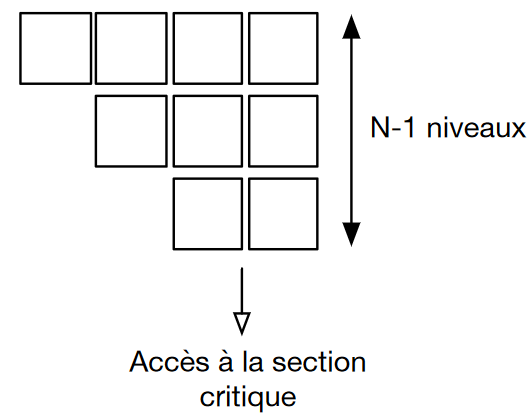
\includegraphics{image-25.png}
\caption{Alt text}
\end{figure}

Si des threads veulent passer il faut que: - Au moins 1 passe - Au moins
1 reste

Quand on est au dernier niveau avec 2 threads, un des deux passe et
l'autre attend.

Pour mettre cela en oeuvre, un thread qui annonce qu'il rentre dans un
nouveau niveau va laisser passer les autres d'abord.

On a 2 tableaux partagés. 1. \texttt{level{[}N{]}}: indexé par le
\textbf{numéro de Thread} et indique son niveau 2.
\texttt{victim{[}N{]}}: indexé par le \textbf{niveau} et dit quel thread
est en attente.

\begin{Shaded}
\begin{Highlighting}[]
\CommentTok{// Thread i}
\CommentTok{// Parcours des niveaux 1 à n{-}1}
\ControlFlowTok{for} \OperatorTok{(}\DataTypeTok{int}\NormalTok{ L }\OperatorTok{=} \DecValTok{1}\OperatorTok{;}\NormalTok{ L }\OperatorTok{\textless{}}\NormalTok{ N}\OperatorTok{;}\NormalTok{ L}\OperatorTok{++)} \OperatorTok{\{}
    \CommentTok{// Annoncer l\textquotesingle{}intention de rentrer au niveau L}
\NormalTok{    level}\OperatorTok{[}\NormalTok{i}\OperatorTok{]} \OperatorTok{=}\NormalTok{ L}\OperatorTok{;}
    \CommentTok{// Le thread se désigne comme la victime pour ce niveau}
\NormalTok{    victim}\OperatorTok{[}\NormalTok{L}\OperatorTok{]} \OperatorTok{=}\NormalTok{ i}\OperatorTok{;}
    \CommentTok{// Attendre tant qu\textquotesingle{}il existe au moins un thread au même niveau ou à un}
\NormalTok{    niveau supérieur}\OperatorTok{,}
    \CommentTok{// et que le thread i est la victime du niveau où il se trouve}
    \DataTypeTok{int}\NormalTok{ t\_niv\_sup\_egal }\OperatorTok{=} \DecValTok{0}\OperatorTok{;}
    \ControlFlowTok{do} \OperatorTok{\{}
    \ControlFlowTok{for} \OperatorTok{(}\DataTypeTok{int}\NormalTok{ j}\OperatorTok{=}\DecValTok{0}\OperatorTok{;}\NormalTok{ j}\OperatorTok{\textless{}}\NormalTok{ N}\OperatorTok{;}\NormalTok{ j}\OperatorTok{++)} \OperatorTok{\{}
        \CommentTok{// parcours du tableau des niveaux pour déterminer si un thread}
        \CommentTok{// est au même niveau ou à un niveau supérieur}
        \ControlFlowTok{if} \OperatorTok{((}\NormalTok{j}\OperatorTok{!=}\NormalTok{i}\OperatorTok{)} \OperatorTok{\&\&}\NormalTok{ level}\OperatorTok{[}\NormalTok{j}\OperatorTok{]} \OperatorTok{\textgreater{}=}\NormalTok{L}\OperatorTok{)} \OperatorTok{\{}
\NormalTok{            t\_niv\_sup\_egal }\OperatorTok{=} \DecValTok{1}\OperatorTok{;}
        \OperatorTok{\}}
    \OperatorTok{\}}
    \OperatorTok{\}} \ControlFlowTok{while} \OperatorTok{(}\NormalTok{t\_niv\_sup\_egal }\OperatorTok{\&\&}\NormalTok{ victim}\OperatorTok{[}\NormalTok{L}\OperatorTok{]==}\NormalTok{i}\OperatorTok{);}
\OperatorTok{\}}
\NormalTok{section\_critique}\OperatorTok{();}
\CommentTok{// Libération de threads bloqués en attente dans les niveaux inférieurs}
\NormalTok{level}\OperatorTok{[}\NormalTok{i}\OperatorTok{]=}\DecValTok{0}\OperatorTok{;}
\end{Highlighting}
\end{Shaded}

Si on décompose le code, on voit qu'un thread progresse si: - Il n'y
aucun thread en attente à son niveau - Il y a un autre thread qui a pris
le rôle de victime.

Au plus N-L threads peuvent dépasser le niveau L. Donc au plus 1 seul
thread peut accéder au niveau N-1.

\begin{figure}
\centering
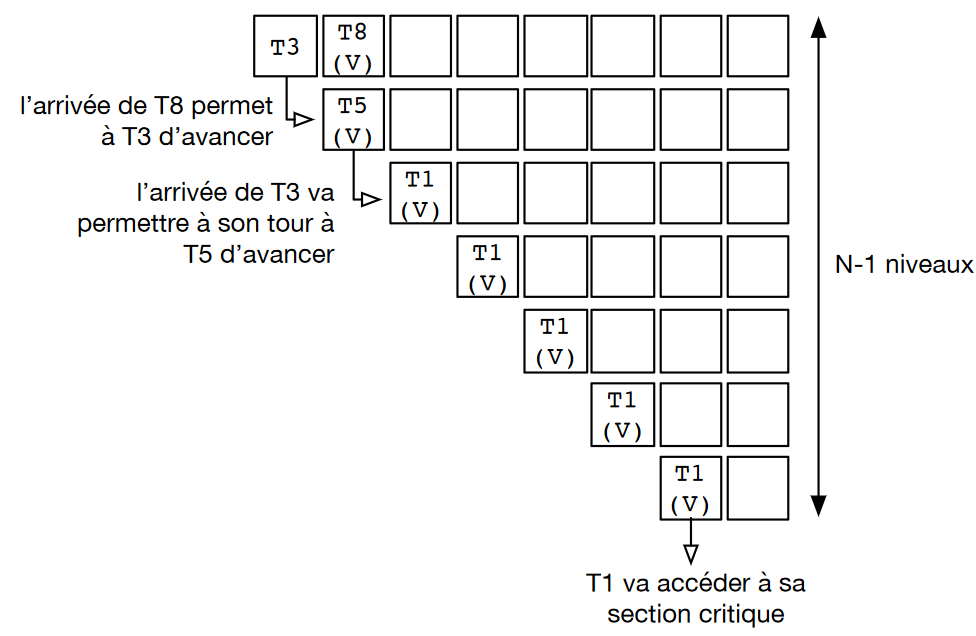
\includegraphics{image-26.png}
\caption{Alt text}
\end{figure}

\subsubsection{Équité}\label{uxe9quituxe9}

On n'a pas la garantie qu'un thread arrivé en premier tout au-dessus des
niveaux va s'exécuter que ceux arriver ! Cela dépend du temps alloué par
le processeur et ce cas de figure ci peut se passer:

\begin{figure}
\centering
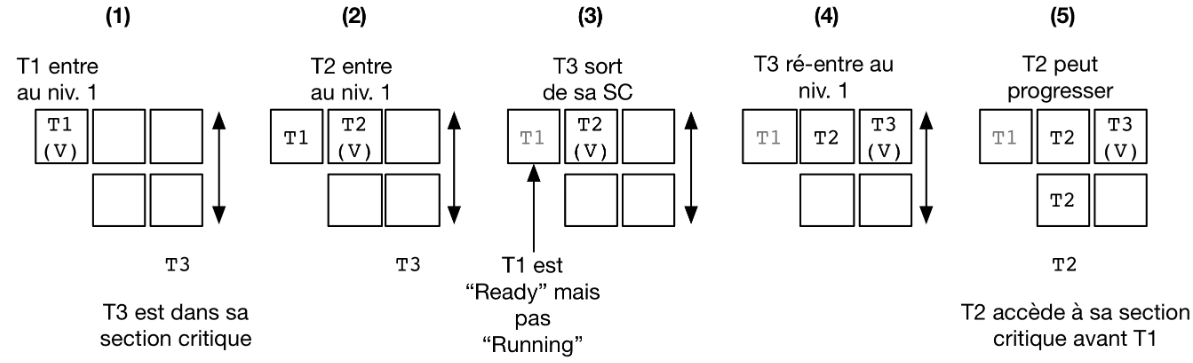
\includegraphics{image-27.png}
\caption{Alt text}
\end{figure}

Ceci arrive à partir de 3 threads.

On peut donc définir l'équité et rendre l'algorithme plus équitable
(permettant d'assurer la propriété de \textbf{liveness}). On va
subdiviser en 2 la partie d'accès à la section critique: 1.
\emph{Doorway}: en un nombre de pas borné, configuration de variables
partagées 2. \emph{Waiting}: boucle \texttt{while()} qui vérifie une
condition.

Garantie formelle d'équité : si la section doorway \(D_A\) d'un thread
\(T_A\) termine avant le début de la section doorway \(D_B\) d'un thread
\(T_B\), alors \(T_A\) a la garantie d'accéder à sa section critique
avant \(T_B\).

À savoir qu'on peut avoir une exécution concurrente de \(D_A\) et
\(D_B\) et donc l'ordre peut être arbitraire. On peut aussi avoir le
\emph{k-bounded waiting} donc pas plus de k sections critiques de
différences entre deux threads. FIFO c'est un 1-bounded waiting.

\subsection{Bakery Algorithm}\label{bakery-algorithm}

Se base sur les tickets de boucherie. On doit toujours savoir combien de
threads on a à l'avance. On a également 2 tableaux partagées: 1.
\texttt{drapeau{[}N{]}}: indexé par le \textbf{numéro du Thread} et
indique s'il veut rentrer en SC. 2. \texttt{ticket{[}N{]}}: indexé par
le \textbf{numéro du Thread} et indique le numéro dans la file.

\textbf{HYPOTHÈSES:} On a également des sections \textbf{doorway} qui ne
sont jamais concurrentes. On aura jamais 2 threads avec le même numéro
de ticket.

C'est \textbf{complètement} irréaliste de penser cela !! Par exemple, 2
threads peuvent observer le même état et donc prendre le même numéro de
ticket !

Donc on doit juste définir un \textbf{ordre de passage} pour les threads
ayant le même numéro ! Le plus simple est de prendre le thread avec le
plus petit numéro.

\begin{Shaded}
\begin{Highlighting}[]
\CommentTok{// Thread i}
\CommentTok{// Section doorway : annoncer son intérêt et obtenir un ticket}
\NormalTok{drapeau}\OperatorTok{[}\NormalTok{i}\OperatorTok{]=}\DecValTok{1}\OperatorTok{;}
\DataTypeTok{int}\NormalTok{ t}\OperatorTok{=}\DecValTok{0}\OperatorTok{;}
\CommentTok{// Parcours des tickets}
\ControlFlowTok{for} \OperatorTok{(}\DataTypeTok{int}\NormalTok{ j}\OperatorTok{=}\DecValTok{0}\OperatorTok{;}\NormalTok{ j}\OperatorTok{\textless{}}\NormalTok{N}\OperatorTok{;}\NormalTok{ j}\OperatorTok{++)} \OperatorTok{\{}
    \ControlFlowTok{if} \OperatorTok{(}\NormalTok{ticket}\OperatorTok{[}\NormalTok{j}\OperatorTok{]\textgreater{}}\NormalTok{t}\OperatorTok{)} \OperatorTok{\{}
\NormalTok{        t }\OperatorTok{=}\NormalTok{ ticket}\OperatorTok{[}\NormalTok{j}\OperatorTok{];}
    \OperatorTok{\}}
\OperatorTok{\}}

\CommentTok{// Prise du ticket supérieur}
\NormalTok{ticket}\OperatorTok{[}\NormalTok{i}\OperatorTok{]=}\NormalTok{t}\OperatorTok{+}\DecValTok{1}\OperatorTok{;}
\CommentTok{// Section waiting : attendre son tour ...}

\ControlFlowTok{do} \OperatorTok{\{}
    \DataTypeTok{int}\NormalTok{ mon\_tour }\OperatorTok{=} \DecValTok{1}\OperatorTok{;}
    \CommentTok{// Parcours des tickets des autres threads dont le drapeau est levé}
    \ControlFlowTok{for} \OperatorTok{(}\DataTypeTok{int}\NormalTok{ j}\OperatorTok{=}\DecValTok{0}\OperatorTok{;}\NormalTok{ j}\OperatorTok{\textless{}}\NormalTok{N}\OperatorTok{;}\NormalTok{ j}\OperatorTok{++)} \OperatorTok{\{}
        \ControlFlowTok{if} \OperatorTok{(}\NormalTok{drapeau}\OperatorTok{[}\NormalTok{j}\OperatorTok{])} \OperatorTok{\{}
            \ControlFlowTok{if} \OperatorTok{((}\NormalTok{ticket}\OperatorTok{[}\NormalTok{j}\OperatorTok{]} \OperatorTok{\textgreater{}}\NormalTok{ ticket}\OperatorTok{[}\NormalTok{i}\OperatorTok{])} \OperatorTok{||} \OperatorTok{((}\NormalTok{ticket}\OperatorTok{[}\NormalTok{j}\OperatorTok{]==}\NormalTok{ticket}\OperatorTok{[}\NormalTok{i}\OperatorTok{])} \OperatorTok{\&\&}\NormalTok{ j}\OperatorTok{\textgreater{}}\NormalTok{i}\OperatorTok{))} \OperatorTok{\{}
            \CommentTok{// Il y a un autre thread actif devant dans la file ...}
\NormalTok{                mon\_tour }\OperatorTok{=} \DecValTok{0}\OperatorTok{;}
            \OperatorTok{\}}
        \OperatorTok{\}}
    \OperatorTok{\}}
\OperatorTok{\}} \ControlFlowTok{while} \OperatorTok{(!}\NormalTok{mon\_tour}\OperatorTok{);}

\NormalTok{section\_critique}\OperatorTok{();}
\CommentTok{// Libération de threads en attente avec les tickets suivants}
\NormalTok{drapeau}\OperatorTok{[}\NormalTok{i}\OperatorTok{]=}\DecValTok{0}\OperatorTok{;}
\end{Highlighting}
\end{Shaded}

Ici, on utilise que des lecteurs écrivains pour mettre en place les
threads. On ne communique pas au \emph{scheduler} ce qui est mis en
pause. Ce n'est pas très optimal car on risque de donner de la ressource
à un thread qui ne peut progresser.

On pourrait faire des opérations sur le processeur pour palier à ça mais
ça ne va pas fonctionner ! En effet, l'ordinateur va ré-arranger les
instructions et les optimiser donc l'ordre d'exécution n'est pas
garanti.

Utiliser le mot-clé \texttt{volatile} pour forcer le programme à relire
tout le temps la valeur ne va pas non plus résoudre le problème à cause
des ordres d'exécution ``\emph{aléatoires}''. (Il existe des barrières
pour forcer des contraintes d'accès à la mémoire \texttt{MFENCE},
\texttt{LFENCE} et \texttt{SFENCE})

On va préférer utiliser des opérations atomiques

\section{Utilisation des Opérations
Atomiques}\label{utilisation-des-opuxe9rations-atomiques}

Une opération est: \emph{une opération qui ne peut être interrompue par
l'arrivée d'une interruption}. On réalise cela via un registre et un mot
mémoire. Les opérations sont donc exécutées de manière
\textbf{séquentielle}.

\subsection{\texorpdfstring{Instructions
\texttt{xchg}}{Instructions xchg}}\label{instructions-xchg}

\begin{Shaded}
\begin{Highlighting}[]
\NormalTok{xchgl \%eax, (var) }
\end{Highlighting}
\end{Shaded}

Équivalent:

\begin{Shaded}
\begin{Highlighting}[]
\NormalTok{movl (var), \%ebx}
\NormalTok{movl \%eax, (var)}
\NormalTok{movl \%ebx, \%eax}
\end{Highlighting}
\end{Shaded}

On a une exclusion mutuelle en utilisant simplement un unique mot
mémoire partagée (ils vont donc tenter d'écrire dans une variable lock 1
qui était libre 0).

\subsubsection{Exclusion Mutuelle}\label{exclusion-mutuelle}

Après un appel à un \texttt{xcgh} il y a deux possibilités: 1.
\texttt{\%eax} contient 0 : l'adresse (\texttt{lock}) a été mise de 0 à
1. * Donc est maintenant réservé et le thread peut rentrer en SC. 2.
\texttt{\%eax} contient 1 : l'adresse (\texttt{lock}) a été mise à 1
mais valait déjà 1 avant l'appel ! * Donc le \texttt{lock} n'était pas
libre ! On va donc boucler et ré-essayer

C'est une approche \emph{test-and-set}.

\subsubsection{Attente Active
(spinlocks)}\label{attente-active-spinlocks}

Les algorithmes basées sur une boucle \texttt{while} qui check une
condition à chaque fois sont appelés des algorithmes \emph{spinlocks}.

Cela fait du travail inutile pour le processeur. Vraiment problématique
pour du code sur mono-coeur car c'est inutile !

\subsubsection{Mutex POSIX}\label{mutex-posix}

On va ici utiliser le support du \textbf{Système d'Exploitation}. Si un
thread veut faire un \texttt{lock()} sur un mutex \emph{déjà bloqué}
alors ce thread sera mis en état \textbf{blocked}. Il est maintenant
dans une file d'attente pour que le mutex soit \texttt{unlock()}.

\textbf{Avantages:} On perd pas de ressources inutilement. Utile pour
gérer les sections critiques.

\textbf{Inconvénients:} On a une grande latence entre l'appel
\texttt{lock()} et l'exécution de la section critique.

\paragraph{Comparaison}\label{comparaison}

\textbf{Attente active} que sur multi-processeur. Utile pour les
sections critiques courtes. Fort utilisé dans le noyau !

\textbf{Mutex} plus efficace pour mettre en oeuvre la synchronisation
avec équité. On ne schedule pas des threads non prioritaires avant ceux
qui doivent accéder à leur SC en premier.

\subsection{\texorpdfstring{Test-and-set
\texttt{xchg}}{Test-and-set xchg}}\label{test-and-set-xchg}

Si on utilise cet algorithme avec un \texttt{xchg} c'est
\textbf{catastrophique}. On a une latence d'accès au sections critiques
qui augmentent avec le nombre de threads.

Ceci est causé par le \textbf{cache} !

\begin{figure}
\centering
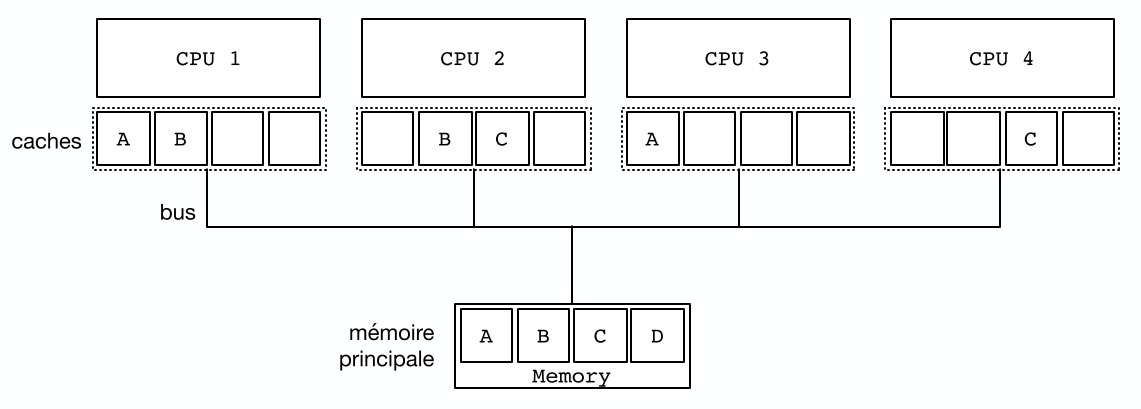
\includegraphics{image-28-1.png}
\caption{Alt text}
\end{figure}

On a donc un cache pour chaque coeur et les adresses mémoires récemment
utilisées. Mais on a aucun moyen de s'assurer de la cohérence du tout.

\subsubsection{Utilisation du Cache}\label{utilisation-du-cache}

On utilise donc le \emph{bus} pour coordonner la mise à jour et
l'invalidation de leur contenu.

On a chaque contrôleur qui \emph{snoop} le bus. Un seul contrôleur peut
utiliser le bus à un moment. La mémoire va donc écouter le bus et
répondre aux requêtes de lecture/écriture.

\subsubsection{Protocole de Cohérence de Cache
MSI}\label{protocole-de-cohuxe9rence-de-cache-msi}

Chaque ligne de cache a donc 3 états: - \textbf{M} \emph{modified}: la
valeur en cache est plus récente que celle en mémoire principale. -
\textbf{S} \emph{shared}: lignes présentes à d'autres endroits et
identiques. - \textbf{I} \emph{invalid}: on ne peut pas utiliser cette
ligne. L'accès doit retourner vers le bus pour avoir la version la plus
à jour.

\begin{figure}
\centering
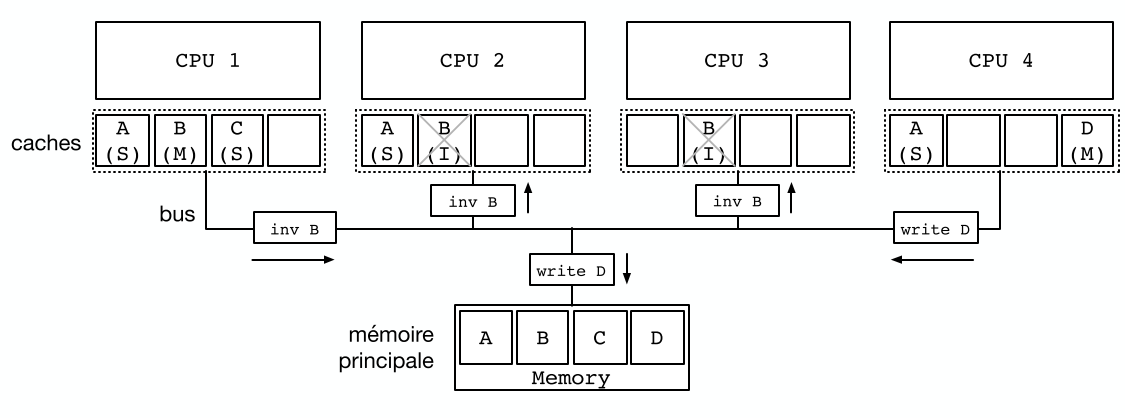
\includegraphics{image-29-1.png}
\caption{Fonctionnement MSI}
\end{figure}

Donc pour écrire une ligne en mode S, le contrôleur de cache doit
invalider les autres copies de S et passer la ligne en mode M.

Avec cela, on peut assister à un phénomène de ping-pong entre les caches
si deux threads s'exécutent sur des processeurs différents. À chaque
modification, un des deux threads doit invalider la valeur chez l'autre
et modifier le tout.

Le \textbf{faux partage} arrive lorsque deux variables distinctes sont
dans la même ligne de cache.

\subsubsection{Instructions Atomiques \& Utilisation du
Bus}\label{instructions-atomiques-utilisation-du-bus}

Avec un \texttt{xchg}, on doit avoir accès à la ligne de cache en mode
\textbf{M} mais aussi assurer qu'aucune opération concurrente ne soit
possible. Il faut verrouiller le bus le temps de l'exécution.

Donc il y a un coup pour le processeur qui l'exécute pour assurer
l'atomicité mais aussi pour les autres car ils ne peuvent plus rien
exécuter.

Donc on va saturer via un test-and-set le bus de message d'invalidation
et en le bloquant.

\paragraph{Solution:
test-and-test-and-set}\label{solution-test-and-test-and-set}

On tire profit que tant que la variable \texttt{lock} est à 1, le thread
\(T_A\) exécute sa section critique. On va éviter de faire des appels à
\texttt{xchg}. Tant que \texttt{lock} est à 1 on peut faire une lecture
depuis le cache et si on lit 0 alors il tente d'appeler \texttt{xchg}.

\begin{Shaded}
\begin{Highlighting}[]
\ControlFlowTok{while} \OperatorTok{(}\NormalTok{test\_and\_set}\OperatorTok{(}\NormalTok{verrou}\OperatorTok{,} \DecValTok{1}\OperatorTok{))} \OperatorTok{\{} 
    \CommentTok{// on a pas obtenu le verrou car on a lu 1 }
    \CommentTok{// donc on attend de lire 0 pour tenter à nouveau while (verrou) \{\}}
\OperatorTok{\}}
\end{Highlighting}
\end{Shaded}

\begin{figure}
\centering
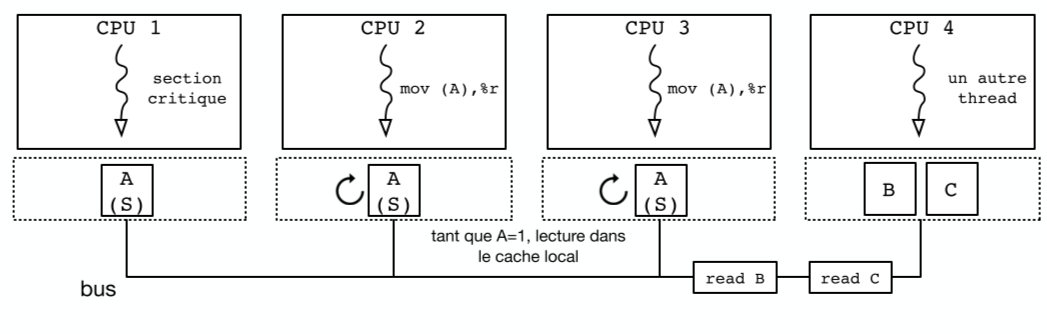
\includegraphics{image-30-1.png}
\caption{Alt text}
\end{figure}

Cela va réduire sensiblement le traffic et l'immobilisation du bus quand
la contention est élevée. Mais cela impact toujours de manière non
négligeable.

Dès que \texttt{lock} est libéré tous les autres threads se jettent pour
appeler \texttt{xchg}. Des essais infructueux a de lourds impacts sur le
système. Cela augmente la contention.

\paragraph{backoff-test-and-test-and-test}\label{backoff-test-and-test-and-test}

On peut aussi attendre et revenir plus tard !

Si lors d'un second essai la contention est toujours forte on va
attendre encore plus longtemps. On adapte les ressources nécessaires en
fonction du trafic.

On va souvent utiliser du \textbf{exponentiel-backoff}. Si on arrive pas
du premier coup, on va attendre un temps aléatoire entre
\texttt{{[}0:v{]}} avec \(v=v_{init}\). Au deuxième essai, on attendra
\(v=v*2\) et cela jusqu'à \(v_{max}\) et on ne doit pas utiliser d'appel
système pour l'attente.

\subsection{Conclusion}\label{conclusion}

\begin{itemize}
\tightlist
\item
  Le problème fondamental à résoudre pour construire des primitives de
  synchronisation est celui de l'exclusion mutuelle

  \begin{itemize}
  \tightlist
  \item
    Avec des garanties de liveness : pas de \emph{livelock} ou
    d'hypothèses sur l'entrelacement des opérations
  \end{itemize}
\item
  Algorithmes classiques difficiles à utiliser sur les architectures
  modernes car fondés sur des hypothèses sur l'ordre des accès mémoire
  et une utilisation de la mémoire en \(O(N)\)
\item
  Utilisation d'instructions atomiques pour résoudre l'exclusion
  mutuelle avec \(O(1)\) mot partagé
\item
  Attention à la mise en oeuvre et à l'impact sur le cache et la
  performance !
\end{itemize}

\section{Scheduling}\label{scheduling}

\subsection{Rappel}\label{rappel}

Les SE tel que Linux supporte d'avoir un grand nombre de thread (parfois
sur des mono-processeurs). On doit donc partager. On crée l'illusion de
continuité.

\subsection{Mécanisme \& Politique}\label{muxe9canisme-politique}

\begin{itemize}
\tightlist
\item
  \textbf{Mécanisme:} (\emph{ex:} changement de contexte (sauvegarde et
  restauration)) cela permet d'\textbf{acter des décisions de placement
  de threads sur les processus}.
\item
  \textbf{Politique} (\emph{ex:} scheduler ) cela permet de
  \textbf{prendre des des décisions de placement} (ou va chaque
  threads).
\end{itemize}

Donc on peut avoir plusieurs politiques possibles sur la base du même
mécanisme.

\subsubsection{Exécution des Threads}\label{exuxe9cution-des-threads}

\begin{figure}
\centering
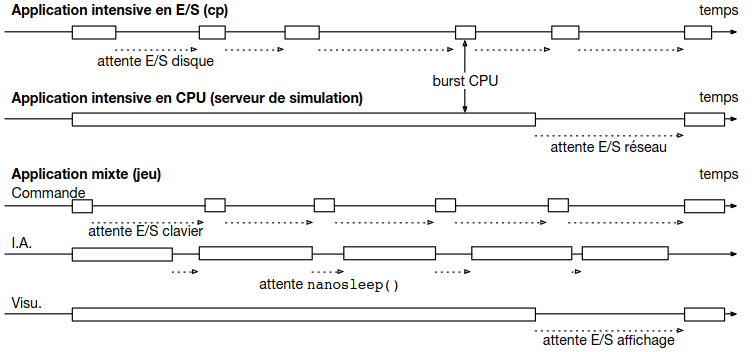
\includegraphics{image-28.png}
\caption{Alt text}
\end{figure}

On a une alternance entre:

\begin{enumerate}
\def\labelenumi{\arabic{enumi}.}
\tightlist
\item
  \textbf{Burst CPU}
\item
  \textbf{Opération bloquante}
\end{enumerate}

Sur le schéma ci-dessus, on voit la durée de différent burst CPU et les
moments d'attente.

\begin{figure}
\centering
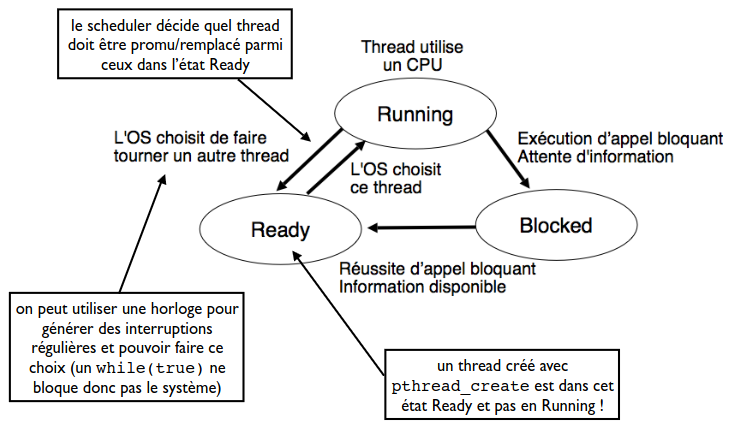
\includegraphics{image-29.png}
\caption{une image vaut mieux que mille mots}
\end{figure}

\subsubsection{Évolution de l'État d'un
Thread}\label{uxe9volution-de-luxe9tat-dun-thread}

\paragraph{\texorpdfstring{Passage de \emph{Running} à
\emph{Blocked}}{Passage de Running à Blocked}}\label{passage-de-running-uxe0-blocked}

\begin{itemize}
\tightlist
\item
  Appel système \emph{bloquant} (ex: \emph{pthread\_mutex\_lock(3
  posix)}, \emph{read(2)}, \emph{sem\_wait(3posix)})
\end{itemize}

Les threads en état Blocked associés à une structure de donnée jouant le
rôle d'une \emph{salle d'attente}.

\begin{itemize}
\tightlist
\item
  \emph{Thread Unique}: attente de la fin d'une entrée/sortie demandée
  par ce thread
\item
  \emph{Plusieurs Threads}: attente sur une ressource partagée (type
  \emph{sémaphore} / \emph{mutex})
\end{itemize}

\begin{figure}
\centering
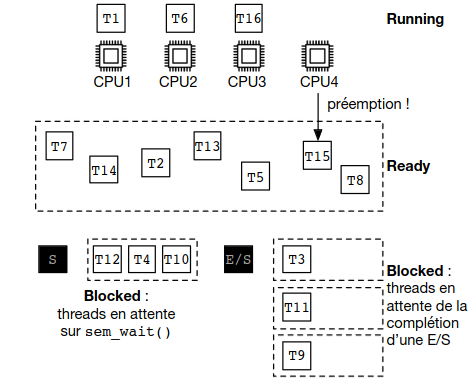
\includegraphics{image-30.png}
\caption{Alt text}
\end{figure}

On a aucune garantie sur l'ordre de réveil de thread

\paragraph{\texorpdfstring{Passage de \emph{Running} à
\emph{Ready}}{Passage de Running à Ready}}\label{passage-de-running-uxe0-ready}

On va sé prémunir des programmes qui sont \emph{infiniment} en mode
\emph{ready}.

Le SE va faire des interruptions périodiques générées par une horloge.
Ensuite, le SE peut décider de \textbf{ne pas restaurer} le thread
Running. On appelle cela la \textbf{préemption}.

\paragraph{\texorpdfstring{Passage de \emph{Ready} à
\emph{Running}}{Passage de Ready à Running}}\label{passage-de-ready-uxe0-running}

Le \emph{Scheduler} a décidé de restaurer l'état de ce thread sur le
processeur.

\subsection{Scheduler}\label{scheduler}

Le \emph{Scheduler} fait une \textbf{politique d'ordonnancement}. Ce
dernier prend des décisions à deux occasions:

\begin{enumerate}
\def\labelenumi{\arabic{enumi}.}
\tightlist
\item
  \textbf{Processeur disponible}: à la fin d'un CPU Burst.
\item
  \textbf{Interruption périodique}: peut arriver pendant un CPU Burst.
\end{enumerate}

Dans le cas 2. le scheduler est donc \textbf{préemptif}.

\paragraph{Scheduler Universel}\label{scheduler-universel}

Il n'y a pas de scheduler parfait.

\subsubsection{Objectifs}\label{objectifs}

On doit faire un compromis entre différents objectifs:

\begin{itemize}
\tightlist
\item
  \textbf{Objectifs Systèmes:}

  \begin{itemize}
  \tightlist
  \item
    Maximiser l'utilisation processeur
  \item
    Maximiser le débit applicatif
  \end{itemize}
\item
  \textbf{Objectifs pour chaque Application:}

  \begin{itemize}
  \tightlist
  \item
    Minimiser le temps d'exécution total (pas de sens pour application
    interactive)
  \item
    Minimiser le temps d'attente (entre \emph{Ready} vers
    \emph{Running})
  \item
    Minimiser le temps de réponse (entre \emph{Ready} vers
    \emph{Blocked})
  \item
    Équité des métriques
  \end{itemize}
\end{itemize}

\subsubsection{Scheduler FCFS}\label{scheduler-fcfs}

\textbf{First-Come First-Serve}. Le scheduler est donc non préemptif car
un thread Running complète tout son burst CPU.

Ainsi avec 4 threads avec un temps d'exécution respectif de 5,4,2 et 7
secondes. On peut avoir une attente moyenne de 7 ou 5 secondes.

Ce n'est pas optimal pour des burst CPU plus court qui sont coincés
derrière des burst plus long.

\subsubsection{Scheduler SJF}\label{scheduler-sjf}

Choisit le thread Ready avec le burst CPU le plus court. Toujours non
préemptif. Et va trouver le temps le plus court (dans notre exemple
d'au-dessus, le temps d'attente moyen le plus court est 4.25 secondes).

Mais connaître le temps d'arrêt d'un thread revient à transgresser le
\textbf{problème de l'arrêt}.

On peut néanmoins prédire les prochains burst basés sur les précédents.
On va donc utiliser des moyennes pondérées comme estimation.

\begin{figure}
\centering
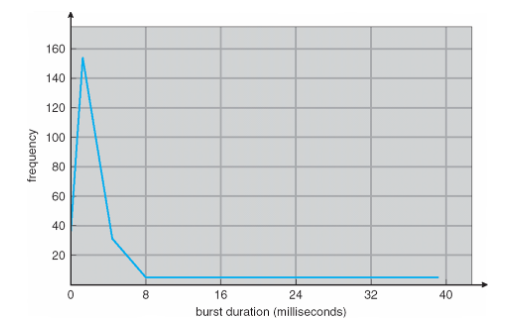
\includegraphics{image-31.png}
\caption{Burst typique}
\end{figure}

Avec ce type d'organisation, les bursts les plus longs risquent de
rester bloquer derrière les plus courts de manière indéfinie.

\subsubsection{Scheduler Préemptif RR}\label{scheduler-pruxe9emptif-rr}

On peut libérer le processeur à chaque tick de l'horloge système. C'est
un équivalent de \emph{Round-Robin} (ruban rond).

\begin{figure}
\centering
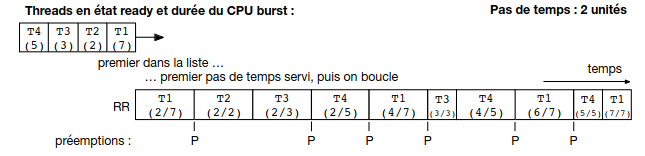
\includegraphics{image-32.png}
\caption{Alt text}
\end{figure}

\begin{itemize}
\tightlist
\item
  ✅ Ainsi, on a un temps d'attente moyen assez court.
\item
  ❌ Pas de relation directe entre \emph{attente} et \emph{temps de
  réponse}
\item
  ❌ Beaucoup de changement de contexte
\item
  ❌ Pas de distinction entre threads avec bursts courts et longs
\end{itemize}

\paragraph{Fréquence d'horloge}\label{fruxe9quence-dhorloge}

Au + la fréquence est haute, au - temps d'attente des threads
\textbf{mais} + de consommation d'énergie et - d'utilisation utile du
CPU

\begin{itemize}
\tightlist
\item
  1990: 100 Hz
\item
  2000: 1 kHz
\item
  2010+: fréquence adaptive (base clock et boost clock). Pas de réveil
  d'un processeur en veille si pas de thread \emph{Ready}. Pas
  d'interruption si un seul thread \emph{Running} et pas de
  \emph{Ready}.
\end{itemize}

\subsubsection{Scheduler à Priorité}\label{scheduler-uxe0-priorituxe9}

Pas la même priorité pour différentes applications: \emph{daemon} vs
\emph{application utilisée par l'utilisateur à l'instant t}.

Pareil pour les threads, certains vont demander de la réactivité et des
ressources et d'autres non.

On va exécuter le thread avec la plus haute priorité d'abord. On
maintient une liste circulaire. Il faut faire attention au problème de
famine

\paragraph{Problème de Famine}\label{probluxe8me-de-famine}

On utilise des priorités adaptatives (\emph{basse} et \emph{courante}).

Au départ: priorité courante = priorité de base

À chaque exécution d'un burst CPU, la priorité courante diminue. On
réalise un nouveau cycle quand tous les threads ont une priorité
courante = 0.

\paragraph{Tout Combiner}\label{tout-combiner}

On combine les principes de priorité + préemption.

\begin{itemize}
\tightlist
\item
  Thread passe Running: on lui alloue un temps d'exécution maximale =
  \textbf{quantum} (longueur du quantum = multiple de la période de
  l'horloge système).
\item
  Thread termine dans les temps sinon préemption.
\item
  Utilisation de priorités fixes et courantes (courante diminue à chaque
  burst CPU).
\end{itemize}

\begin{figure}
\centering
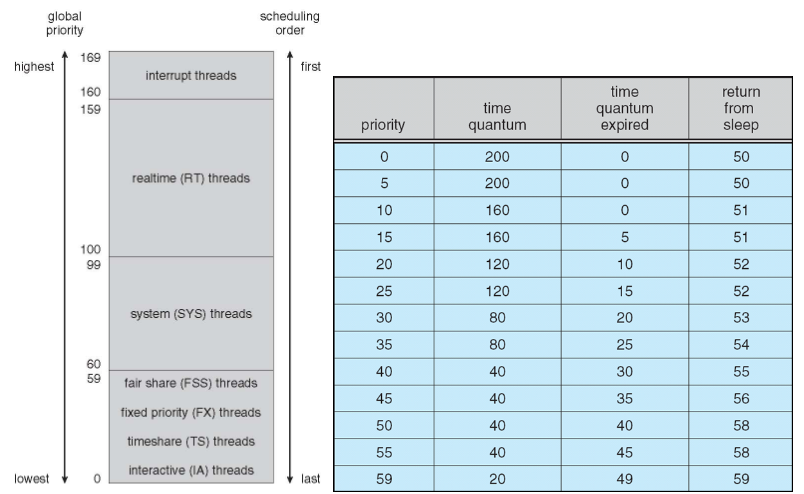
\includegraphics{image-33.png}
\caption{Alt text}
\end{figure}

\paragraph{Synchronisation des
Threads}\label{synchronisation-des-threads}

Il vaut mieux laisser un thread de priorité basse finir sa section
critique plutôt que de la préempter.

\begin{itemize}
\tightlist
\item
  \textbf{\emph{Priority ceiling:}}
  \texttt{pthread\_mutexattr\_setprioceiling()}

  \begin{itemize}
  \tightlist
  \item
    Associe un mutex de priorité donné au thread le temps de sa SC. Fixé
    au max des priorités des threads accédant au mutex.
  \item
    Évite la préemption par le thread de priorité plus élevée. Risque
    d'interférence avec les autres threads haute priorité dy système car
    fait systématiquement.
  \end{itemize}
\item
  \textbf{\emph{Priority inheritance:}}

  \begin{itemize}
  \tightlist
  \item
    La priorité du thread avec un mutex est fixée au max de celle des
    threads en attente sur ce mutex.
  \item
    N'évite pas la première préemption mais booste la priorité d'un
    thread de priorité faible dans le cas général.
  \end{itemize}
\end{itemize}

\paragraph{Priorité des Processus}\label{priorituxe9-des-processus}

Par défaut, les threads d'un processus héritent de la priorité du
premier thread du processus. Dépend donc de l'environnement d'exécution.

Si on est pas \texttt{root}, on ne peut pas demander des priorités plus
élevés mais \emph{seulement} plus faibles.

On fait cela via l'utilitaire \texttt{nice(1)} ou la fonction
\texttt{nice(2)}.

\begin{itemize}
\tightlist
\item
  \(>0\): priorité plus faible (jusqu'à 20)
\item
  \(<0\); priorité plus élevé (jusqu'à -19)
\end{itemize}

\subsection{Conclusion}\label{conclusion}

À la base d'un même mécanisme de changement de contexte, plusieurs
politiques différentes possibles

\begin{itemize}
\tightlist
\item
  On peut utiliser de l'apprentissage automatique pour améliorer les
  paramètre d'un scheduler
\end{itemize}

Dans Linux, les priorités sont dynamiques et prise en compte des threads
\emph{interactifs}/\emph{intensifs} en CPU.

\begin{itemize}
\tightlist
\item
  Le noyau supporte de nombreux scheduler différents
\item
  Chaque scheduler peut être paramétré
\item
  Critique pour la bonne performance et l'efficacité énergétique
\end{itemize}

\section{Cours 10}\label{cours-10}

\subsection{La mémoire}\label{la-muxe9moire}

\href{../README.md}{\textless--}

\begin{center}\rule{0.5\linewidth}{0.5pt}\end{center}

\section{Gestion des utilisateurs}\label{gestion-des-utilisateurs}

Unix est pensé pour supporter plusieurs utilisateurs. On doit d'abord
s'authentifier

\subsection{Authentification}\label{authentification}

On se connecte via un mot de passe en local ou distant (\emph{ssh}). Il
existe aussi les authentifications par données biométriques,
cryptographie asymétrique (private key and public key).

Le premier processus au démarrage est le processus de \texttt{login} qui
va lui fork tous les autres sous-processus. On liste tous les users dans
\texttt{/etc/passwd}. On y stockait avant les mots de passe dedans mais
maintenant on les stocke dans des fichiers séparés (\emph{shadow
password}).

\subsubsection{\texorpdfstring{\texttt{/etc/passwd}}{/etc/passwd}}\label{etcpasswd}

\texttt{oracle:x:1021:1020:Oracle\ user:/data/network/oracle:/bin/bash}

\texttt{1:2:3:4:5:6:7}

\begin{enumerate}
\def\labelenumi{\arabic{enumi}.}
\tightlist
\item
  Nom d'utilisateur
\item
  Mot de passe (stocké dans \texttt{/etc/shadow})
\item
  Identifiant User (\textbf{UID})
\item
  Identifiant du groupe \emph{principal} de l'user (\textbf{GID})
\item
  Informations supplémentaires, nom complet de l'user
\item
  Répertoire \emph{home}
\item
  Shell à exécuter au moment du login de l'user
\end{enumerate}

\subsubsection{Types d'user}\label{types-duser}

\begin{longtable}[]{@{}
  >{\centering\arraybackslash}p{(\columnwidth - 2\tabcolsep) * \real{0.1081}}
  >{\centering\arraybackslash}p{(\columnwidth - 2\tabcolsep) * \real{0.8919}}@{}}
\toprule\noalign{}
\begin{minipage}[b]{\linewidth}\centering
type d'user
\end{minipage} & \begin{minipage}[b]{\linewidth}\centering
Description
\end{minipage} \\
\midrule\noalign{}
\endhead
\bottomrule\noalign{}
\endlastfoot
root & Aucune restriction et peut tout faire. Admin du système. \\
User normal & Droit limité mais peut obtenir des droits de root via
\texttt{sudo}. \\
User système & Ne correspond pas un réel user mais correspond à des
services du SE. (typiquement des daemons, \ldots) \\
\end{longtable}

\paragraph{\texorpdfstring{Obtenir leur
\textbf{UID}}{Obtenir leur UID}}\label{obtenir-leur-uid}

On utilise la fonction \texttt{getuid(2)} pour obtenir l'\textbf{UID} et
\texttt{geteuid(2)} pour obtenir l'\emph{effective \textbf{UID}} car il
se peut que les droits changent temporairement (\texttt{sudo}).

\paragraph{\texorpdfstring{Changer
l'\textbf{UID}}{Changer l'UID}}\label{changer-luid}

On peut faire cela via \texttt{setuid(2)} qui modifie l'UID de
l'utilisateur en cours d'exécution. Donc Root appelle \texttt{setuid}
avant \texttt{execve} pour se donner les droits d'administration.

\section{Systèmes de fichiers}\label{systuxe8mes-de-fichiers}

Il y a énormément de diversité en terme de support de stockage de
données. Il faut donc une interface \emph{commune}. En \textbf{UNIX},
les fichiers sont regroupés sous forme d'une arborescence unique.

\subsection{Hiérarchie et Montage}\label{hiuxe9rarchie-et-montage}

\begin{figure}
\centering
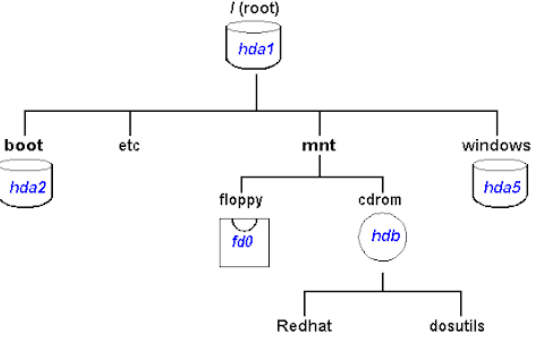
\includegraphics{image-34.png}
\caption{Alt text}
\end{figure}

En utilisant \texttt{mnt} on peut attacher ou détacher des systèmes de
fichiers dans la hiérarchie commune.

\subsection{contenu d'un répertoire}\label{contenu-dun-ruxe9pertoire}

\begin{verbatim}
$ ls -la / 
total 1488
drwxr-xr-x  19 root root    4096 Dec  9 14:35 .
drwxr-xr-x  19 root root    4096 Dec  9 14:35 ..
lrwxrwxrwx   1 root root       7 Apr 23  2020 bin -> usr/bin
drwxr-xr-x   2 root root    4096 Apr 23  2020 boot
drwxr-xr-x   9 root root    2820 Dec  9 14:35 dev
drwxr-xr-x 131 root root   12288 Dec  9 14:35 etc
drwxr-xr-x   3 root root    4096 Nov 15  2021 home
-rwxr-xr-x   3 root root 1440152 May  7  2022 init
lrwxrwxrwx   1 root root       7 Apr 23  2020 lib -> usr/lib
lrwxrwxrwx   1 root root       9 Apr 23  2020 lib32 -> usr/lib32
lrwxrwxrwx   1 root root       9 Apr 23  2020 lib64 -> usr/lib64
lrwxrwxrwx   1 root root      10 Apr 23  2020 libx32 -> usr/libx32
drwx------   2 root root   16384 Apr 10  2019 lost+found
drwxr-xr-x   2 root root    4096 Apr 23  2020 media
drwxr-xr-x   6 root root    4096 Sep 19 23:43 mnt
drwxr-xr-x   2 root root    4096 Apr 23  2020 opt
dr-xr-xr-x 244 root root       0 Dec  9 14:35 proc
drwx------   2 root root    4096 Feb 21  2023 root
drwxr-xr-x   6 root root     120 Dec  9 14:35 run
lrwxrwxrwx   1 root root       8 Apr 23  2020 sbin -> usr/sbin
drwxr-xr-x   2 root root    4096 Apr 10  2020 snap
drwxr-xr-x   2 root root    4096 Apr 23  2020 srv
dr-xr-xr-x  11 root root       0 Dec  9 14:35 sys
drwxrwxrwt  13 root root    4096 Dec  9 14:35 tmp
drwxr-xr-x  14 root root    4096 Apr 23  2020 usr
drwxr-xr-x  13 root root    4096 Apr 23  2020 var
\end{verbatim}

\subsubsection{Permissions}\label{permissions}

En analysant la première colonne, on peut savoir quelles sont les
permissions et si c'est un lien symbolique, hardlink ou directory.

On encode les permissions sur 9 bits via User (rwx), Groupe (rwx),
Autres (rwx). Ainsi, on connait les droits si on a le même UID, GUID ou
UID et GUID différents.

\begin{longtable}[]{@{}
  >{\centering\arraybackslash}p{(\columnwidth - 2\tabcolsep) * \real{0.0388}}
  >{\centering\arraybackslash}p{(\columnwidth - 2\tabcolsep) * \real{0.9612}}@{}}
\toprule\noalign{}
\begin{minipage}[b]{\linewidth}\centering
Droit
\end{minipage} & \begin{minipage}[b]{\linewidth}\centering
Description
\end{minipage} \\
\midrule\noalign{}
\endhead
\bottomrule\noalign{}
\endlastfoot
\texttt{r} & \emph{read}: lire le fichier, lister le contenu du
répertoire \\
\texttt{w} & \emph{write}: écrire dans le fichier, créer une entrée dans
le répertoire \\
\texttt{x} & \emph{execute}: accepter pour faire \texttt{execve} pour un
fichier. Pour un répertoire, on peut accéder à un fichier ou
sous-répertoire \\
\end{longtable}

\paragraph{\texorpdfstring{Subtilité du
\texttt{x}}{Subtilité du x}}\label{subtilituxe9-du-x}

\begin{verbatim}
$ mkdir -p repertoire 
$ echo "LINFO1252" > repertoire/fichier 
$ chmod 000 repertoire/ 
$ ls -al repertoire/
ls: cannot open directory repertoire/: Permission denied 
$ cat repertoire/fichier
cat: repertoire/fichier: Permission denied 
$ chmod +x repertoire/ 
$ ls -al repertoire/
ls: cannot open directory repertoire/: Permission denied
$ cat repertoire/fichier
LINFO1252
\end{verbatim}

\texttt{chmod} va changer les droits. On ne peut plus lister le fichier
car on a pas \texttt{r} mais on peut quand même y accéder car on a
\texttt{x} pour aller dans d'autres sous fichiers.

On représente les permissions comme 3 séquences de 3 bits donc
\texttt{rwxr-xr-\/-} = \texttt{754}. En utilisant \texttt{S\_ISUID} pour
un exécutable, permet l'exécution avec les permissions du propriétaire
de l'exécutable et pas celles de l'utilisateur.

\subsubsection{Navigation}\label{navigation}

Pour changer de répertoire en C où on exécute, on peut réaliser l'appel
suivant:

\begin{Shaded}
\begin{Highlighting}[]
\PreprocessorTok{\#include }\ImportTok{\textless{}unistd.h\textgreater{}}\PreprocessorTok{ }
\DataTypeTok{int}\NormalTok{ chdir}\OperatorTok{(}\DataTypeTok{const} \DataTypeTok{char} \OperatorTok{*}\NormalTok{path}\OperatorTok{);}
\end{Highlighting}
\end{Shaded}

\subsubsection{Fonctions Utiles}\label{fonctions-utiles}

\begin{longtable}[]{@{}
  >{\centering\arraybackslash}p{(\columnwidth - 2\tabcolsep) * \real{0.3070}}
  >{\centering\arraybackslash}p{(\columnwidth - 2\tabcolsep) * \real{0.6930}}@{}}
\toprule\noalign{}
\begin{minipage}[b]{\linewidth}\centering
Fonction
\end{minipage} & \begin{minipage}[b]{\linewidth}\centering
description
\end{minipage} \\
\midrule\noalign{}
\endhead
\bottomrule\noalign{}
\endlastfoot
\texttt{stat} & récupère les méta-données associées à un fichier ou
répertoire \\
\texttt{chmod}/\texttt{chown} & modifier les permissions ou le
propriétaire/groupe \\
\texttt{utime} & modifier les dates de création/modifications d'un
fichier (e.g.~commande \texttt{touch}) \\
\texttt{rename} & changer de nom, d'emplacement \\
\texttt{mkdir}/\texttt{rmdir} & créer/détruire un répertoire \\
\texttt{opendir}/\texttt{closedir}/\texttt{readir} & consulter le
contenu des répertoires \\
\end{longtable}

\subsubsection{Parcours de répertoire}\label{parcours-de-ruxe9pertoire}

\begin{Shaded}
\begin{Highlighting}[]
\KeywordTok{struct}\NormalTok{ dirent }\OperatorTok{\{} 
\NormalTok{    ino\_t d\_ino}\OperatorTok{;}                \CommentTok{/* inode number */}
\NormalTok{    off\_t d\_off}\OperatorTok{;}                \CommentTok{/* offset to the next dirent */} 
    \DataTypeTok{unsigned} \DataTypeTok{short}\NormalTok{ d\_reclen}\OperatorTok{;}    \CommentTok{/* length of this record */}
    \DataTypeTok{unsigned} \DataTypeTok{char}\NormalTok{ d\_type}\OperatorTok{;}       \CommentTok{/* type of file; not supported by all file system types */}
    \DataTypeTok{char}\NormalTok{ d\_name}\OperatorTok{[}\DecValTok{256}\OperatorTok{];}           \CommentTok{/* filename */}
\OperatorTok{\};}
\end{Highlighting}
\end{Shaded}

Il faut d'abord avoir ouvert un répertoire via \texttt{opendir}.
\texttt{readdir} pour accéder aux entrées du système.

TODO le reste

\begin{center}\rule{0.5\linewidth}{0.5pt}\end{center}

\href{../README.md}{\textless--}

\href{../README.md}{\textless--}

\begin{center}\rule{0.5\linewidth}{0.5pt}\end{center}

\section{Cours 12}\label{cours-12}

\begin{itemize}
\tightlist
\item
  \hyperref[cours-12]{Cours 12}

  \begin{itemize}
  \tightlist
  \item
    \hyperref[rappels]{Rappels}
  \item
    \hyperref[abstraction-du-matuxe9riel]{Abstraction du Matériel}

    \begin{itemize}
    \tightlist
    \item
      \hyperref[les-partitions]{Les partitions}
    \end{itemize}
  \end{itemize}
\item
  \hyperref[structure-dun-systuxe8me-de-fichier]{Structure d'un Système
  de Fichier}

  \begin{itemize}
  \tightlist
  \item
    \hyperref[stockage-et-allocation-des-blocs]{Stockage et Allocation
    des Blocs}

    \begin{itemize}
    \tightlist
    \item
      \hyperref[option-1]{Option 1}
    \item
      \hyperref[option-2]{Option 2}
    \item
      \hyperref[fat32]{FAT32}
    \item
      \hyperref[stockage-indexuxe9]{Stockage indexé}
    \item
      \hyperref[systuxe8me-de-fichiers-ext4]{Système de Fichiers
      \texttt{ext4}}
    \end{itemize}
  \item
    \hyperref[stockage-des-ruxe9pertoires]{Stockage des Répertoires}
  \item
    \hyperref[gestion-de-lespace-libre]{Gestion de l'Espace Libre}

    \begin{itemize}
    \tightlist
    \item
      \hyperref[effacer-un-fichier]{Effacer un Fichier}
    \item
      \hyperref[performance-et-cache]{Performance et Cache}
    \end{itemize}
  \item
    \hyperref[optimisations]{Optimisations}

    \begin{itemize}
    \tightlist
    \item
      \hyperref[robustesse]{Robustesse}
    \end{itemize}
  \end{itemize}
\end{itemize}

\subsection{Rappels}\label{rappels}

Le \emph{système de fichier} est une interface \emph{unifiée} et unique
des différents périphériques de stockage (car bcp de type différent). On
a une hiérarchie en \textbf{point de montage} (\texttt{mnt})

On a une grande diversité des supports: 1. Les Disques Durs avec des
têtes de lectures basé sur les champs électro-magnétique

\begin{figure}
\centering
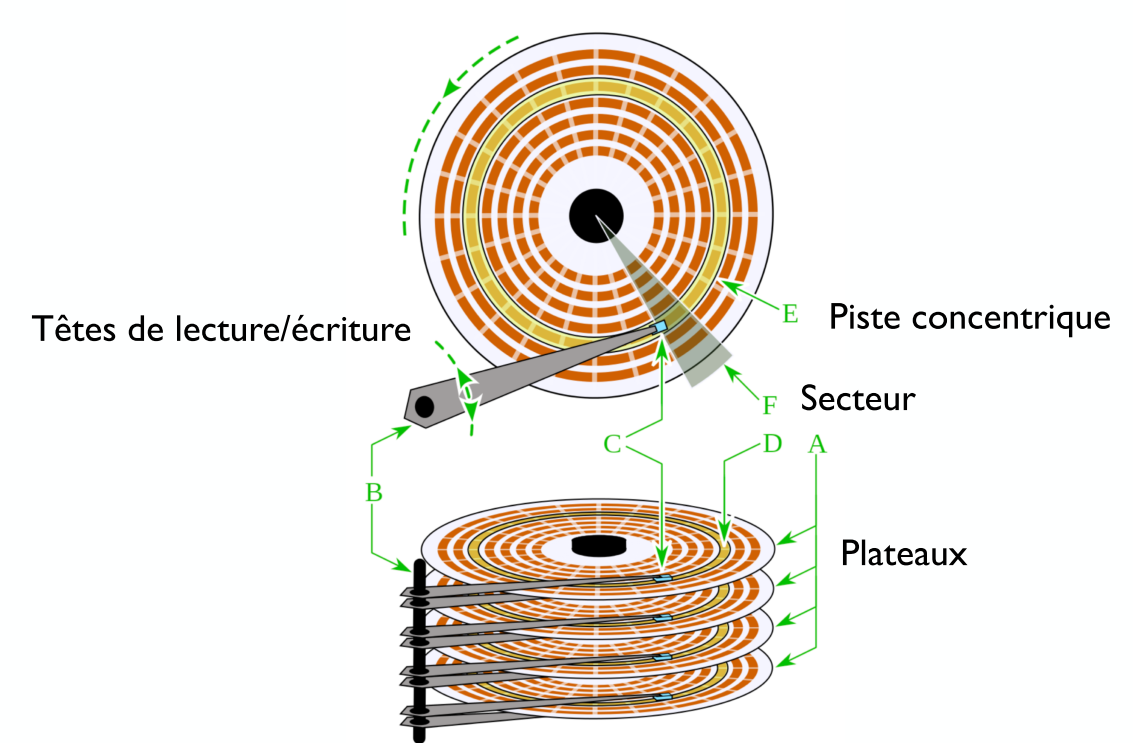
\includegraphics{image-35.png}
\caption{Alt text}
\end{figure}

\begin{enumerate}
\def\labelenumi{\arabic{enumi}.}
\setcounter{enumi}{1}
\tightlist
\item
  SSD: plus compliqué avec du flash, de la RAM buffer, \ldots{}
\end{enumerate}

\begin{figure}
\centering
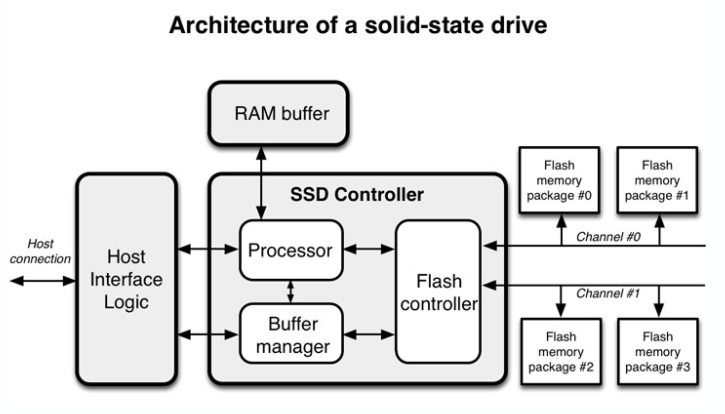
\includegraphics{image-36.png}
\caption{Alt text}
\end{figure}

\subsection{Abstraction du Matériel}\label{abstraction-du-matuxe9riel}

On a néanmoins une abstraction du matériel à faire pour que tout
fonctionne de manière uniforme:

\begin{figure}
\centering
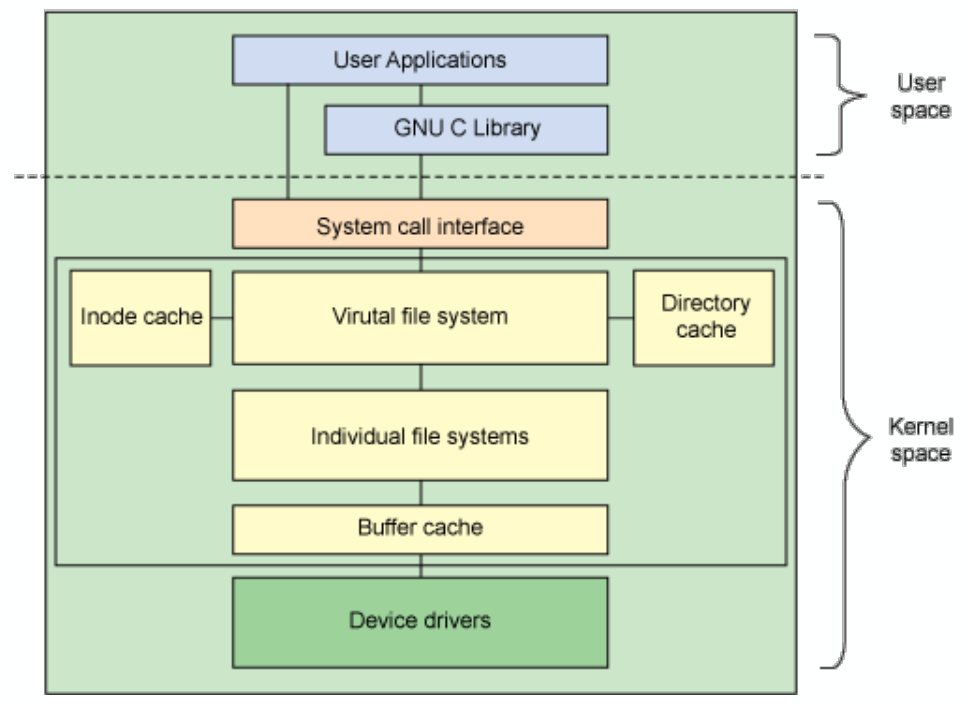
\includegraphics{image-37.png}
\caption{Alt text}
\end{figure}

Le fait qu'un dispositif de stockage utilise des plateaux, ram, \ldots{}
est géré via les \emph{devices drivers} et le \emph{gestionnaire de
périphérique} (interface logiciel kernel/matériel).

Comme précédemment, on va gérer le stockage via des blocs de
\texttt{4\ Ko} (même taille qu'un page mémoire wow). On peut tout de
même avoir une \textbf{granularité} différente (typiquement:
\texttt{512} octets pour un HDD et entre \texttt{256} et \texttt{4096}
octets pour un SSD).

\subsubsection{Les partitions}\label{les-partitions}

C'est le faite de virtuellement segmenter un support de stockage en
multiples morceaux.

On va retrouver au début des disques des
\textbf{\texttt{boot\ control\ block}} et dans chaque début de
\textbf{partitions} des \textbf{\texttt{partition\ control\ block}}.

\begin{figure}
\centering
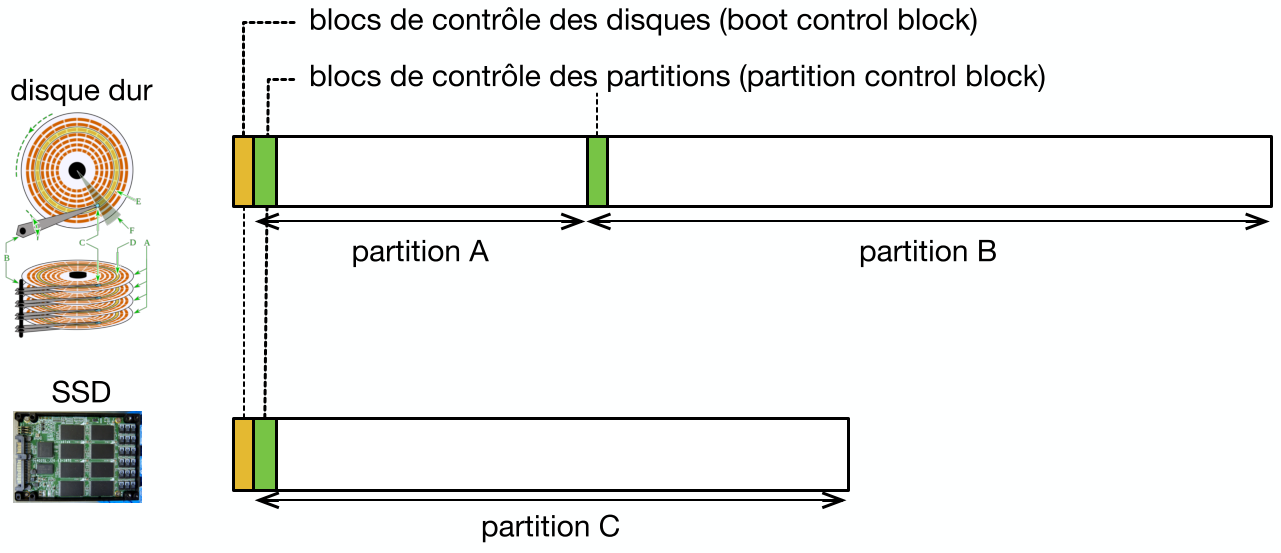
\includegraphics{image-39.png}
\caption{Alt text}
\end{figure}

\paragraph{\texorpdfstring{\texttt{boot\ control\ block}}{boot control block}}\label{boot-control-block}

C'est là où est stocké le GRUB, c'est la première chose lue au démarrage
! (\emph{cela contient des programmes de bootstrap}).

Il contient aussi des infos sur la taille des partitions et sur les
\textbf{secteurs défectueux}.

\paragraph{\texorpdfstring{\texttt{partition\ control\ block}}{partition control block}}\label{partition-control-block}

Dépend du système d'exploitation (NTFS, FAT32, \ldots). On a des infos
utiles pour monter la partition. C'est le point de démarrage pour
structurer un \emph{système de fichier}.

Cela indique aussi si on a un démontage propre la dernière fois
(\emph{oui oui éjecter la clé USB là}).

\paragraph{\texorpdfstring{Partition de
\texttt{swap}}{Partition de swap}}\label{partition-de-swap}

C'est là où on voit les \emph{pages évincés par la mémoire virtuelle}
(cf: cours 10).

On crée une telle partition via \texttt{mkswap} et on l'active via
\texttt{swapon}.

C'est simplement un bloc de métadonnées et le reste est utilisé comme
\emph{cadre de page}. Les données ne doivent pas être persistante.

\section{Structure d'un Système de
Fichier}\label{structure-dun-systuxe8me-de-fichier}

Généralement on a des blocs de \texttt{4\ Ko}. Donc un fichier occupe
toujours un nombre entier de bloc (\texttt{100\ o} fichier
--\textgreater{} \texttt{4\ Ko} sur disque). Donc on perd généralement
de l'espace dans le dernier bloc.

On veut donc savoir quels blocs sont libres ou occupés, c'est un peu le
même problème qu'avec \texttt{malloc}.

\subsection{Stockage et Allocation des
Blocs}\label{stockage-et-allocation-des-blocs}

Donc après les différents blocs de contrôle, on va avoir une
\textbf{table d'allocation}. La table est indexée par le \emph{numéro du
fichier}.

Chaque entrée contient les métadonnées (permission, propriétaire,
\ldots) et permet d'accéder à la liste des blocs donnés.

\begin{figure}
\centering
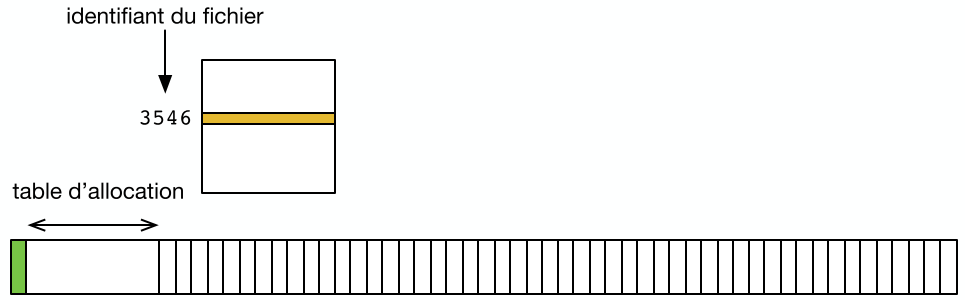
\includegraphics{image-40.png}
\caption{Alt text}
\end{figure}

Mais on doit s'intéresser à comment stocker un fichier et si sa taille
venait à changer.

\subsubsection{Option 1}\label{option-1}

On écrit simplement les blocs les un à la suite de l'autre et on stocke
simplement le pointeur vers l'entrée du premier blocs.

\begin{figure}
\centering
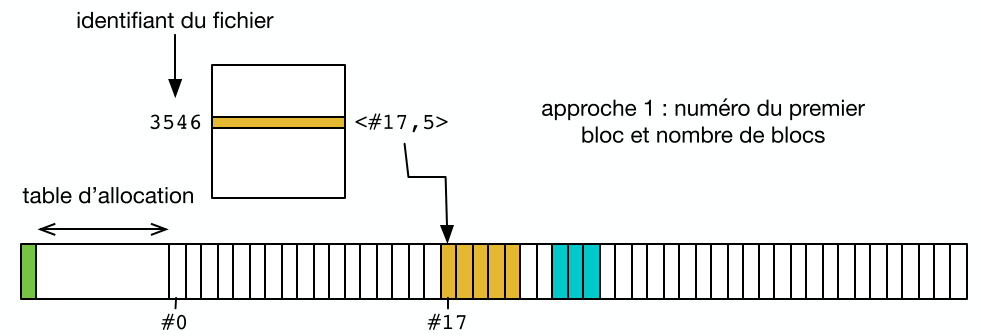
\includegraphics{image-41.png}
\caption{Alt text}
\end{figure}

\begin{itemize}
\tightlist
\item[$\boxtimes$]
  Simple
\item[$\square$]
  Compliqué d'agrandir un fichier
\item[$\square$]
  Fragmentation --\textgreater{} on a plein de blocs vides entre les
  blocs alloués
\end{itemize}

\subsubsection{Option 2}\label{option-2}

On stocke l'entrée pour le premier bloc puis on fait des pointeurs vers
le suivant etc etc ou avec un \texttt{EOF} (End Of File) si plus rien.

\begin{figure}
\centering
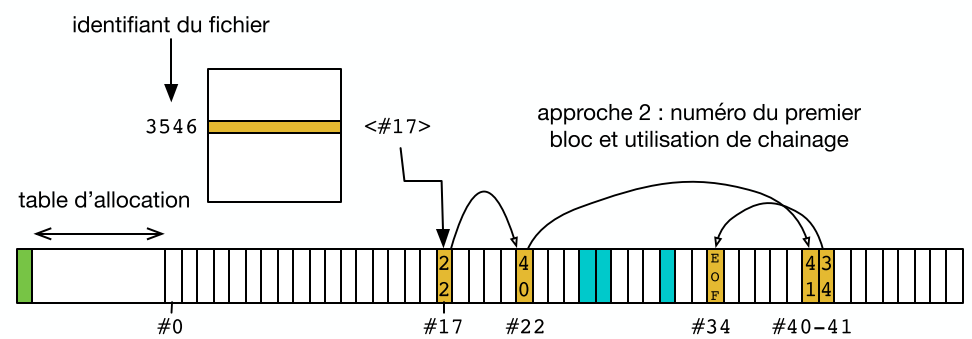
\includegraphics{image-42.png}
\caption{Alt text}
\end{figure}

\begin{itemize}
\tightlist
\item[$\boxtimes$]
  N'empêche pas de réserver tout l'espace libre
\item[$\square$]
  Localité HORRIBLE (le pire c'est sur un HDD)
\item[$\square$]
  On doit parcourir le fichier pour accéder au milieu
\end{itemize}

\subsubsection{FAT32}\label{fat32}

Pour \textbf{File Allocation Table} utilisé sur MS-DOS et Windows
(standard sur clé USB).

\paragraph{Combine 2 approches}\label{combine-2-approches}

On a une allocation des blocs \emph{contiguës} et liste chainé entre
\emph{groupe de blocs}. Croissance possible sans déplacement de blocs.

\begin{itemize}
\tightlist
\item[$\boxtimes$]
  Simple
\item[$\square$]
  Grande fragmentation et perte de la localité avec le temps
\end{itemize}

\paragraph{(Dé)Fragmentation}\label{duxe9fragmentation}

Une solution à ce problème est de \textbf{défragmenter} son disque.

Très important sur HDD, pas nécessaire sur Linux via \texttt{ext4} qui
prend des mesures en amont.

\subsubsection{Stockage indexé}\label{stockage-indexuxe9}

On ne va plus utiliser une table de en début de partition mais on va
utiliser certains blocs (\textbf{bloc d'index}) pour stocker les
métadonnées.

\begin{figure}
\centering
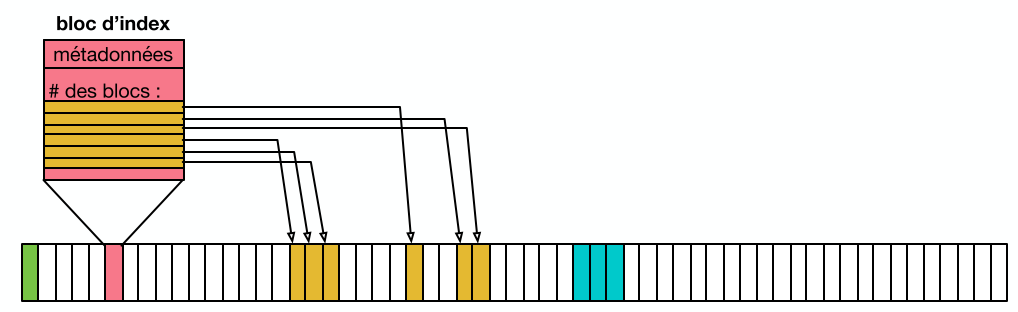
\includegraphics{image-43.png}
\caption{Alt text}
\end{figure}

\begin{itemize}
\tightlist
\item[$\boxtimes$]
  Pas de limitation à l'avance du nombre de fichiers.
\item[$\square$]
  On a besoin de 1 bloc en plus même pour des petits fichiers.
\end{itemize}

On peut utiliser tout l'espace mais on fait face à un risque
d'\emph{éparpillement}.

La taille du fichier est limité par la taille du bloc d'index.
--\textgreater{} si on a \texttt{4\ Ko} avec \texttt{4\ o} par entrée
cela signifie qu'on peut avoir que \texttt{800} entrées donc la taille
maximum est de \texttt{4\ Ko\ x\ 800} \textasciitilde{} \texttt{3\ Mo}.

\subsubsection{\texorpdfstring{Système de Fichiers
\texttt{ext4}}{Système de Fichiers ext4}}\label{systuxe8me-de-fichiers-ext4}

C'est le système de fichier standard et très généraliste et opti.

Mélange entre table d'allocation et blocs d'index. On a des
\emph{inodes} qui contient des métadonées et liens vers les blocs de
contenu.

Les inodes peuvent être inférieures à \texttt{4\ Ko}. Cela favorise la
localité des informations.

\begin{figure}
\centering
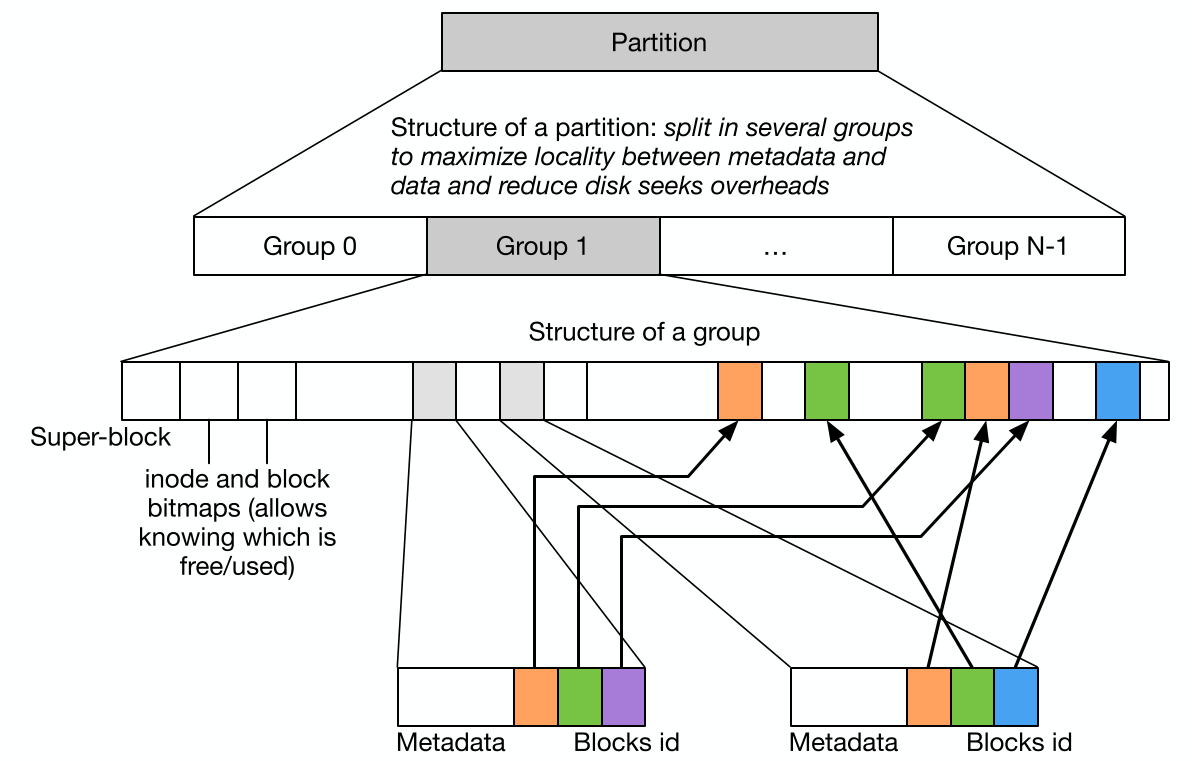
\includegraphics{image-44.png}
\caption{Alt text}
\end{figure}

L'idée c'est de faire des arbres d'inodes, donc on peut avoir des arbres
triples, doubles, simples , \ldots{}

\begin{figure}
\centering
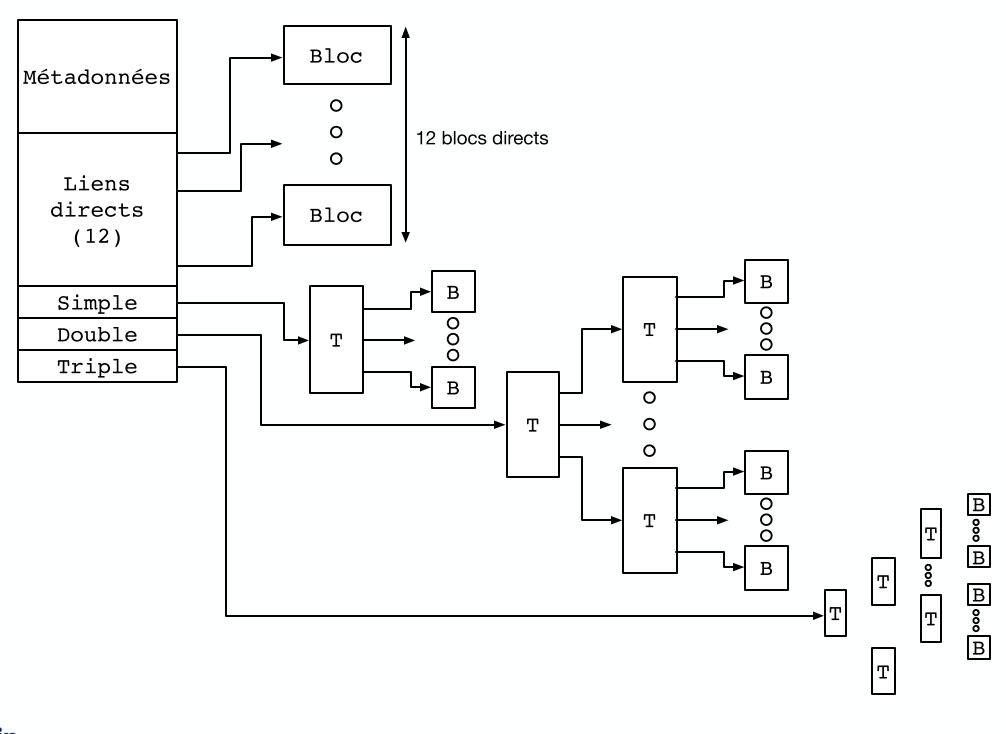
\includegraphics{image-45.png}
\caption{Alt text}
\end{figure}

\subsection{Stockage des Répertoires}\label{stockage-des-ruxe9pertoires}

Un répertoire est stocké comme un fichier. On va juste indiquer qu'il
s'agit d'un répertoire via des métadonnées via un bit \texttt{d}. On y
liste aussi les blocs de données (peut utiliser plusieurs blocs de
données).

Via \texttt{ext4}, stockage de petite liste de fichiers directement dans
l'inode.

\subsection{Gestion de l'Espace Libre}\label{gestion-de-lespace-libre}

On a une liste qui indique les blocs libres sur le disque qui est
conservé avec le temps.

\subsubsection{Effacer un Fichier}\label{effacer-un-fichier}

\texttt{rm} va juste supprimer l'entrée dans le répertoire et mettre
dans celle des blocs libres si plus aucun lien ne pointe vers ce
fichier.

L'inode et le bloc \textbf{ne sont pas effacés}. (donc on peut récupérer
des données même si elles ont été ``\emph{effacées}'')

\subsubsection{Performance et Cache}\label{performance-et-cache}

Un SSD est 1000 fois plus lent que de la RAM et un HDD est 1000000 de
fois plus lent. On va donc utiliser du cache.

\begin{figure}
\centering
\includegraphics{image-46.png}
\caption{Alt text}
\end{figure}

Le cache se situe au niveau du \textbf{contrôleur de périphérique et/ou
du disque}.

On peut utiliser la mémoire comme cache pour les accès disque. On peut
faire cela via la mémoire virtuelle et \texttt{mmap}.

\subsection{Optimisations}\label{optimisations}

\paragraph{Disque Dur}\label{disque-dur}

On va éviter de faire trop bouger la tête de lecture, donc on écrit sur
la partie la plus extérieure du disque.

On a un accès souvent séquentiel aux fichiers donc pas de retour en
arrière, on lit tout d'une traite: - \emph{read-ahead}: on charge les
blocs suivants - \emph{read-behind}: on libère les pages du cache au fur
et à mesure.

\begin{figure}
\centering
\includegraphics{Drawboard-PDF-Annotation-Copy.png}
\caption{Alt text}
\end{figure}

On va éviter les approches FIFO et privilégier soit une approche SSTF où
on se déplace du moins possible ou changer de direction le moins
possible via un algorithme de l'ascenseur.

\subsubsection{Robustesse}\label{robustesse}

Il faut que les données du disque restent cohérente malgré les mauvais
démontage, \ldots{}

On va donc avoir de la redondance et des vérificateurs de fichiers. On
peut vérifier que la liste des blocs vides ne pointent pas vers un bloc
listé par une inode.

\paragraph{Journalisation}\label{journalisation}

TODO

\begin{center}\rule{0.5\linewidth}{0.5pt}\end{center}

\href{../README.md}{\textless--}


\end{document}